\documentclass[a4paper, twoside, 11pt]{article}
% It is needed to use this command for automatic compilation in VSCode
% !TEX program = lualatexmk

%DOCUMENT, PREAMBLE AND MACROS DESIGNED FOR LuaLaTeX%
\newcommand{\fbar}{\FloatBarrier}
\usepackage{subfiles} % for subfiles
\usepackage{amsmath} %matematic package%
\usepackage{amssymb} %for miscellaneous mathematical symbols, first usage was for tick symbol in math mode \checkmark%
\usepackage{textcomp} %for miscellaneous symbols%
%\usepackage{times} %times font%
\usepackage{graphicx} %enhanced support for craphics%
%\usepackage{mathptmx} %use Times as default text font, and provide maths support%
\usepackage{cmap} %mapování znaků - vyhledávání v pdf%
\usepackage[english]{babel}%CZ%
\usepackage[utf8]{inputenc}%kódování%
\usepackage[T1]{fontenc}%kódování%
\usepackage{multirow}%Multirow table support
\usepackage{float}%Improves the interface for defining floating objects such as figures and tables%
\usepackage{wasysym} %for various glyphs, symbols%

\usepackage{setspace}%spacing% 
\onehalfspacing

\usepackage{hyperref}
\hypersetup{
    colorlinks=true, %pokud nechci definovat citecolor=black aby byly odkazy citací černé, tak dám colorlinks=false,%
    bookmarks=true,
    linkcolor=black,
    citecolor=black,
    urlcolor=black,
}

%when using LuaLaTex, defining Times Fonts from your system - it has to be named like this and inserted ttf file in the folder of your tex file%
\usepackage{fontspec}
\selectlanguage{czech}
\setmainfont[Ligatures=TeX,BoldFont={Times New Roman Bold}] {Times New Roman}
                                
\setsansfont[Ligatures=TeX,BoldFont={* Bold}]{Times New Roman}
                                      
\setmonofont{CourierPrime-Regular}
 
%\usepackage[italic]{mathastext} %for text in math environment, better looking times then



%for CITATIONS URL to work, it is not needed when you are not using URL label%
\usepackage{url}
\usepackage{csquotes}
\usepackage[style=iso-numeric, backend=biber, isbn=true, urldate=iso,seconds=true, date=terse, datezeros=true, language=czech]{biblatex}
\addbibresource{src/bib/zdroje.bib} % BIB resources to import
%\DeclareUrlCommand\url{\def\UrlLeft{<}\def\UrlRight{>} \urlstyle{tt}}



%\usepackage{biblatex}
%END for citations%

%changing bibliography font%
\renewcommand*{\bibfont}{\fontspec{Times New Roman}}

\usepackage{comment} %For comments%
\usepackage{pdfpages}%for pdf pages%
\usepackage{enumerate}%For lists%
\usepackage{enumitem}%For Custom Numbering Nested Lists%
\setlist[enumerate]{label*=\arabic*.} %setting Number. numbering in lists%
\usepackage{tikz} %For vector graphics%
\usepackage{circuitikz}%For schemes%
\usepackage{pgf} %Post script graphics for tikz%

%pouze funguje v PDFLaTeX%
%\usepackage{tgtermes}%na times font, jiný nefunguje s vyhledáváním a copy%

%
\usepackage{placeins}%% for \FloatBarrier command that blocks floating with htbp! go over \FloatBarrier
\usepackage{mathrsfs}%packagee for math symbols for Laplace, Z transform etc., usage \mathscr{Z}
\usepackage{upgreek}%for upgreek symbols, specified tau \uptau
\usepackage{physics}% for derivations \dd
%this works only when using PDFLaTeX%
\usepackage[list=true,listformat=simple]{subcaption}
\usepackage[figurename=Fig.,font=small,labelfont=it,textfont=it]{caption} %for renaming figures instead of renewcommand, small for 11pt default is 10pt as needed in word template
\usepackage[tablename=Tab.,font=small,labelfont=it,
            textfont=it]{caption} %for renaming tables instead of renewcommand

\usepackage{algorithm}
\usepackage{algpseudocode}
            
% List of abbreviations and symbols
% Original code author: Jakub Kučera

\usepackage[nonumberlist,nopostdot,section=subsection,numberedsection]{glossaries}
% section = subsection is for glossaries title to appear as a subsection, numberedsection adds the subsec number

\newglossary[slg]{symbolslist}{symbol}{ntn1}{List of symbols}
\newglossary[slg]{abbreviationslist}{abbreviation}{ntn2}{List of abbreviations}

\makeglossaries

% include files with definitions
% PZ definitions
\newglossaryentry{abbreviation:soc}{
                type=abbreviationslist,
                name={SoC},
                description={System on a chip}
}

\newglossaryentry{abbreviation:ip}{
                type=abbreviationslist,
                name={IP},
                description={Intellectual property}
}
\newglossaryentry{abbreviation:fpga}{
                type=abbreviationslist,
                name={FPGA},
                description={Field Programmable Gate Array}
}
\newglossaryentry{abbreviation:nr}{
                type=abbreviationslist,
                name={NR},
                description={Newton Raphson}
}
\newglossaryentry{abbreviation:rtl}{
                type=abbreviationslist,
                name={RTL},
                description={Register Transfer Level}
}
\newglossaryentry{abbreviation:fsm}{
                type=abbreviationslist,
                name={FSM},
                description={Finite State Machine}
}
\newglossaryentry{abbreviation:cordic}{
                type=abbreviationslist,
                name={CORDIC},
                description={Coordinate Rotation Digital Computer}
}
\newglossaryentry{abbreviation:lut}{
                type=abbreviationslist,
                name={LUT},
                description={Look Up Table}
}
\newglossaryentry{abbreviation:cpu}{
                type=abbreviationslist,
                name={CPU},
                description={Central Processing Unit}
}
\newglossaryentry{abbreviation:isa}{
                type=abbreviationslist,
                name={ISA},
                description={Instruction Set Architecture}
}
\newglossaryentry{abbreviation:foss}{
                type=abbreviationslist,
                name={FOSS},
                description={Free and Open-Source Software}
}
\newglossaryentry{abbreviation:she}{
                type=abbreviationslist,
                name={SHE},
                description={Selective Harmonic Elimination}
}
\newglossaryentry{abbreviation:vsi}{
                type=abbreviationslist,
                name={VSI},
                description={Voltage Source Inverter}
}
\newglossaryentry{abbreviation:dc}{
                type=abbreviationslist,
                name={DC},
                description={Direct Current}
}
\newglossaryentry{abbreviation:vcd}{
                type=abbreviationslist,
                name={VCD},
                description={Value Change Dump}
}

\newglossaryentry{symbol:Pn}{
    type=symbolslist, % glossary
    name=$P_\text{n}$, % jméno v seznamu
    description={jmenovitý výkon stroje}, %popis
    symbol = (W),
    sort=P % seředit podle
}



\newglossarystyle{myStyleAbbreviations}{
\renewenvironment{theglossary}%
     {\begin{longtable}[l]{llp{\glsdescwidth}p{\glspagelistwidth}}}%
     {\end{longtable}}%
  \renewcommand*{\glossaryheader}{}%
  \renewcommand*{\glsgroupheading}[1]{}%
  \renewcommand{\glossentry}[2]{%
  \glsentryitem{##1} \glstarget{##1}{##2} &
    \textbf{\glossentryname{##1}} &
    \glossentrydesc{##1} &
    ##2\tabularnewline
  }%
  \renewcommand*{\glsgroupskip}{}%  Pokud chci seskupovat podle abeced: \renewcommand*{\glsgroupskip}{ & \\}
}


\newglossarystyle{myStyleSymbols}{
  \renewenvironment{theglossary}%
    {\begin{longtable}[l]{llp{\glsdescwidth}p{\glspagelistwidth}}}%
    {\end{longtable}}%
  \renewcommand*{\glossaryheader}{}%
  \renewcommand*{\glsgroupheading}[1]{}%
  \renewcommand{\glossentry}[2]{%
    \glsentryitem{##1} \glstarget{##1}{\glossentryname{##1}} &
    \glossentrysymbol{##1} &
    \glossentrydesc{##1} &
    ##2\tabularnewline
  }%
  \renewcommand{\subglossentry}[3]{%
     &
     \glssubentryitem{##2}%
     \glossentrysymbol{##2} &
     \glstarget{##2}{\strut}\glossentrydesc{##2} & ##3\tabularnewline
  }%
  \renewcommand*{\glsgroupskip}{%
   }% Pokud chci seskupovat podel abecedy  \ifglsnogroupskip\else & & &\tabularnewline\fi
}
\renewcommand{\glossarypreamble}{\vspace*{-\baselineskip}} % deleting line after glossaries title

            %this works with LuaLaTex and fontspec package%
 \DeclareCaptionFont{times}{\fontspec{Times New Roman Italic}}

%labelfont and textfont defined here only works with previous declarecaptionfont times and fontspec%
\captionsetup{labelfont=times, textfont=times, labelsep=space}%no separator in captions
%

%\bibliographystyle{czechiso} %czechiso.bst in folder is needed for this style to work, available at http://www.fit.vutbr.cz/~martinek/latex/czechiso.html%

%\hyperref[label]{text}% Help for targeting labels

\usepackage{chngcntr} %for numbered figures with sections
\usepackage{tocloft}%better TOC

%\usepackage{a4wide}%širší a4%
\usepackage[inner=3cm,outer=2cm,top=2.5cm,bottom=2.5cm,footskip=1cm]{geometry}%for propper margins
\usepackage{textcase}%for making text uppercase without caps \MakeTextUppercase
 
 
\usepackage{titlesec}%for spacing text after sections
\usepackage{parskip}[]%for working \parskip
\newcommand{\sectionbreak}{\clearpage}%maybe for SECTIONS on a new page

\usepackage[titletoc]{appendix}%For appendix - přílohy, titletoc is crucial
%\renewcommand{\appendixname}{Příloha}

\setlength{\parindent}{0.5cm}%setting indent of paragraph to 0.5cm
\setlength{\parskip}{0em}%setting parskip to 0 for \titleformat to work properly with parskip package

\usepackage{colortbl}%for colored cells
\usepackage{xcolor}%for colors
\definecolor{ctublue}{HTML}{0065BD}%defining ctu color
\definecolor{ctugreen}{HTML}{A2AD00}
\definecolor{ctured}{HTML}{C60C30}
\definecolor{ctuyellow}{HTML}{F0AB00}
\definecolor{ctugreenyblue}{HTML}{00B2A9}
\definecolor{ctulightblue}{HTML}{6AADE4}
\definecolor{ctuorange}{HTML}{E05206}
\definecolor{lightgray}{HTML}{D1D5DB}
\definecolor{codeblue}{HTML}{D9E2F3}


\titlespacing*{\section}{0em}{1em}{-\parskip}%spacing text after sections from titlesec package
\titlespacing*{\subsection}{0em}{1em}{-\parskip}%spacing text after sections from titlesec package
\titlespacing*{\subsubsection}{0em}{1em}{-\parskip}%spacing text after sections from titlesec package

%when you want sectin/sub/subsub to be black, delete \color{ctublue}
\titleformat{\section}{\color{ctublue}\fontspec{Times New Roman}\fontsize{15}{15}\bfseries}{\thesection}{2.1em}{}%defining title sizes by word template
\titleformat{\subsection}{\color{ctublue}\fontspec{Times New Roman}\fontsize{14}{14}\bfseries}{\thesubsection}{1.53em}{}%defining title sizes by word template
\titleformat{\subsubsection}{\color{ctublue}\fontspec{Times New Roman}\fontsize{13}{13}\bfseries}{\thesubsubsection}{1em}{}%defining title sizes by word template


\usepackage{ctable}%imports xtable with booktabs
\usepackage{multicol}

\usepackage{listings}%for code environments - \begin{lstlisting}


\definecolor{codegreen}{rgb}{0,0.6,0}
\definecolor{codegray}{rgb}{0.5,0.5,0.5}
\definecolor{codepurple}{rgb}{0.58,0,0.82}
\definecolor{backcolour}{rgb}{0.95,0.95,0.92}


% solving problems with ) literal to be coded in lstlisting as it should be
\makeatletter
\patchcmd{\lsthk@SelectCharTable}{)}{`}{}{} 
\makeatother 

\lstdefinestyle{zakopal}{
    backgroundcolor=\color{codeblue},   
    commentstyle=\color{codegray},
    keywordstyle=\color{ctured},
    numberstyle=\tiny\color{codegray},
    stringstyle=\color{ctuorange},
    basicstyle=\ttfamily\small,
    breakatwhitespace=false,         
    breaklines=true,                 
    captionpos=b,                    
    keepspaces=true,                 
    numbers=left,                    
    numbersep=5pt,                  
    showspaces=false,                
    showstringspaces=false,
    showtabs=false,                  
    tabsize=2
}
\lstset{style=zakopal}
\renewcommand{\lstlistingname}{Code}% renaming Listing -> Kód 
\renewcommand{\lstlistlistingname}{List of codes}% renaming List of Listings -> Seznam kódů

\lstdefinelanguage{SCL}
{morekeywords={FUNCTION_BLOCK,BEGIN,NOT,END_FUNCTION_BLOCK,FUNCTION,VOID,VAR_INPUT,END_VAR,VAR_IN_OUT,IF,
THEN,END_IF,END_FUNCTION,BOOL,FALSE,TRUE},
sensitive=false,
morecomment=[l]{//},
morestring=[b]",
literate={;}{{\textcolor{ctuorange}{;}}}{1}
{:}{{\textcolor{ctuorange}{:}}}{1}
{)}{{\textcolor{ctuorange}{)}}}{1}
{(}{{\textcolor{ctuorange}{(}}}{1}
{=}{{\textcolor{ctuorange}{=}}}{1}
{,}{{\textcolor{ctuorange}{,}}}{1},} %basic SCL language for siemens defined%

\lstdefinelanguage{xdc}
{morekeywords={set_property, current_design, get_ports},
sensitive=false,
morecomment=[l]{\#}} %basic xdc file in Vivado syntax highlighting%

\lstdefinelanguage{xsct}
{morekeywords={xsct, hsi, open_hw_design, -createdts, -hw, -zocl, -platform-name, -overlay, -compile, -out, exit, -git-branch},
alsoletter={-},
sensitive=false,
morecomment=[l]{\#}} %xsct (Xilinx Software Command-Line Tools)%


\lstdefinelanguage{Text}
{morekeywords={},
alsoletter={-},
sensitive=false,
morecomment=[l]{//},
morecomment=[l]{\#}} %basic text%

\lstdefinelanguage{devicetree}
{morekeywords={chosen, bootargs, stdout-path, compatible, status},
alsoletter={-},
stringstyle=\color{ctuorange},
moredelim=[s][\color{ctuorange}]{"}{"},
sensitive=false,
morecomment=[l]{\#},
literate={\{}{{\textcolor{ctured}{\{}}}{1}
{\}}{{\textcolor{ctured}{\}}}}{1}
} %devicetree%

\lstdefinelanguage{json}
{morekeywords={},
upquote=true,
morestring=[b]",
stringstyle=\color{ctuorange},
moredelim=[s][\color{ctuorange}]{"}{"},
sensitive=false,
morecomment=[l]{\#},
literate=
     *{0}{{{\color{ctured}0}}}{1}
      {1}{{{\color{ctured}1}}}{1}
      {2}{{{\color{ctured}2}}}{1}
      {3}{{{\color{ctured}3}}}{1}
      {4}{{{\color{ctured}4}}}{1}
      {5}{{{\color{ctured}5}}}{1}
      {6}{{{\color{ctured}6}}}{1}
      {7}{{{\color{ctured}7}}}{1}
      {8}{{{\color{ctured}8}}}{1}
      {9}{{{\color{ctured}9}}}{1}
      {\{}{{{\color{ctured}{\{}}}}{1}
      {\}}{{{\color{ctured}{\}}}}}{1}
      {[}{{{\color{ctured}{[}}}}{1}
      {]}{{{\color{ctured}{]}}}}{1},
} %json%

\lstdefinelanguage{pseudocode}
{morekeywords={if, else, positive, negative, edge, end},
alsoletter={-},
stringstyle=\color{ctuorange},
moredelim=[s][\color{ctuorange}]{"}{"},
sensitive=false,
morecomment=[l]{\//},
literate={\{}{{\textcolor{ctured}{\{}}}{1}
{\}}{{\textcolor{ctured}{\}}}}{1}
{(}{{{\color{ctured}{(}}}}{1}
{)}{{{\color{ctured}{)}}}}{1}
{\&}{{{\color{ctublue}{\&}}}}{1}
{=}{{{\color{ctublue}{=}}}}{1}
{<}{{{\color{ctublue}{<}}}}{1}
{>}{{{\color{ctublue}{>}}}}{1}
} 
%%change in previous commands 2.1 em , 1.53em and 1em to 1em to be easy indented not the same
\begin{document}
\fontspec{Times New Roman}

\counterwithin{figure}{section}%changing counter of figure, at each section the numbering resets
\counterwithin{table}{section}%changing counter of table, at each section the numbering resets
\counterwithin{equation}{section}%changing counter of equation, at each section the numbering resets

\counterwithin{lstlisting}{section}%counter of lstlist - codes, reseting at each section%


\renewcommand{\thefigure}{\thesection~-~\arabic{figure}}%defining style of countering
\renewcommand{\thetable}{\thesection~-~\arabic{table}}
\renewcommand{\theequation}{\thesection~-~\arabic{equation}}
\renewcommand{\thelstlisting}{\thesection~-~\arabic{lstlisting}}%delfining style for lstlisting codes, needs to be after begin document as previous renewcommand%

\renewcommand*{\cftsecdotsep}{1}  % use dots in the section entries and their step
\renewcommand*{\cftsubsecdotsep}{1}
\renewcommand*{\cftsubsubsecdotsep}{1}
\renewcommand*{\cftsecnumwidth}{4em} % increase space for Roman numerals
\renewcommand*{\cftsubsecnumwidth}{4em} %numbering width
\renewcommand*{\cftsubsubsecnumwidth}{4em} %numbering width
\renewcommand*{\cftsubsubsecindent}{0em}%no indent for subsubsection
\renewcommand*{\cftsubsecindent}{0em}%no indent for subsection
\renewcommand*{\cftsecindent}{0em}%no indent for subsection



\renewcommand*{\cftfigdotsep}{1}  % use dots in the figure entries and their step
\renewcommand*{\cftfignumwidth}{4em}
\renewcommand*{\cftfigindent}{0em}

\renewcommand*{\cfttabdotsep}{1}  % use dots in the figure entries and their step
\renewcommand*{\cfttabnumwidth}{4em}
\renewcommand*{\cfttabindent}{0em}

\renewcommand{\cftsecfont}{\fontspec{Times New Roman}\large \bfseries}
\renewcommand{\cftsubsecfont}{\fontspec{Times New Roman}}
\renewcommand{\cftsubsubsecfont}{\fontspec{Times New Roman}}

\renewcommand{\cftfigfont}{\fontspec{Times New Roman}}
\renewcommand{\cfttabfont}{\fontspec{Times New Roman}}

\renewcommand*\contentsname{\textcolor{ctublue}{\MakeTextUppercase{\fontspec{Times New Roman}Table of Contents}}}
\renewcommand{\listtablename}{{\fontspec{Times New Roman}\textcolor{ctublue}{\MakeTextUppercase{{List of tables}}}}}
\renewcommand{\listfigurename}{{\fontspec{Times New Roman}\textcolor{ctublue}{\MakeTextUppercase{{List of figures}}}}}



%\renewcommand{\thefigure}{\arabic{section}.\arabic{figure}}%changing figure name to be section.subsection. but do no reset
\setcounter{figure}{0}

\begin{titlepage}
	\begin{center}

\begin{figure}[H]
	\begin{center}
		
\includegraphics[scale=1]{src/misc/symbol_cvut_konturova_verze.pdf}
	\end{center}
\end{figure}
	{\Large{\textbf{CZECH TECHNICAL UNIVERSITY IN PRAGUE}}}\\
	{\textbf{Faculty of Electrical Engineering}}\\
	{\textbf{Department of Electric Drives and Traction}}
	
	\vspace{3cm}
	
	
	{\Large\textbf{Low Abstraction Real-Time FPGA Implementation of Selective Harmonic Elimination Algorithm for Voltage Source Inverters Designed Using State of The Art Free and Open Source Software}}
	
	\vspace{1cm}
	
	%{\Large\textbf{Possibilities of Using SoC Platform Processors for Controlling Electric Drives}}
	
	%\vspace{2cm}
	
	Technical report\\
	
	\end{center}
	
	\vspace{3cm}
	
	%\noindent Studijní program: Elektrotechnika, Energetika a Management\\
	%\noindent Studijní obor: Elektrické pohony
	
	\vspace{0.5cm}
	%\noindent Vedoucí práce: doc. Ing. Jan Bauer, Ph.D.
	
	\vfill
	
\begin{center}

	\large{\textbf{Petr Zakopal}}\\
	\large{\textbf{Prague 2023}}
	\end{center}
\end{titlepage}


\newpage
%\pagenumbering{arabic} to arabic page numbering
\pagenumbering{gobble} %disabling page numbering

\newpage


%%ZADÁNÍ PRÁCE
%verze pro TISK - jen s NEW PAGE


%ONLINE VERZE - se zadáním BEZ PODPISŮ
% online verze - odkomentovat následující dva řádky
%\null\newpage
%\includepdf[]{src/docs/zadani_bez_podpisu.pdf}

%\newpage
%\cleardoublepage
\null\newpage

\pagenumbering{Roman}
\setcounter{page}{2}%%3 NUTNO řešit dle zadání etc.

% \noindent \textcolor{ctublue}{{\Large{\textbf{\MakeTextUppercase{Prohlášení}}}}}\\
% 			Prohlašuji, že jsem předloženou práci vypracoval samostatně a že jsem uvedl veškeré použité informační zdroje v~souladu s~Metodickým pokynem o~dodržování etických principů při přípravě vysokoškolských závěrečných prací.\\
% 		\vspace{1.5cm}
		
	

% 	\noindent	V~Praze dne \rule{3.5cm}{0.4pt} \hspace{6.6cm}  \rule{4cm}{0.4pt}
	
% 	\hspace{12.65cm}Petr Zakopal


% 		\vspace{14cm}
		
% 	\noindent	\textcolor{ctublue}{{\Large{\textbf{\MakeTextUppercase{Poděkování}}}}}\\
% 	Tímto bych rád poděkoval vedoucímu této práce doc. Ing. Janu Bauerovi, Ph.D. za skvělé vedení práce a cenné rady při jejím vytváření. Dále bych rád poděkoval všem, kteří mě v~mém dosavadním studiu podporovali.
		


%%ABSTRAKT%%

% \newpage
% %\addcontentsline{toc}{section}{3\quad Abstrakt a klíčová slova}%Added citations to TOC%
% %\begin{comment}
% \begin{minipage}[t]{7.37cm}
% 		%\raggedright
% 	\textcolor{ctublue}{\Large{\textbf{\MakeTextUppercase{Abstrakt}}}}\\
	
% \end{minipage}%
% \hfill% --- important, otherwise it wont be so nice
% \begin{minipage}[t]{7.37cm}
% 		\textcolor{ctublue}{\Large{\textbf{\MakeTextUppercase{Abstract}}}}\\
		
% \end{minipage}
% %\end{comment}
% 	%\textcolor{ctublue}{\Large{\textbf{\MakeTextUppercase{Abstrakt}}}}\\

% 	%\textcolor{ctublue}{\Large{\textbf{\MakeTextUppercase{Abstract}}}}\\

% \newpage
\tableofcontents
\newpage%
\flushbottom %vyčištění stránky
\newpage
\vspace{0pt}
\listoffigures %seznam obrázků
\flushbottom %vyčištění stránky
\newpage
\listoftables
\flushbottom
\newpage


\pagenumbering{arabic} %to arabic page numbering - enabling page numbering after gobble which disabled page numbering
\pagenumbering{gobble}
\null\newpage
% \null\newpage %PŘI VERZI ONLINE
\setcounter{page}{1}
\pagenumbering{arabic}
\fontspec{Times New Roman}

\section{Introduction}
This paper presents the design of multiple \gls{abbreviation:fpga} units, which are designed to suit near real-time constraints of controlling the electric drives or for Hardware In Loop systems.\par
The goal of this paper also was to investigate how to design the speed optimized units using open source toolchain. The final designed unit is capable of solving the Selective Harmonic Elimination (\gls{abbreviation:she}) algorithm. Many researches opt for proprietary design software, which very often offers premade Intelectual Property (\gls{abbreviation:ip}) blocks, which can be used to design the specified circuit. However in this paper the design was created, tested and analyzed solely using the State of The Art Open Source software without any \gls{abbreviation:ip} catalogs. This platformless solution ensures, that the designed units may possibly be synthetized for various \gls{abbreviation:fpga} chips without any major barriers.\par
The structure of the paper is as follows: Section \ref{sec:calculating-the-division-of-fixed-point-numbers} presents a unit for division of two arbitrary values by utilizing the Newton-Raphson (\gls{abbreviation:nr}) algorithm. Section \ref{sec:using-cordic-to-calculate-trigonometric-functions} presents design of the Coordinate Rotation Digital Computer (\gls{abbreviation:she}) optimized for speed, rather than lesser complexity. Section \ref{sec:simple-set-of-nonlinear-equations-solved-by-a-newton-raphson-algorithm-using-custom-circuit-implementation} introduces design which solves two non-linear equations with a Newton-Raphson (\gls{abbreviation:nr}) algorithm, presenting suitability of \gls{abbreviation:fpga} designs for iterative algorithms. Section \ref{sec:selective-harmonic-elimination} presents unit for solving the Selective Harmonic Elimination problem using previously developed modules.

\flushbottom %vyčištění stránky
\newpage
%konec úvodu

\section{Notes on all of the circuit designs in Verilog}
    All of the designs presented in this paper are created using pure Verilog code and tested through Free and Open-Source Software (\gls{abbreviation:foss}). The decision to opt for \gls{abbreviation:foss}  was deliberate, aiming to prevent any vendor-locking to specific hardware or predefined \gls{abbreviation:ip}s. Predefined \gls{abbreviation:ip}s  are often optimized by a specific hardware vendor and intended for use with that vendor's hardware. However, the hardware may not always be available or suitable for a specific application. Academics and numerous companies opt for open-source and open-hardware approaches to prevent vendor lock-in. Once the design and algorithm are thoroughly understood, they can be initially implemented without any specific platform in mind. Later, when selecting the device vendor, the design can be modified to suit the specific hardware requirements.\par
    That is why Verilog, with Cocotb \cite{cocotb} (Test Bench creation tool) and Verilator \cite{verilator} (simulator) have been used for designing the circuits presented in this paper.\par

\section{Calculating the division of fixed point numbers}\label{sec:calculating-the-division-of-fixed-point-numbers}
Typically, when employing numerical methods to solve transcendental equations, the calculation of the division of two input numbers becomes necessary. This requirement persists even when applying the Newton-Raphson (\gls{abbreviation:nr}) method to solve a set of two equations, because computing the reciprocal value of the Jacobian determinant.\par
There are some \gls{abbreviation:ip} blocks available, which are capable of calculating the division of two numbers, but the blocks are usually either vendor specific intellectual property \gls{abbreviation:ip} \cite{amd-xilinx-vivado-divider-ip-block} or feature low performance \cite{burke-fixed-point-math-library}.\par
The drawback of vendor-specific \gls{abbreviation:ip}s lies in their limited compatibility, often preventing their use with \gls{abbreviation:fpga} chips from different vendors. On the other hand the vendor specific \gls{abbreviation:ip}s are usually optimized and able to use the specific type of resources available at the vendor's chip which resolve in better performance.\par
To preserve the compatibility of the design with chips from multiple vendors, the custom solution for division design based on the very known Newton Raphson (\gls{abbreviation:nr}) algorithm was developed. \cite{burke-fixed-point-math-library}

\subsection{Newton Rapshon algorithm for calculating the division}\label{subsection:newton-raphson-algorithm-for-calculating-the-division}
General Newton Raphson (\gls{abbreviation:nr}) algorithm is a well known approach to numerically solve equations. It is the reason why it is utilized in many algorithms. However, the negative aspect of \gls{abbreviation:nr} is that it's convergency strongly depends on initial values of variables. When the initial values are chosen poorly, the performed number of iterations before the convergency is reached can be high.\par
To reach the fastest convergency possible (determined in number of iterations) apart from the scaling the dominator into the interval [0.5,1] the initial value calculation formula should be utilized. \cite{burke-fixed-point-math-library}\par
The Equation \ref{eq:initial-nr-value-formula} for calculating the initial value  is applied after the scaling of denominator is performed. The algorithm developed for the appropriate scaling is explained in the \hyperref[subsec:calculating-number-of-bits-to-shift-the-denominator]{\textit{Calculating number of bits to shift the denominator}}.

\begin{equation}\label{eq:initial-nr-value-formula}
x_0 = \frac{48}{17} - \frac{32}{17} D,
\end{equation}
where the $x_0$ is the initial value for \gls{abbreviation:nr} algorithm, $D$ is the denominator value for calculating the expression $N/D$.\par
Because in the module design implemented via Verilog the fixed point number format \textit{Q32.15} is used, the fractional numbers from Equation \ref{eq:initial-nr-value-formula} are rounded to\newline2.8229 (32'sb00000000000000010\_110100101011000 in binary)\newline and 1.8819 (32'sb00000000000000001\_111000011100101 in binary) respectively.\par
After the initial value $x_0$ is calculated, the \gls{abbreviation:nr} algorithm is performed. The idea of using \gls{abbreviation:nr} algorithm to calculate the division of $N/D$ is to trade the division for a multiplication which can be synthetized in the \gls{abbreviation:fpga} fabric. When employing the \gls{abbreviation:nr} algorithm for finding the values of $N/D$ the function with root is $1/D$ is essential. After the root of the function is found, it is then multiplied by the numerator value, and te solution $N/D$ is obtained. There may be many functions, which root is the searched value $1/D$ but the most trivial is Equation \ref{eq:equation-with-appropriate-root}.\par

\begin{equation}\label{eq:equation-with-appropriate-root}
  \text{F} (x_i) = \frac{1}{x_i} - D.
\end{equation}

\noindent For the derivative at the point of $x_i$ then applies Equation \ref{eq:nr-division-derivative-at-the-point}.

\begin{equation}\label{eq:nr-division-derivative-at-the-point}
  \frac{\dd F(x_i)}{\dd x} = F'(x_i) = \frac{F (x_{i+1}) - F (x_i)}{x_{i+1}-x_i}.
\end{equation}

\noindent Because finding root of the equation \ref{eq:equation-with-appropriate-root}, the value of $F (x_{i+1})$ is set to be zero. After separating the $x_{i+1}$ value of the eq. \ref{eq:nr-division-derivative-at-the-point} and derivating the function $F (x_i)$ the obtained algorithm for a value $x_{i+1}$ is obtained from eq. \ref{eq:derivative-nr-new-value-algorithm}.\par

\begin{equation}\label{eq:derivative-nr-new-value-algorithm}
  x_{i+1} = -\frac{F (x_i)}{F' (x_i)} + x_i = - \frac{F (x_i)}{-\frac{1}{x_i^2}} + x_i = (\frac{1}{x_i} - D) x_i^2 + x_i = x_i - D x_i^2 + x_i = 2 x_i - D x_i^2.
\end{equation}

Usually, the iterative algorithm is stopped, when the value $F(x_{i+1}) - F(x_i)$ (called defect) reaches certain value set by the stop condition. However, in this algorithm, the stop condition is not yet implemented. Based on the observation carried on the N-R algorithm the obtained result is sufficient after 5 iterations.

The mathematically expressed algorithm is then transformed into programmable algorithm suitable for \gls{abbreviation:fpga} implementation. The top module design for this algorithm is presented in the section \hyperref[subsubsec:division-top-module-design]{\textit{Top module design}}, the control and data unit for calculating the value $x_{i+1}$ is presented in the \hyperref[subsubsec:division-allocation-and-timing]{\textit{Allocation and Timing}}

\subsection{IP Block Design}\label{subsec:division-ip-block-design}
The design of this unit is consists of 4 main modules:
\begin{itemize}
  \item the \textbf{data unit module}, used for manipulating data and making calculation operations,
  \item the \textbf{control unit module}, used for controlling the \textbf{data unit module} and \textbf{scaling unit module},
  \item \textbf{scaling unit module}, used for calculating the number of bits needed for shifting the denominator value to the interval [0.5,1].
\end{itemize}
\subsubsection{Top module design}\label{subsubsec:division-top-module-design}
The top module wraps all of the presented modules (\textbf{data unit module}, \textbf{control unit module}, \textbf{scaling unit module}). The basic structure of connected modules of this top design is depicted in the Figure \ref{fig:division-top-module}. Thanks to this wrapper it is possible to test the created modules with Verilog Testbench, Verilator \cite{verilator} or Cocotb \cite{cocotb}.
\begin{figure}[htbp!]
  \centering
  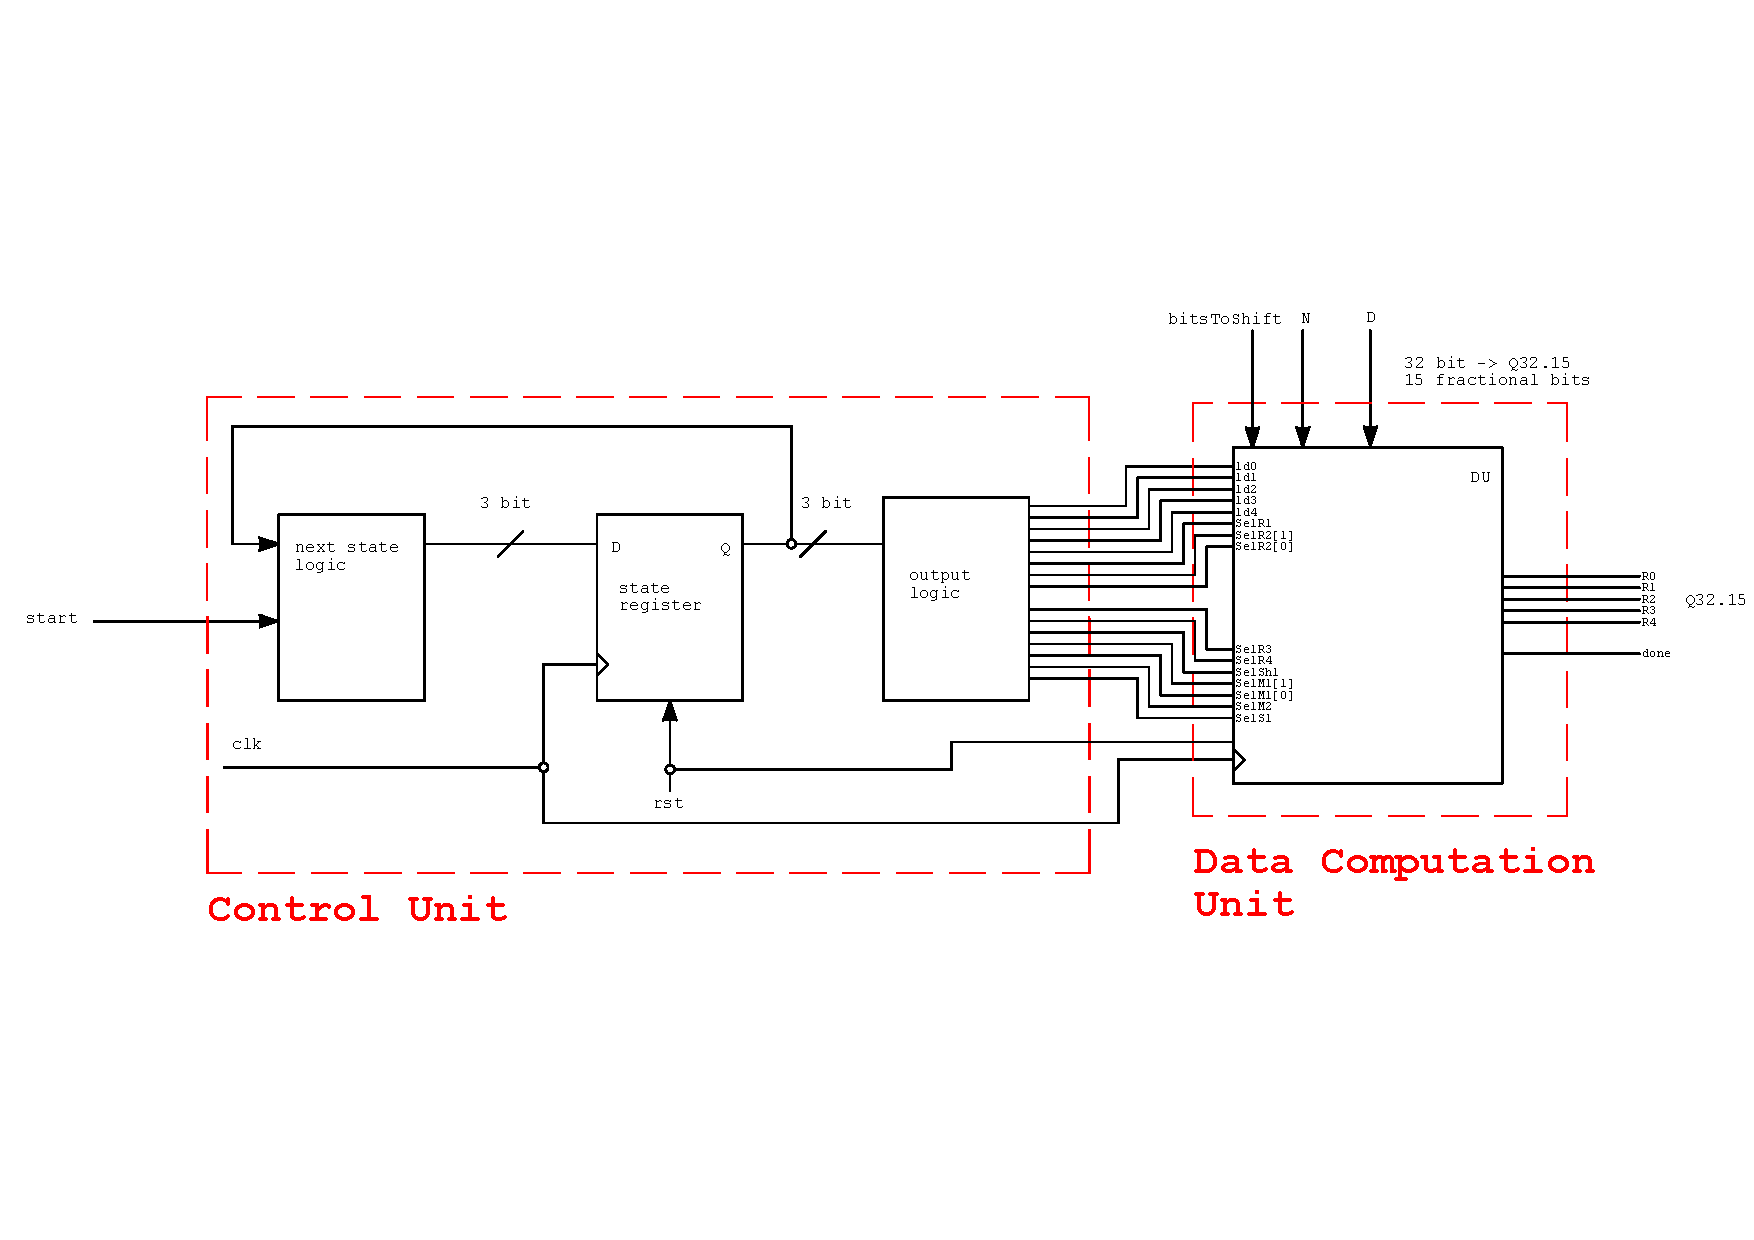
\includegraphics[width=1\textwidth]{src/pdf/top-module.pdf}
   \caption{Top module design for the division unit module block design.}
  \label{fig:division-top-module}
\end{figure}



\fbar
\subsubsection{Allocation and Timing}\label{subsubsec:division-allocation-and-timing}
The diagram of the data flow and timing of the algorithm is displayed in the Figure \ref{fig:division-allocation-timing}.\par
The whole algorithm comprises nine steps. The initial four steps are used for calculating the initial value of $x_0$ as presented in the Equation \ref{eq:initial-nr-value-formula}. The steps \textit{S4} to \textit{S8} are for calculating the next search value of $x_{i+1}$, thus the root of the Equation \ref{eq:equation-with-appropriate-root} which in fact is the searched value of $1/D$. The following iteration begins at the step labeled as \textit{S5}. The iterative process continues until a predefined stop condition is satisfied, such as reaching a specified number of iterations.
\begin{figure}[htbp!]
  \centering
  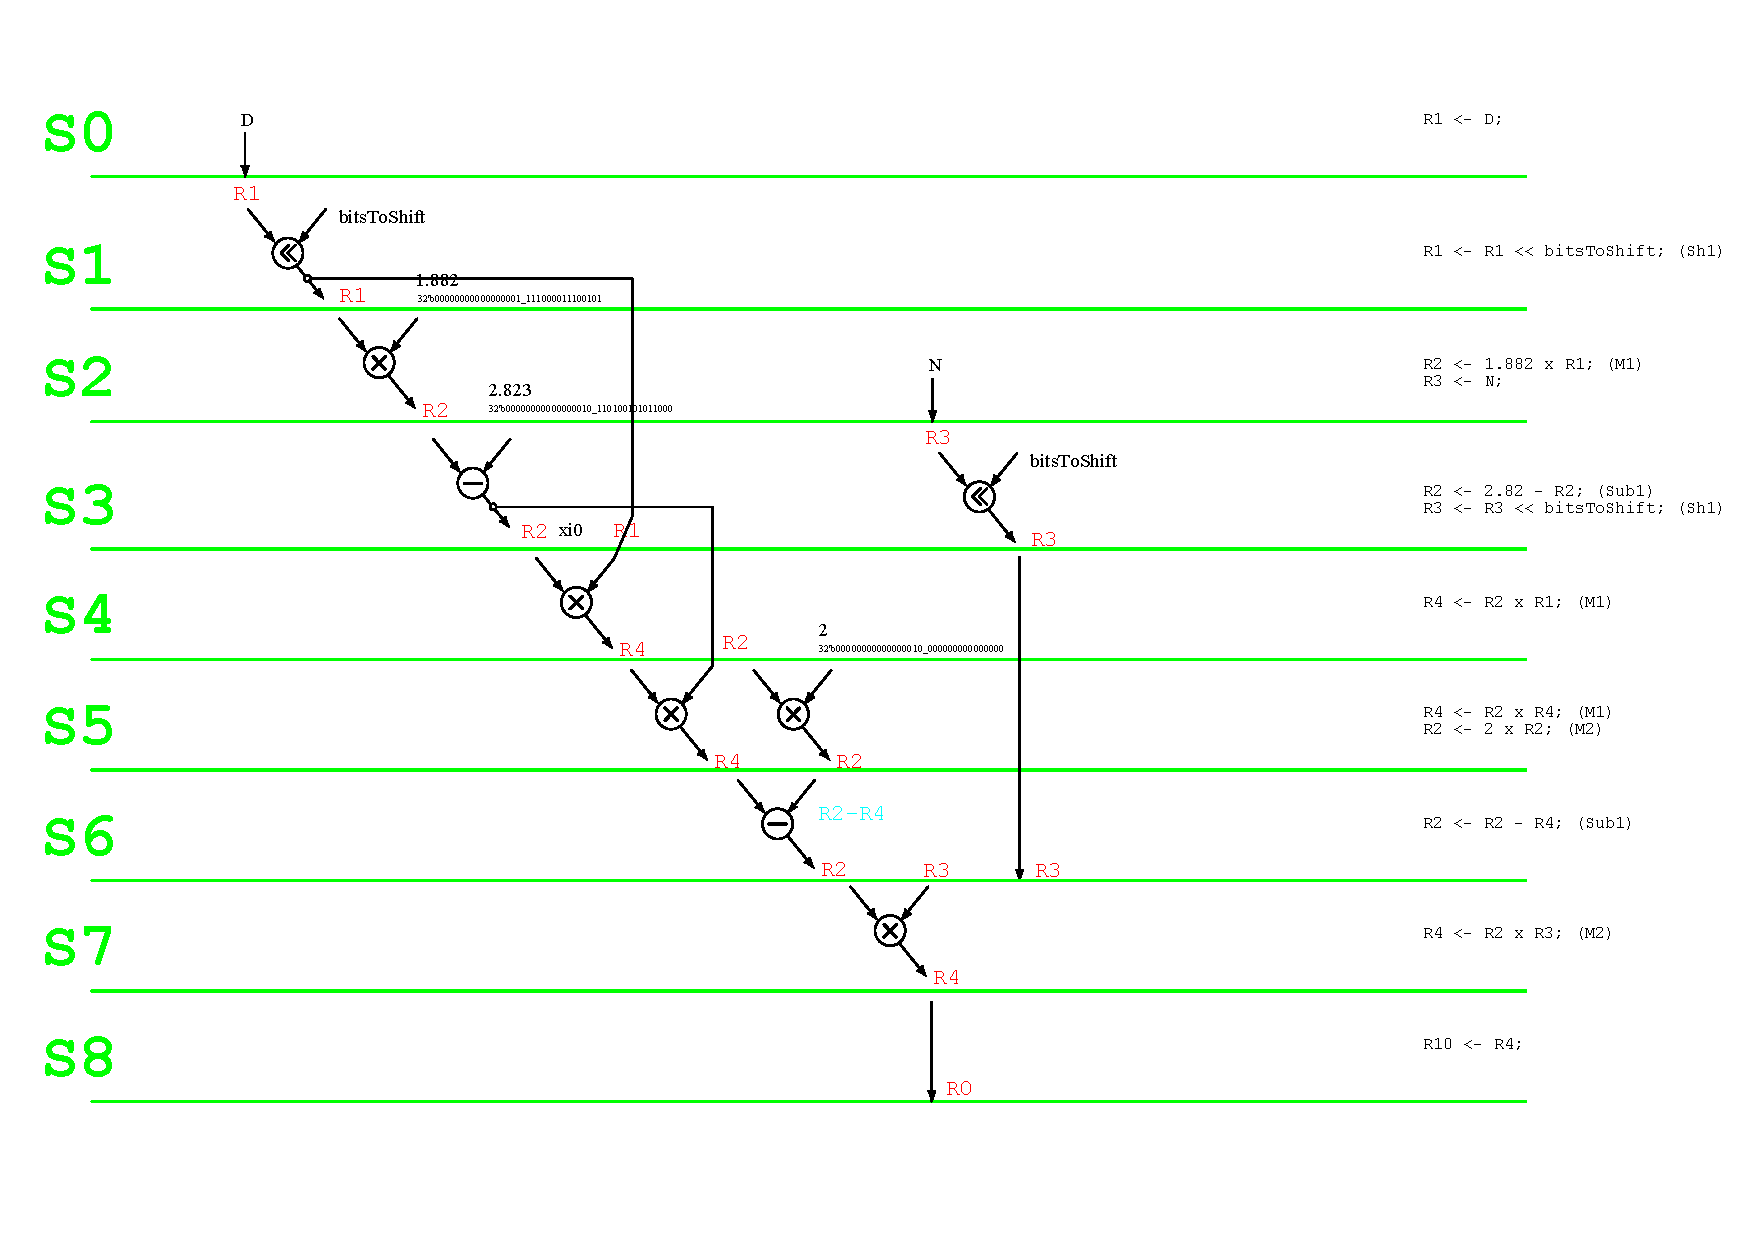
\includegraphics[width=1\textwidth]{src/pdf/allocation-timing.pdf}
   \caption{Alloccation and timing diagram for the Data Path Unit part of the division module.}
  \label{fig:division-allocation-timing}
\end{figure}

\fbar
\subsubsection{Data Path Module}
The structure of the Data Path Module is depicted in the Figure \ref{fig:division-rtl}. The module was specifically designed to serve the needs of the division algorithm. It comprises five registers labeled $R0$ through $R4$, two multipliers $M1$, $M2$ and one bit shifter.\par
The module is controlled by the control unit using the control signal labeled as CS. The encoding table with the labels corresponding to the Data Path Unit module is presented in the section \hyperref[subsubsec:division-control-unit]{\textit{Control Unit}}.\par
The result of each iteration from the division algorithm is passed to a register $R0$.\par
The Data Path Module unit also covers the possibility of using negative denominator and numerator. Because the values are stored in a custom \textit{Q32.15} fixed point format (whole number comprises of 32 bits, 15 bits fractional part, 17 bits integer part), the algorithm checks if the $D$ or $N$ values are higher than $0h8000$ and determine it's actual sign and the sets sign of the result. If the analyzed number is determined negative, it is transformed to value positive and then used in the presented division algorithm. This transformation is needed because of the algorithm calculating the bits to shift the denominator in the interval.
\begin{figure}[htbp!]
  \centering
  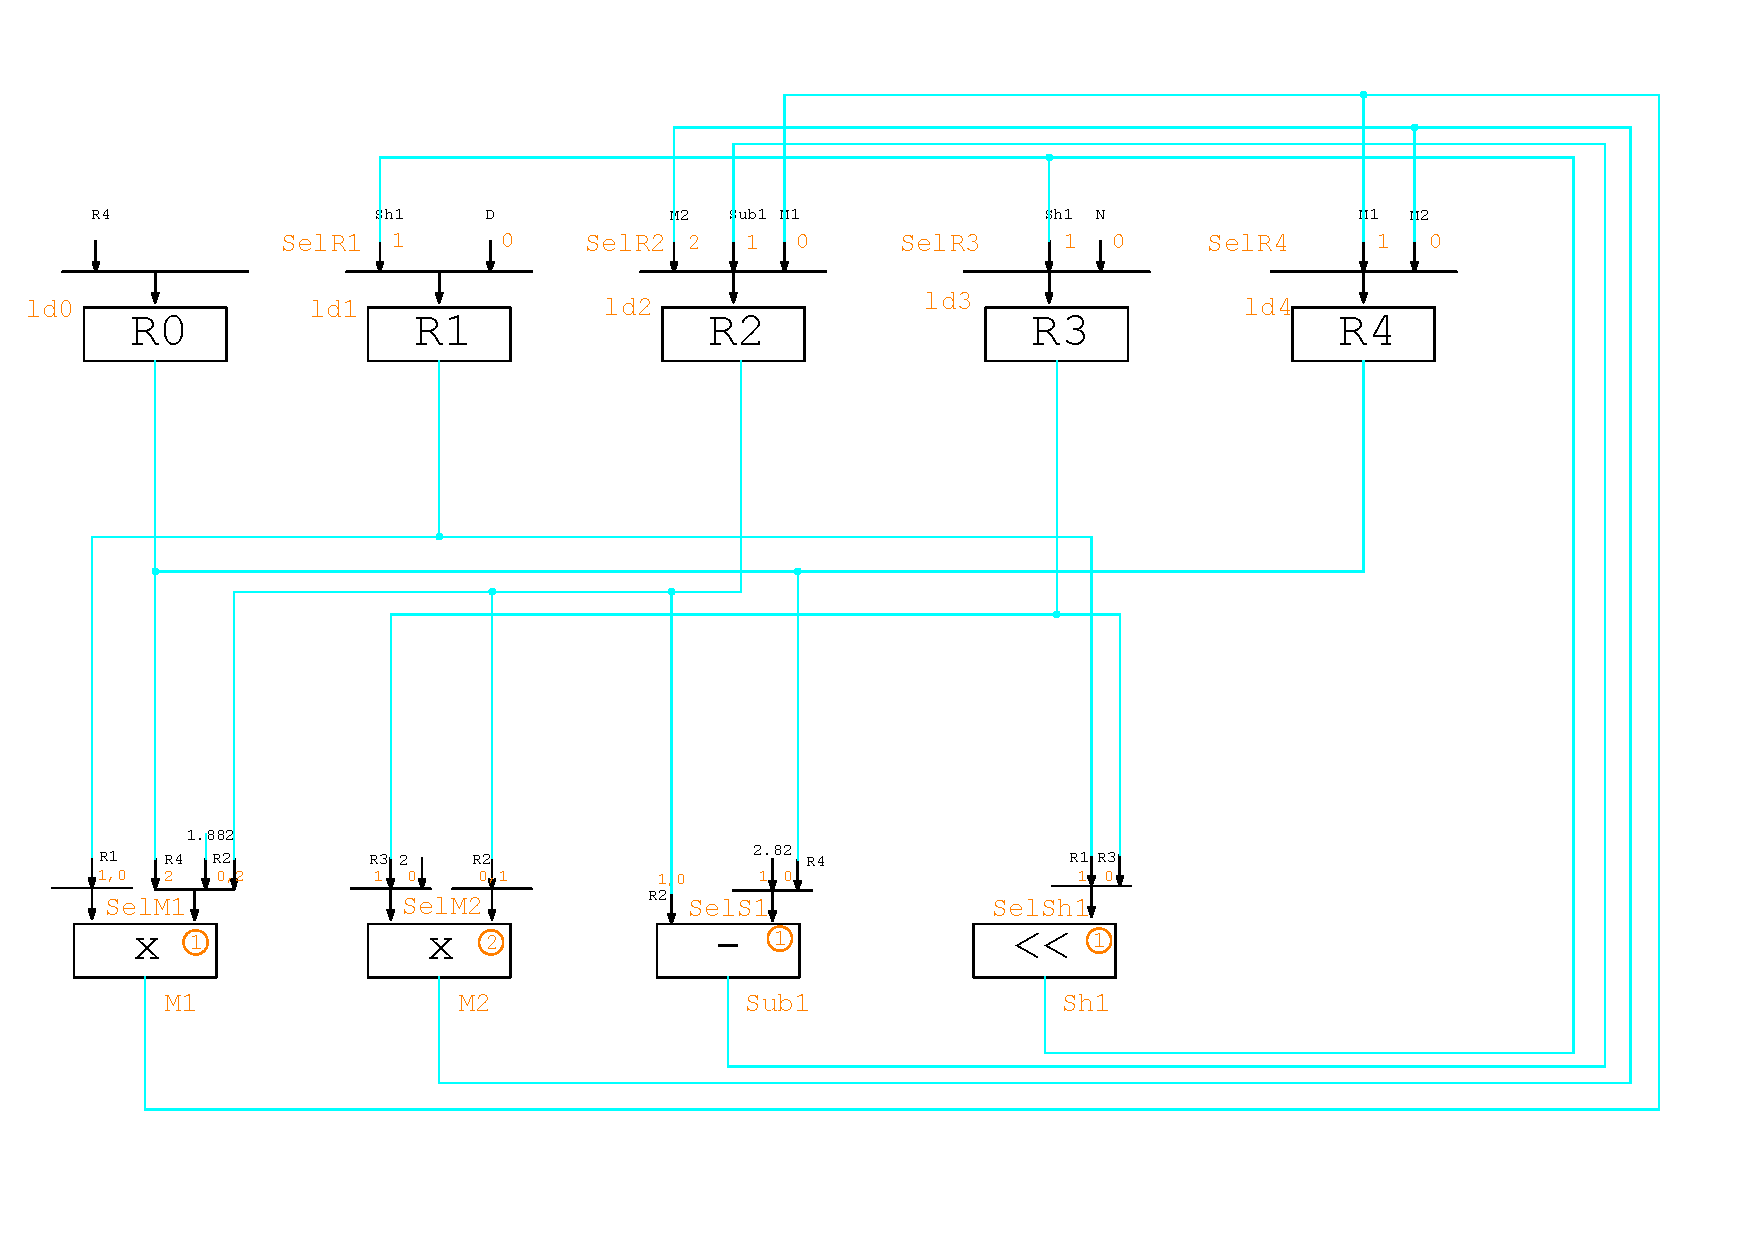
\includegraphics[width=1\textwidth]{src/pdf/rtl.pdf}
    \caption{Register Transfer Level (\gls{abbreviation:rtl}) scheme of the Data Path Unit part of the division module.}
  \label{fig:division-rtl}
\end{figure}


\fbar
\subsubsection{Control Unit}\label{subsubsec:division-control-unit}
Signals from Control Unit to Data Path Module are encoded in the CS signal. Table \ref{tab:control-signal-division-unit} displays the CS signal along with the corresponding instructions for steps $S0$–$S8$ of the \gls{abbreviation:fsm}. To enhance code clarity the signal is passed to the Control Unit in the hexadecimal format.\par
The number of the iteration of the Finite State Machine (\gls{abbreviation:fsm}) is also set in the Control Unit. This iteration number is subsequently used in the module to check for the stop condition of the calculation loop.\par
As stated in the \hyperref[subsubsec:division-allocation-and-timing]{\textit{Allocation and Timing}} section, after the step \textit{S8}, the \gls{abbreviation:fsm} restarts at the state \textit{S4} with new $x_i$ values as inputs. This state change is not depicted in the Table \ref{tab:control-signal-division-unit} for CS signal.

\subfile{src/tex/division-control-unit-table.tex}
\fbar

\subsection{Calculating number of bits to shift the denominator}\label{subsec:calculating-number-of-bits-to-shift-the-denominator}
As presented in the section \hyperref[subsection:newton-raphson-algorithm-for-calculating-the-division]{\textit{Newton Rapshon algorithm for calculating the division}} the denominator must be appropriately scaled for the division algorithm to work. This section presents algorithm for scaling the denominator specified in the fixed point number format \textit{Q32.15}. After the scaling value is successfully determined, the numerator is scaled accordingly.
\par
The presented algorithm shifts the value of denominator at every positive edge of the clock signal and saves the shifted value in the \texttt{compare} register. Then the combinational circuit is utilized to compare the shifted value in \texttt{compare} register with the number \texttt{1} specified in \textit{Q32.15} format. If the compared value is the same or lower than \texttt{1} the shifting algorithm is done and the value \texttt{scaleToShift} is successfully found. If not, the inner value of shifting bits is incremented and the algorithm proceeds to the next iteration.\par
The presented algorithm is realized in the \textit{denominatorSizeScaleUnit} module and it's pseudocode is depicted in the code \ref{lst:denominatorSizeScaleUnit-pseudocode}.

%\begin{algorithm}
%\caption{Pseudocode for the denominatorSizeScaleUnit module algorithm.}\label{alg:cap}
%\begin{algorithmic}
%\State at every negative edge of clock or positive edge of reset
%    \If{rst}
%        \State scaleToShift = 0;
%        \State scaleToShiftInternal = 1;
%        \State started = 0;
%    \EndIf
%\end{algorithmic}
%\end{algorithm}

\begin{lstlisting}[language={pseudocode}, caption={Pseudocode for the denominatorSizeScaleUnit module algorithm.}, label= {lst:denominatorSizeScaleUnit-pseudocode}]
at every negative edge of clock or positive edge of reset
    if(rst)
        scaleToShift = 0;
        scaleToShiftInternal = 1;
        started = 0;
    end if
    else if (start)
        started = 1;
    end else if

at every positive edge of clock
    if (compare <= 32'b00000000000000001_000000000000000)
        done = 1;
        started = 0;
        scaleToShift = scaleToShiftInternal;
    end if
    else
        done = 0;
        scaleToShiftInternal = scaleToShiftInternal + 1;
    end if

at every positive edge of clock
    if(start)
    compare <= DInternal >> scaleToShiftInternal;
    end if
\end{lstlisting}

\subsection{Simulation results}
The simulation via Verilog testbench was made to determine the correctness of presented division module. The Icarus Verilog simulator was used to simulate the module and GTKWave was used to display the VCD simulation output file.\par
The simulation output confirms that the module operates correctly for positive and negative numbers in the fixed-point format \textit{Q32.15}. The algorithm used in this module can compute the correct result in significantly fewer clock cycles compared to the full division algorithm utilized in the division module within the package \cite{burke-fixed-point-math-library}. As a result, the module can be freely used as a submodule in more complex modules.\par
VCD simulation output waveforms are depicted on the following Figures. The simulations were conducted for arbitrarily selected values of $N$ and $D$, with clock frequency set to 250 MHz. Pseudocode Verilog snippet for the test bench is provided in the Listing \ref{lst:division-testbench-verilog-pseudocode}. In the test bench, one unit of time corresponds to 1 ns. (based on the set timescale settings) The division unit algorithm starts at the next positive edge of clock signal after successful determination of the value \textit{bitsToShift} when the \textit{start} signal is set on low.

\begin{lstlisting}[language={pseudocode}, caption={Pseudocode snippet for the Verilog simulation test bench.}, label= {lst:division-testbench-verilog-pseudocode}]
    timescale 1ns/1ns 
    #10; // wait for 10 units of time
    #0 rstScale = 1; startScale = 0; // reset unit for determining the number of bits to shift in the denominator and do not start the unit yet
    N = 32'b00000000100110000_000010000000000; D=32'b11111111111111111_110000000000000; // set the numerator to N = 304.03125, denominator to D = -0.25
    #10 rstScale = 0; // wait for 10 units of time and stop the reset of scaling unit
    #10 startScale = 1; // start the algorithm for scaling unit
    #20 rst = 1; start = 0; // reset the division unit
    #30 rst = 0; // stop reseting of the division unit
    #20 start = 1; // start the division unit
    #20 start = 0;
    #1000; // wait 1000 units of time
    $finish; // finish the simulation
\end{lstlisting}

\begin{figure}[htbp!]
  \centering
  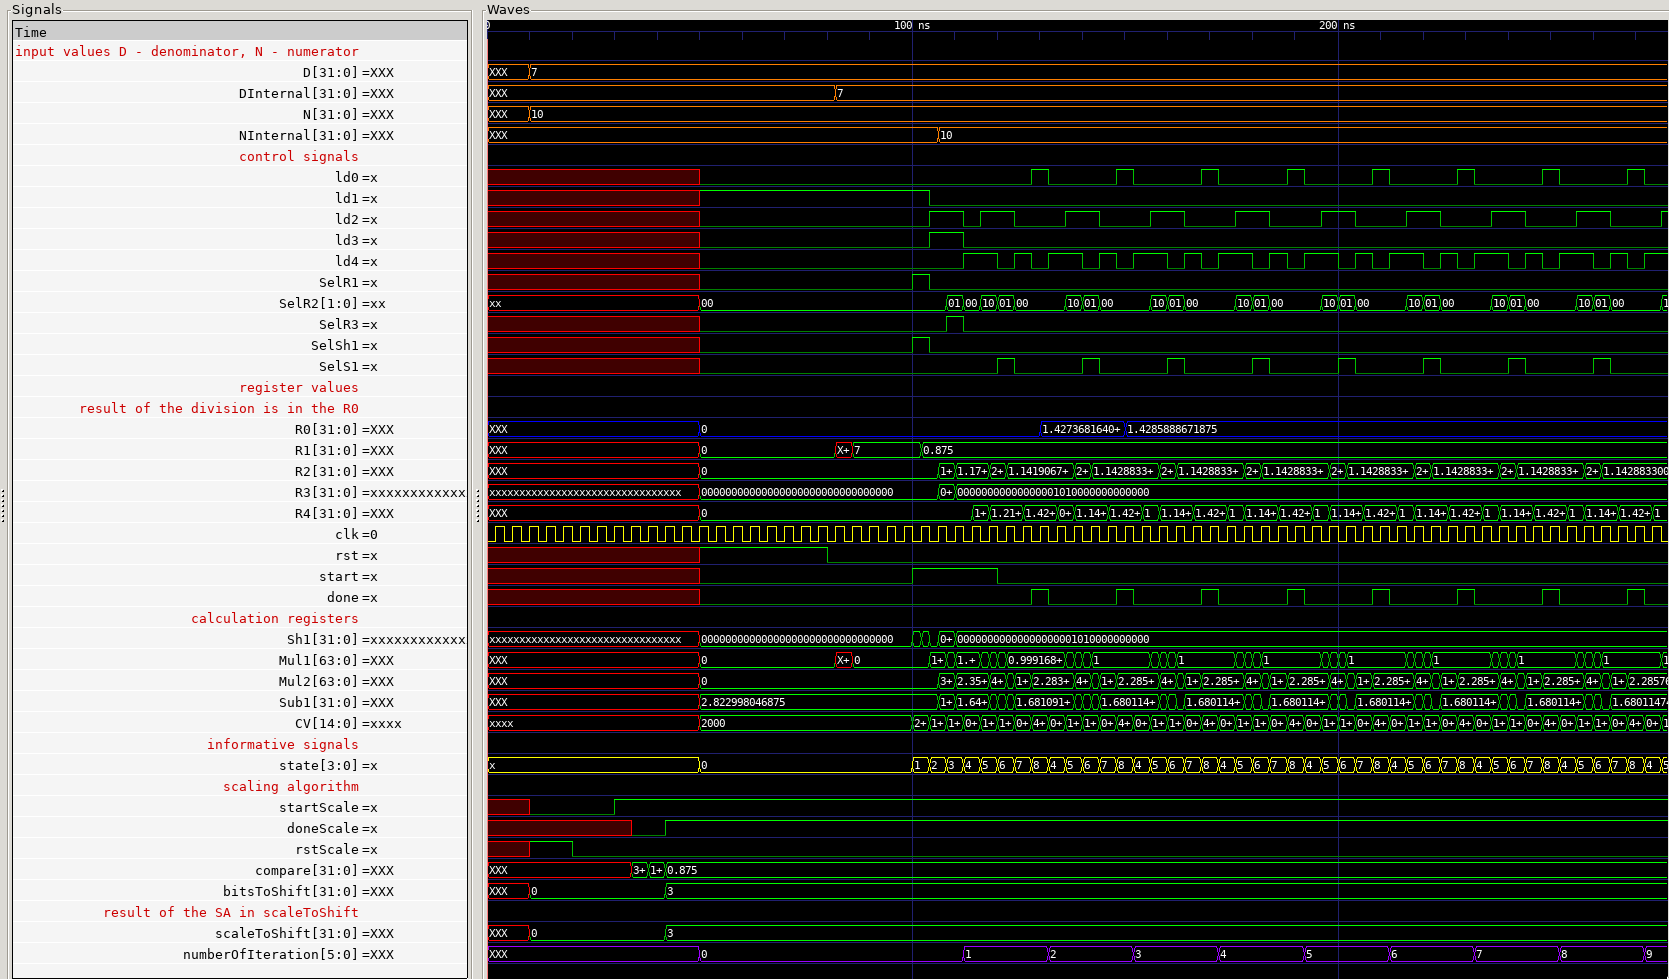
\includegraphics[width=1\textwidth]{src/png/division-10-div-7.png}
    \caption{Selected signals from simulation of division N/D = 10 / 7. The correct result in \textit{R0} is obtained after two iterations (reg numberOfIterations).}
  \label{fig:division-10-div-7}
\end{figure}


\begin{figure}[htbp!]
  \centering
  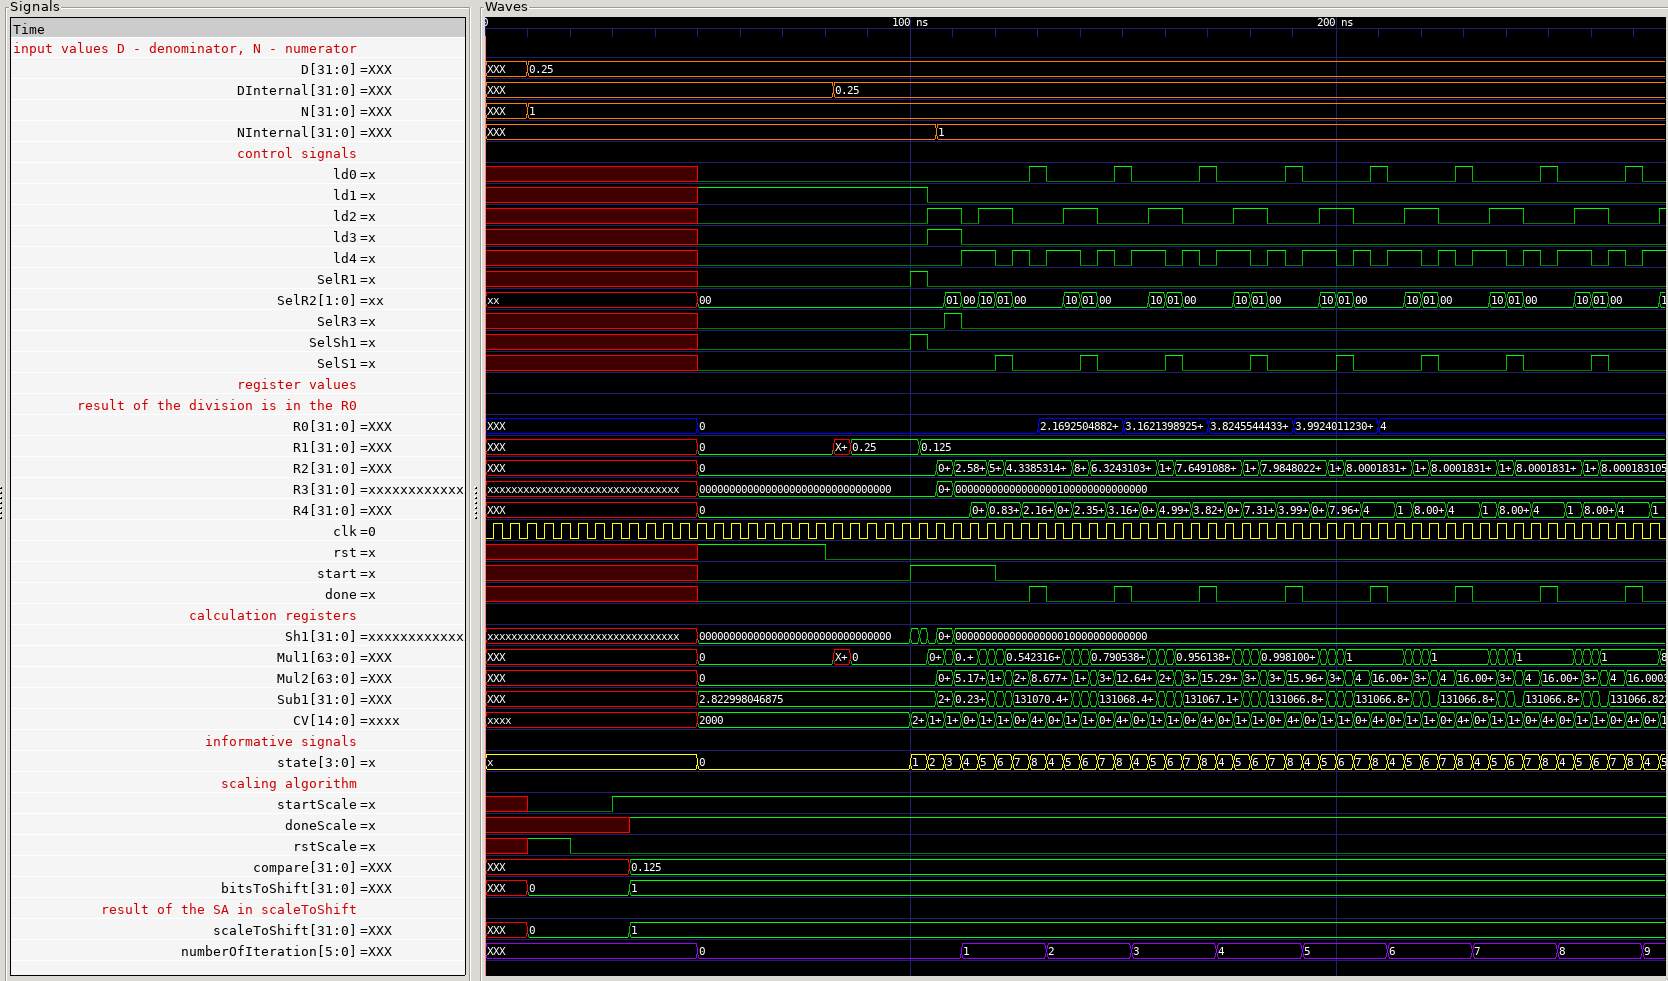
\includegraphics[width=1\textwidth]{src/png/division-1-div-0-25.png}
   \caption{Selected signals from simulation of division N/D = 1 / 0.25. The correct result in \textit{R0} is obtained after five iterations (reg numberOfIterations).}
  \label{fig:division-1-div-0-25}
\end{figure}

\begin{figure}[htbp!]
  \centering
  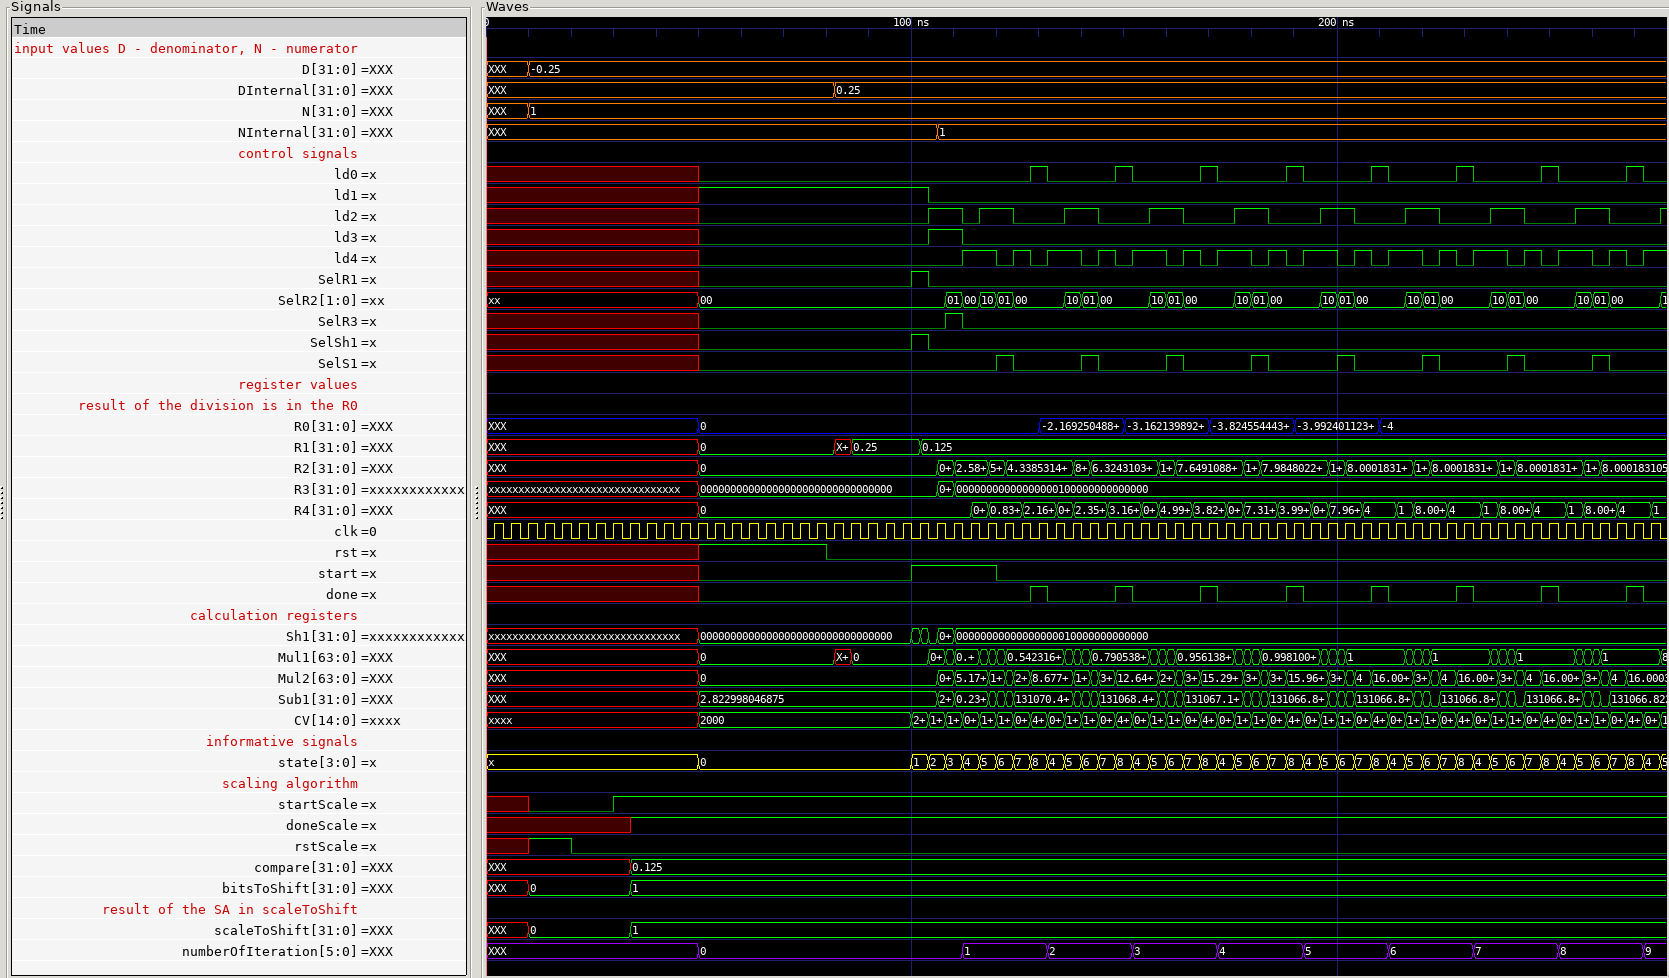
\includegraphics[width=1\textwidth]{src/png/division-1-div-minus-0-25.png}
    \caption{Selected signals from simulation of division N/D = 1 / (-0.25). The correct result in \textit{R0} is obtained after five iterations (reg numberOfIterations).}
  \label{fig:division-1-div-minus-0-25}
\end{figure}


\begin{figure}[htbp!]
  \centering
  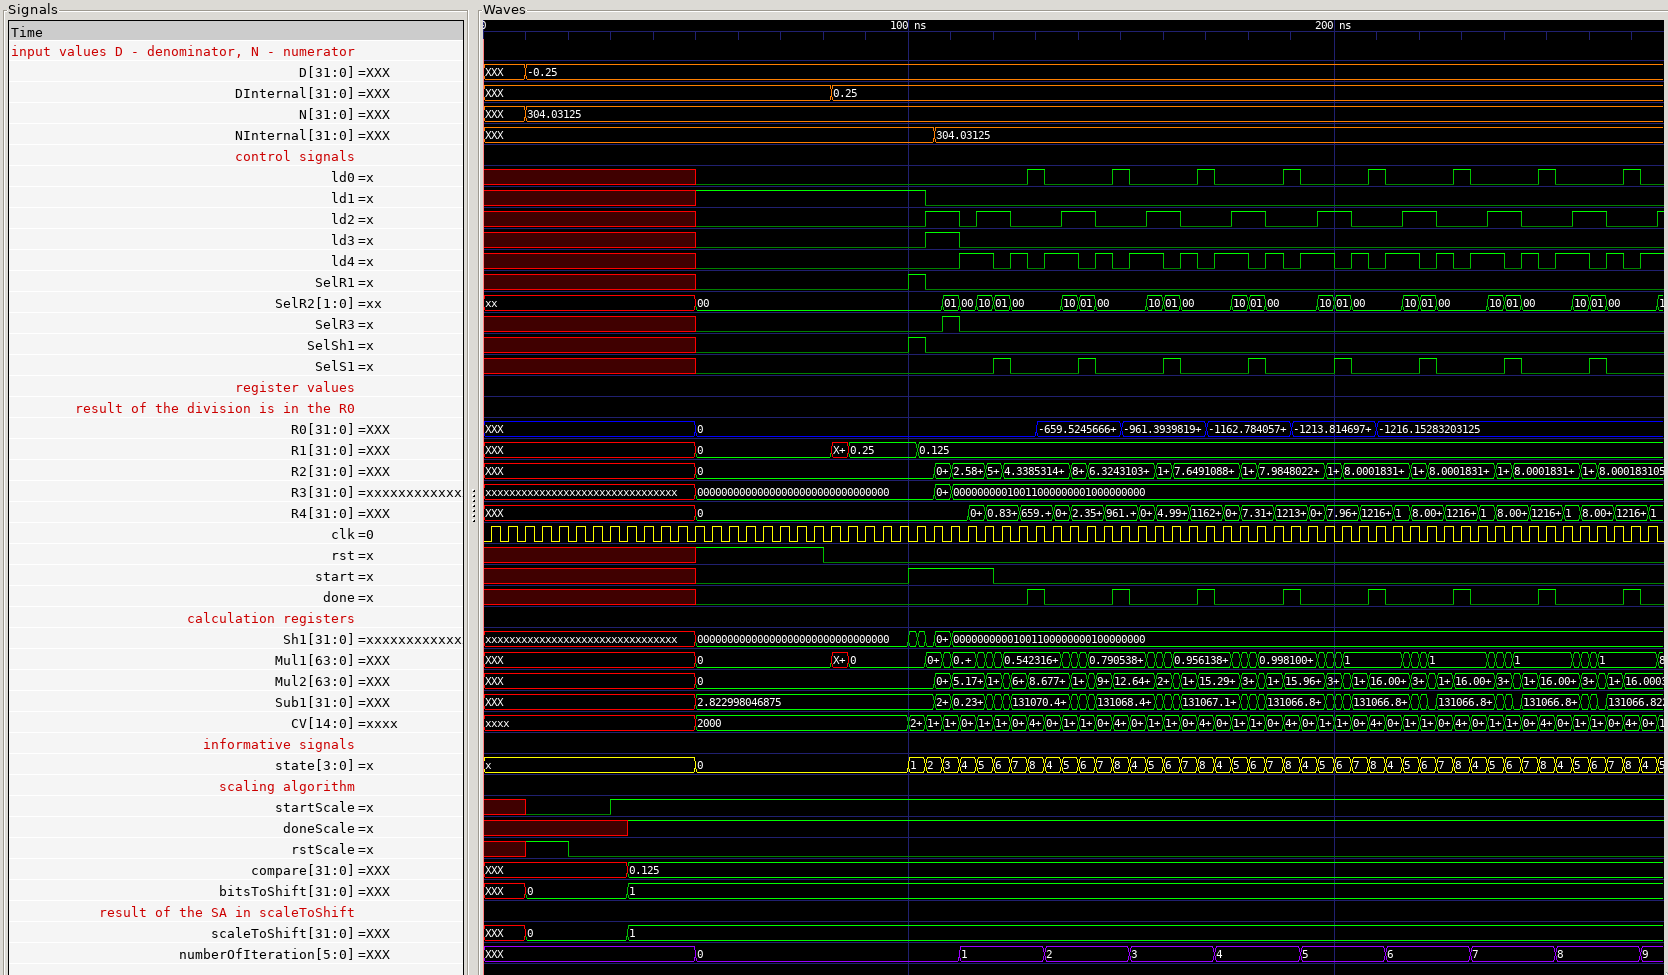
\includegraphics[width=1\textwidth]{src/png/division-304-03215-div-min-0-25.png}
    \caption{Selected signals from simulation of division N/D = 304.03215 / (-0.25). The correct result in \textit{R0} is obtained after five iterations (reg numberOfIterations).}
  \label{fig:division-304-03215-div-min-0-25}
\end{figure}

\begin{figure}[htbp!]
  \centering
  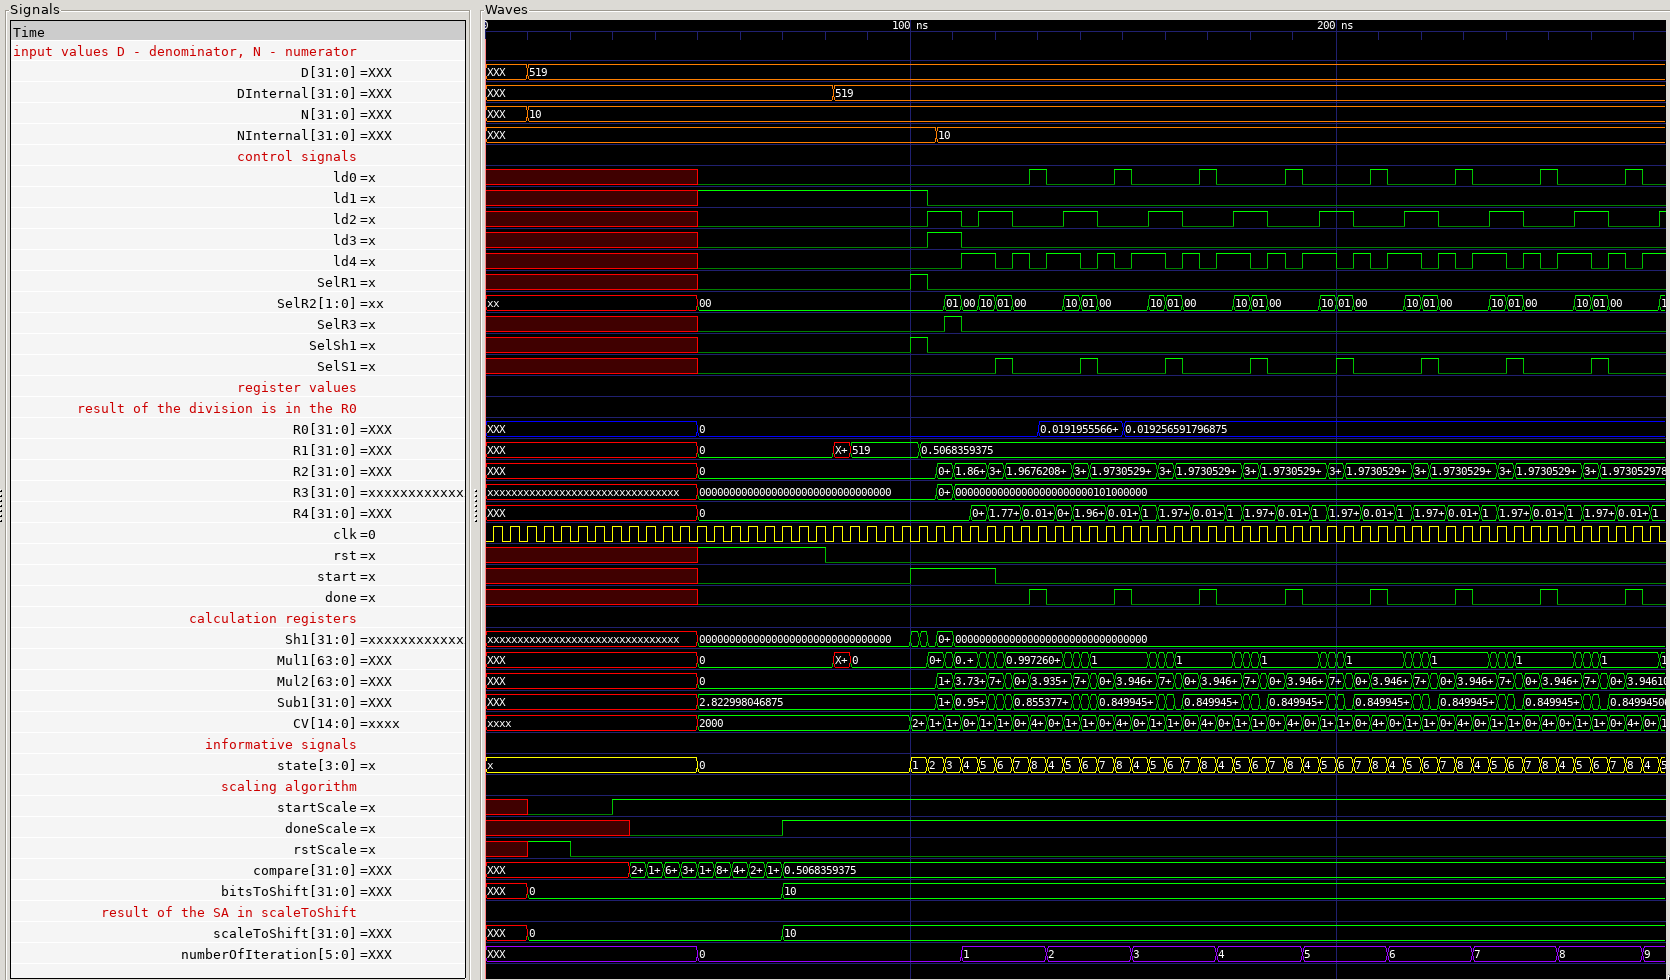
\includegraphics[width=1\textwidth]{src/png/division-10-div-519.png}
    \caption{Selected signals from simulation of division N/D = 10 / (519). The correct result in \textit{R0} is obtained after two iterations (reg numberOfIterations).}
  \label{fig:division-10-div-519}
\end{figure}

\section{Using CORDIC to calculate trigonometric functions}\label{sec:using-cordic-to-calculate-trigonometric-functions}
    There are numerous methods calculating trigonometric functions. To enhance flexibility, the Coordinate Rotation Digital Computer (\gls{abbreviation:cordic}) was selected over the Look-Up Table (\gls{abbreviation:lut}) implementation.\par
    While the \gls{abbreviation:lut} method may be fast, its accuracy depends on the size of the table. In contrast, when using the \gls{abbreviation:cordic} the precision depends on number of performed iterations of the algorithm. The modified algorithm is versatile and may be used to calculate non-trivial functions, including hyperbolic functions, square roots, multiplications, divisions, exponentials and logarithms. \cite{base-digital-signal-processing-with-field-programmable-gate-arrays} In this work only the calculation of $sinus$ and $cosinus$ functions is used.
    \subsection{Theory}\label{subsec:cordic-theory}
        The theory of the first \gls{abbreviation:cordic} was introduced by Volder in \cite{volder-cordic-trigonomtric-computing-technique}. This algorithm computes a coordinate conversion between rectangular ($x$, $y$) and polar ($R$, $\theta$) coordinates. The algorithm was then extended by Walther in \cite{walther-a-unified-algorithm-for-elementary-functions} to include circular, linear and hyperbolic transforms.  In this paper, only circular transforms are employed to calculate  $sine$ and $cosine$ functions. The presentation will focus on the fundamental aspects of the algorithm.\par
        The rotation of a vector in the rectangular coordinate system ($x$, $y$) may be described by matrix-vector multiplication depicted in the Equation \ref{eq:rotation}.

        \begin{equation}\label{eq:rotation}
             \begin{pmatrix}
                 x_\text{R}\\
                 y_\text{R}
             \end{pmatrix}
             =
             \begin{pmatrix}
                 \cos (\theta) & -\sin (\theta)\\
                 \sin (\theta) & \cos (\theta)
             \end{pmatrix}
             \begin{pmatrix}
                 x_\text{in}\\
                 y_\text{in}
             \end{pmatrix},
        \end{equation}

        where $x_\text{R}$ and $y_\text{R}$ are coordinates of a rotated vector, $\theta$ is the angle for which the vector with coordinates $x_\text{in}$ and $y_\text{in}$ was rotated.\par
        Then when simplifying the Equation \ref{eq:rotation}


        \begin{equation}\label{eq:rotation-simplifying}
             \begin{pmatrix}
                 x_\text{R}\\
                 y_\text{R}
             \end{pmatrix}
             = \cos (\theta)
             \begin{pmatrix}
                 1 & -\tan (\theta)\\
                 \tan (\theta) & 1
             \end{pmatrix}
             \begin{pmatrix}
                 x_\text{in}\\
                 y_\text{in}
             \end{pmatrix}
        \end{equation}

        \noindent it can be seen, that only multiplication by scaling factor of precalculated values of $\cos (\theta)$, multiplication by $\tan (\theta)$, subtraction and addiction operations are needed to perform the rotation. However, the multiplication by $\tan (\theta)$ can be replaced. The replacement may be done for angles $\theta$ for which the equation \ref{eq:tan-theta-2} is true. When implementing the algorithm to the \gls{abbreviation:fpga} the multiplication may be swapped for signed right bit shift, which is faster operation than multiplication.

        \begin{equation}\label{eq:tan-theta-2}
            \tan (\theta) = 2^{-1}.
        \end{equation}
        \par
        When the values $x_\text{in} = 1$ and $y_\text{in} = 0$ are used, the result for $sine$ and $cosine$ may be easily obtained from $x_\text{R}$ and $y_\text{R}$ as expressed in the Equation \ref{eq:xr-yr-when-initial-values-1-0}.

        \begin{equation}\label{eq:xr-yr-when-initial-values-1-0}
            \begin{gathered}
            x_\text{R} = x_\text{in} \cos (\theta) - y_\text{in} \sin (\theta) = | \theta = 0 | = \cos (\theta),\\
            y_\text{R} = x_\text{in} \sin (\theta) + y_\text{in} \cos (\theta) = | \theta = 0 | = \sin (\theta).
            \end{gathered}
        \end{equation}

            The algorithm can be further simplified by assuming that it is designed to undergo more than 6 iterations and thus the scaling constant, represented by multipliying $cosine$ of different $\theta$ values, converges to $0,60725$. If this condition is true, there is no necessity to precalculate all the scaling values and only the convergenent value may be used for the multiplication. In this paper the precalculated values are passed from the custom \gls{abbreviation:lut} module to the main algorithm.\par
            As evident from the \hyperref[subsubsec:example-of-calculation]{\textit{Example of calculation}} section or the algorithm theory itself, it is essential to estabilish whether the angle for which the vector is rotated in the next iteration should be in a positive direction (counter-clockwise) or negative direction (clockwise). To address this, the set of the equations is expanded, and new variable $z_i$ is introduced. The complete set of equations utilized in the implementation is as follows.

            \begin{equation}
                \begin{gathered}
                x [i+1] = x [i] - \sigma_i 2^{-i} y[i],\\
                y [i+1] = y [i] + \sigma_i 2^{-i} x[i],\\
                z~[i+1] = z~[i] - \sigma_i \atan (2^{-i}).
                \end{gathered}
            \end{equation}
            The $\sigma_{i+1}$ is determined based on the sign of the $z_{i+1}$ variable

            \begin{equation}
                \sigma_{i+1} = 
                \left\{
                \begin{array}{lr}
                    -1,\;\text{if}\;z_{i+1} < 0\\
                    1,\;\text{if}\;z_{i+1} > 0\\
                    0,\;\text{if}\;z_{i+1} = 0
                \end{array}
                \right\}
            \end{equation}
            \par
            The algorithm, as presented, accurately computes values for $sine$ and $cosine$ functions only in the first and fourth quadrants ($3\pi/2$ to $\pi/2$ counter-clockwise). To expand its applicability across the entire $2\pi$ range, specific actions must be taken before the actual looped aglorithm.\par
            The algorithm must determine the quadrant, where the desired angle $\theta$ for which the $sine$ and $cosine$ functions are to be calculated is. This determination is made through \texttt{if} statements during the initialization of the algorithm values and at the final value calculation. If the reference angle $\theta$ falls outside the first or fourth quadrant, then the angle is rotated from its original quadrant to either the first or fourth quadrant. Depending on the quadrant, to which the angle is rotated, the $\sigma_i$ value is set accordingly. The corresponding if statements during the algorithm initialization are provided in Pseudocode \ref{lst:cordic-initial-if-statements}. Similar statements used at the final values calculation are presented in Pseudocode \ref{lst:cordic-ending-if-statements}.\par
            The pseudocodes use \texttt{initialZValue} as a reference angle $\theta$, for which to calculate the $sine$ and $cosine$ function values, \texttt{zValue} as a temporary value for calculating the iterations for $z_{i}$ variables, \texttt{sigmaValue} for temporary value holding the current iteration value of $\sigma_i$, the \texttt{resultCos} and \texttt{resultSin} variables are used for storing the temporary and final values of the $\cos (\theta)$ and $\sin (\theta)$ values respectively.

\begin{lstlisting}[language={pseudocode}, caption={Pseudocode for if statements used at the value initialization of the \gls{abbreviation:cordic} algorithm.}, label= {lst:cordic-initial-if-statements}]
if((initialZValue > 1.5707)&(initialZValue < 3.141592))
    sigmaValue = -1
    zValue = initialZValue - 3.141592
else if((initialZValue > 3.141592)&(initialZValue < 4.7123))
    sigmaValue = 1
    zValue = initialZValue - 3.141592
else
    zValue = initialZValue
    sigmaValue = 1
end
\end{lstlisting}


\begin{lstlisting}[language={pseudocode}, caption={Pseudocode for if statements used at the final $sinus$ and $cosinus$ value calculation.}, label= {lst:cordic-ending-if-statements}]
if((initialZValue > 1.5707)&(initialZValue < 3.141592))
    resultCos = - resultCos
    resultSin = resultSin
else if((initialZValue > 3.141592)&(initialZValue < 4.7123))
    resultCos = - resultCos
    resultSin = - resultSin
end
\end{lstlisting}

        \subsubsection{Example of calculation}\label{subsubsec:example-of-calculation}
            The \gls{abbreviation:cordic} algorithm's general approach can be illustrated by calculating the $sine$ and $cosine$ values for the reference angle $\theta = 57,535\;˚$. Initially, the angle is deconstructed into its base angles, satisfying the Equation \ref{eq:tan-theta-2}. In this example the deconstruction is $57,535 = 45 + 25,565 -14,03$.\par
            The index $i$ of the variables $x_i$ and $y_i$ in the following equations means the number of iteration of the algorithm.

            \begin{equation}
                0.\;\text{iteration}\;
                \begin{pmatrix}
                    x_0\\y_0
                \end{pmatrix}
                =
                \cos (45\;°)
                \begin{pmatrix}
                    1 & -1\\
                    1 & 1
                \end{pmatrix}
                \begin{pmatrix}
                    x_\text{in}\\
                    y_\text{in}
                \end{pmatrix},
            \end{equation}

            
            \begin{equation}
                1.\;\text{iteration}\;
                \begin{pmatrix}
                    x_1\\y_1
                \end{pmatrix}
                =
                \cos (26,565\;°)
                \begin{pmatrix}
                    1 & -2^{-1}\\
                    2^{-1} & 1
                \end{pmatrix}
                \begin{pmatrix}
                    x_0\\
                    y_0
                \end{pmatrix},
            \end{equation}


            \begin{equation}
                2.\;\text{iteration}\;
                \begin{pmatrix}
                    x_2\\y_2
                \end{pmatrix}
                =
                \cos (-14,03\;°)
                \begin{pmatrix}
                    1 & -2^{-2}\\
                    2^{-2} & 1
                \end{pmatrix}
                \begin{pmatrix}
                    x_1\\
                    y_1
                \end{pmatrix}.
            \end{equation}

            Then values $x_2$ and $y_2$ may be obtained.\par
            \begin{equation}\label{eq:example-cordic-calculation}
                \begin{pmatrix}
                    x_2\\y_2
                \end{pmatrix}
                =
                \cos (45\;°)
                \cos (25,565\;°)
                \cos (-14,03\;°)
                \begin{pmatrix}
                    1 & -2^{-2}\\
                    2^{-2} & 1
                \end{pmatrix}
                \begin{pmatrix}
                    1 & -2^{-1}\\
                    2^{-1} & 1
                \end{pmatrix}
                \begin{pmatrix}
                    1 & -1\\
                    1 & 1
                \end{pmatrix}
                \begin{pmatrix}
                    x_\text{in}\\
                    y_\text{in}
                \end{pmatrix}.
            \end{equation}

            \par
             The values $x_2$ and $y_2$ in the Equation \ref{eq:example-cordic-calculation} correspond to $\cos (57,535\;˚)$ and $\sin (57,535\;˚)$ respectively.

    \subsection{Python Implementation}\label{subsec:cordic-python-implementation}
        For simplicity, the \gls{abbreviation:cordic} algorithm was prototyped in Python. This proved highly beneficial, as the debugging of the Python code is much more straightforward compared to debugging Verilog design without prepared and debugged algoritm in a higher level language.\par
        The Python code was used to precalculate the \gls{abbreviation:lut} for scaling factor and arcus tangens values for $z_i$ calculations.\par
        For clarity, the Python implementation is provided in Code \ref{lst:python-cordic}. The presented Code also calculates the error between the \gls{abbreviation:cordic}-calculated value and the Python math library functions.

\begin{lstlisting}[language={python}, caption={Python code of \gls{abbreviation:cordic} implementation.}, label= {lst:python-cordic}]
import math

# Defining starting values and empty arrays
totalNumberOfIterations = 12 # 12 - best tradeof between value and iterations
atanValues = []
scalingValues = [1]
initialXValueCordic = 1
initialYValueCordic = 0
# initialZValueCordic = 1.248  # angle for which to calculate cordic
# initialZValueCordic = - 1.248  # angle for which to calculate cordic
# initialZValueCordic = - 6.7194  # angle for which to calculate cordic
initialZValueCordic = 10.7194824  # angle for which to calculate cordic
initialSigmaValueCordic = 1

for x in range(totalNumberOfIterations):
    # Generating arcus tanges values of precalculated angles based on number of iterations
    atanValues.append(math.atan(1*2**(-x)))
    # Generating precalculated scaling values based on a number of iterations
    scalingValues.append(scalingValues[x]*math.cos(atanValues[x]))

print("atanValues: ", atanValues)
print("scalingValues: ", scalingValues)

print("*-+-+-+-+-+-+-+-+-+-+-+-+-+-+-+-+-+-+-+-+-+-+-+-+-+-+-*")
print("\n")
print("initialZValue original: ", initialZValueCordic)

# Moving angle to interval [0,2Pi]
if initialZValueCordic > 0:
    while initialZValueCordic > (2*3.141592):
        initialZValueCordic = initialZValueCordic - 2*3.141592
else:
    while initialZValueCordic < (-2*3.141592):
        initialZValueCordic = initialZValueCordic + 2*3.141592


print("initialZValue after moving to [0,2Pi] interval: ", initialZValueCordic)
print("\n")
print("*-+-+-+-+-+-+-+-+-+-+-+-+-+-+-+-+-+-+-+-+-+-+-+-+-+-+-*")

# Checking the initial value and moving it in the interval
if (initialZValueCordic > 1.5707) and (initialZValueCordic < 3.141592):
    zValue = initialZValueCordic - 3.141592
    sigmaValue = -1
    print("value in second q")
elif (initialZValueCordic > 3.141592) and (initialZValueCordic < 4.7123):
    zValue = initialZValueCordic - 3.141592
    sigmaValue = 1
    print("value in third q")
elif (initialZValueCordic < 0):
    sigmaValue = -1
    zValue = initialZValueCordic
    print("value in fourth q")
else:
    zValue = initialZValueCordic  # For angle
    sigmaValue = initialSigmaValueCordic  # For +- next angle
    print("value in first")

# Passing starting values to the calculation values
xValue = initialXValueCordic  # For cos
yValue = initialYValueCordic  # For sin


# CORDIC ALGORITHM
for x in range(totalNumberOfIterations):

    # Calculating next values of the current iteration x
    xNextValue = xValue - (sigmaValue*yValue)*2**(-x)
    yNextValue = yValue + (sigmaValue*xValue)*2**(-x)
    zNextValue = zValue - sigmaValue * atanValues[x]

    # Determining the signum of next angle (addition or subtraction)
    if zNextValue >= 0:
        sigmaNextValue = 1
    else:
        sigmaNextValue = -1

    # Values for new iteration
    xValue = xNextValue
    yValue = yNextValue
    zValue = zNextValue
    sigmaValue = sigmaNextValue

    print("iteration:", x, "xValue:", xValue, "yValue:", yValue, "zValue:", zValue, "sigmaValue:", sigmaValue, "\n")

# Calculating results by scaling the result values from CORDIC by the scalingValue which depends on number of iterations which were made
resultCos = scalingValues[x-1] * xValue
resultSin = scalingValues[x-1] * yValue

# Changing results sign based on the rotation of the initialZValueCordic
if (initialZValueCordic > 1.5707) and (initialZValueCordic < 3.141592):
    resultCos = - resultCos
elif (initialZValueCordic > 3.141592) and (initialZValueCordic < 4.7123):
    resultCos = - resultCos
    resultSin = - resultSin

# Calculating values based on the math library
mathResultCos = math.cos(initialZValueCordic)
mathResultSin = math.sin(initialZValueCordic)

# Calculating the error of CORDIC calculated values from the python math functions
errorCos = abs(resultCos) - abs(mathResultCos)
errorSin = abs(resultSin) - abs(mathResultSin)

# Results printing
print("*-+-+-+-+-+-+-+-+-+-+-+-+-+-+-+-+-+-+-+-+-+-+-+-+-+-+-*")
print("CORDIC results:")
print("cos: ", resultCos)
print("sin: ", resultSin)
print("scaleFactor: ", scalingValues[totalNumberOfIterations-1])
print("\n")
print("MATH results:")
print("cos: ", mathResultCos)
print("sin: ", mathResultSin)
print("\n")
print("error CORDIC-MATH:")
print("cos: ", errorCos)
print("sin: ", errorSin)
\end{lstlisting}

\par
Once the Python implementation and debugging are completed, the Verilog implementation of the algorithm can initiated. Similar to the Division Unit module, as presented in \hyperref[sec:calculating-the-division-of-fixed-point-numbers]{\textit{Calculating the division of fixed point numbers}} section, the Data Path, Control Unit and Top Module were designed. This application-specific circuit design approach should be faster and safer than creating a custom \gls{abbreviation:cpu} with reduced and customized \gls{abbreviation:isa}.

    \fbar
    \subsection{IP Block Design}
    \fbar
        \subsubsection{Top module design}
            The top module design of the \gls{abbreviation:cordic} \gls{abbreviation:ip} is illustrated in Figure \ref{fig:cordic-top-module}. As evident, the structure closely resembles that of the Division Unit top module. When using an approach to create a customized circuit for an algorithm, the process of developing the top modules is likely to be similar, with minor differences in signals, inputs and variables.\par
            The Data Path module incorporates precalculated values in \gls{abbreviation:lut}s for \textit{atanValues} and \textit{scalingValues}. In this implementation, the value of \textit{totalNumberOfIterations} is set to 12 , making the \gls{abbreviation:lut} 12x32 bits in size. It is worth noting that the previously introduced custom fixed-point format \textit{Q32.15} is utilized.
            \begin{figure}[htbp!]
                \centering
                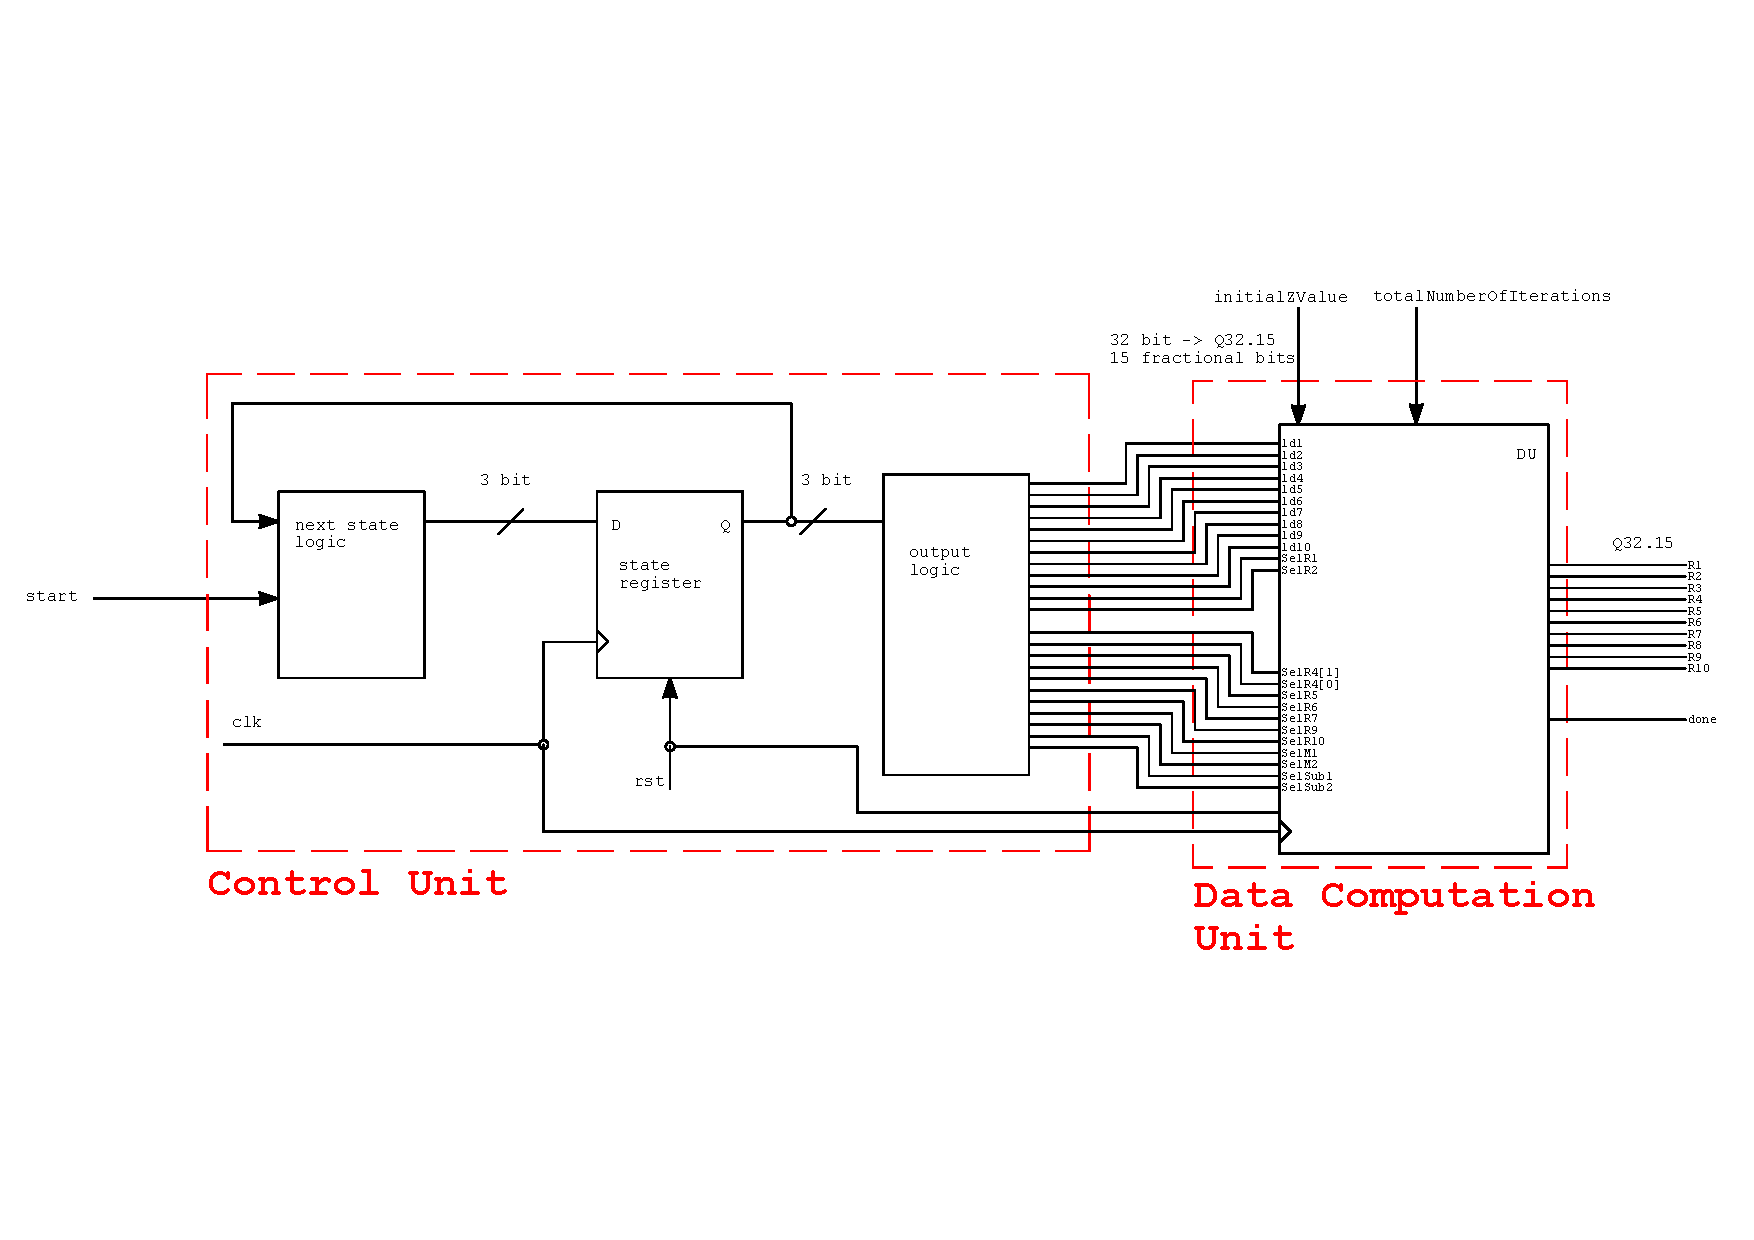
\includegraphics[width=1\textwidth]{src/pdf/cordic-top-module.pdf}
                \caption{Top module design for the \gls{abbreviation:cordic} module block design.}
                \label{fig:cordic-top-module}
            \end{figure}
        \fbar
        \subsubsection{Allocation and Timing}
            In Figure \ref{fig:cordic-allocation-timing}, the allocation and timing diagram is depicted. Notably, the if statements, implemented in the control unit, are documented within the diagram. The explanation, why the if statements are needed, is presented in the \gls{abbreviation:cordic} \hyperref[subsec:cordic-theory]{\textit{Theory}} section.\par
            As mentioned in the \gls{abbreviation:cordic} \hyperref[subsubsec:cordic-control-unit]{\textit{Control Unit}} sections, there are two primary approaches to iteration cycles. The one is to proceed from \textit{S4} to \textit{S2} for a faster algorithm, while the other involves progressing from \textit{S6} to \textit{S2}. The latter approach is employed for demonstrative purposes, as it ensures that the final numerical values are always calculated.
            \begin{figure}[htbp!]
                \centering
                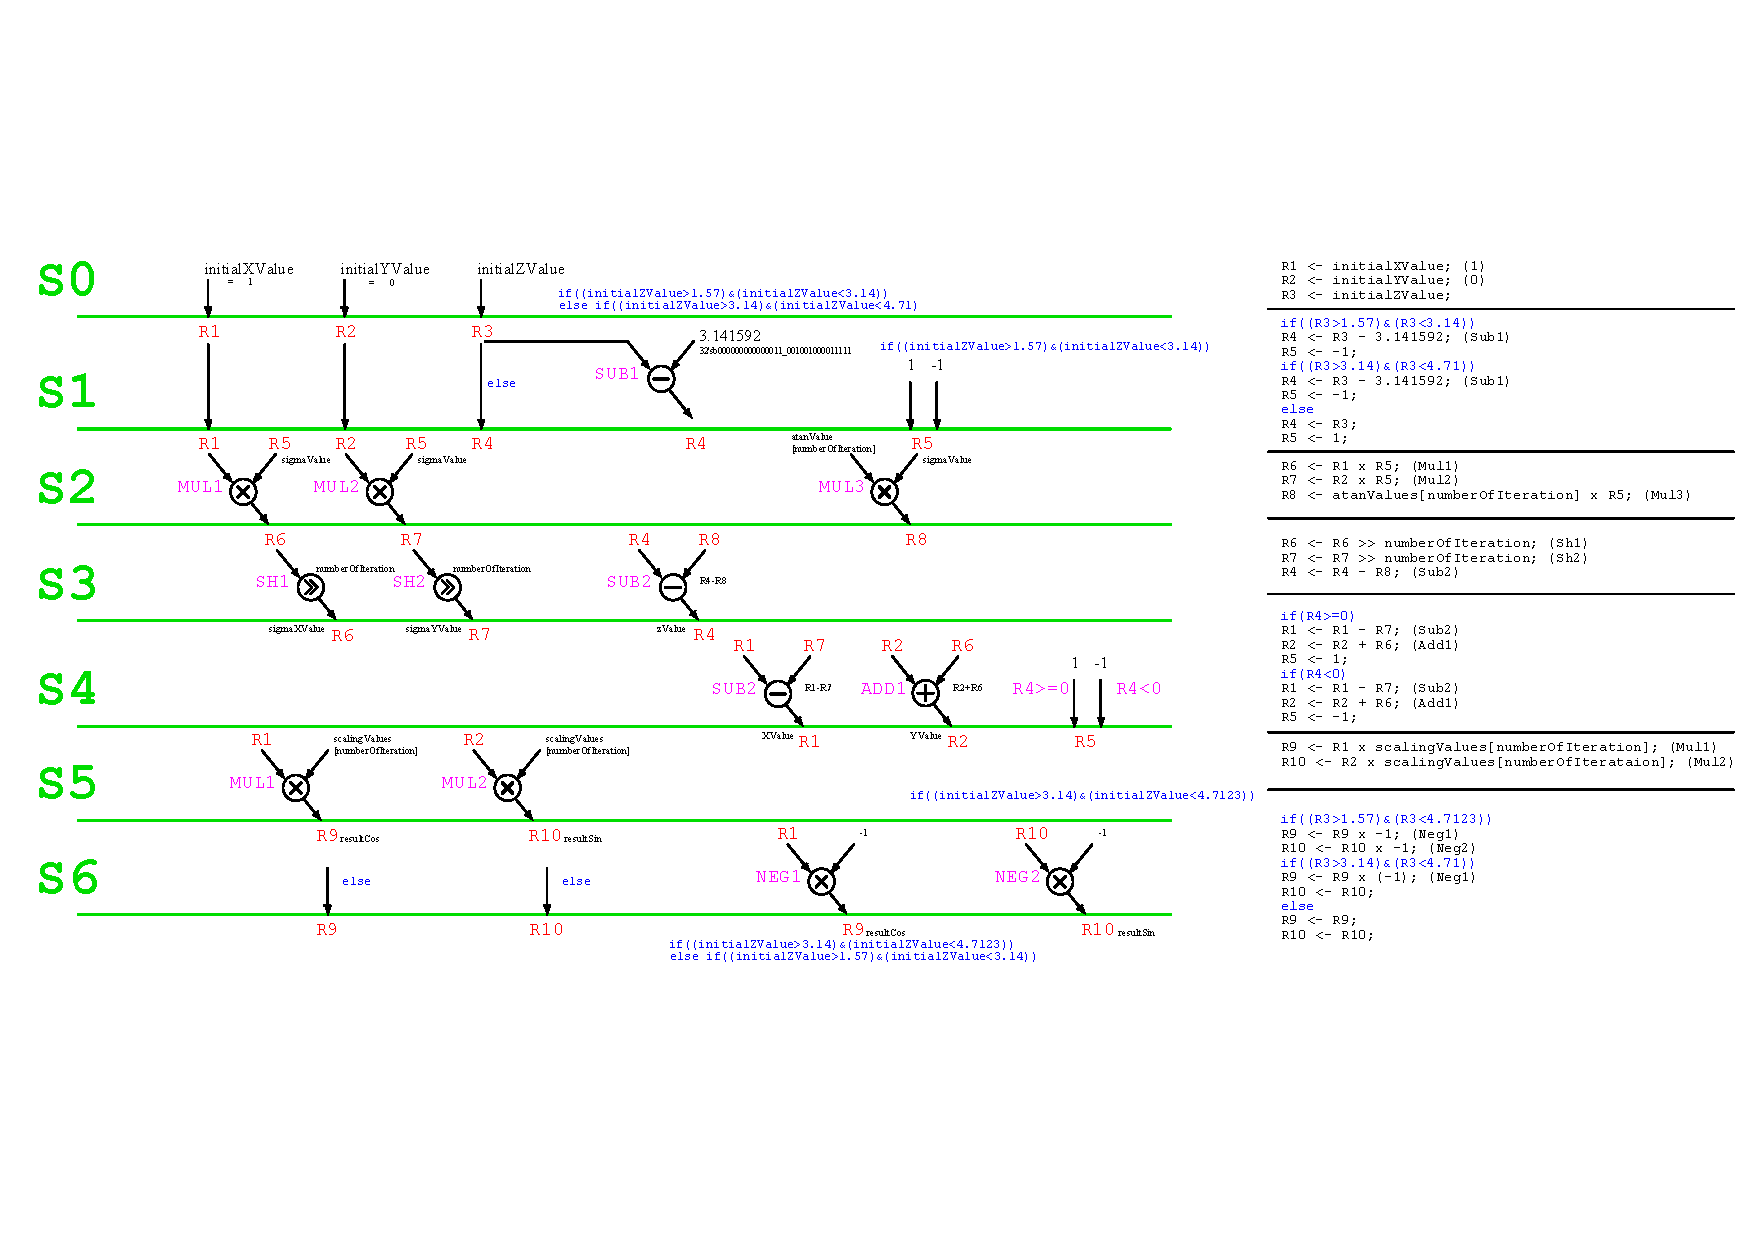
\includegraphics[width=1\textwidth]{src/pdf/cordic-allocation-timing.pdf}
                \caption{Alloccation and timing diagram for the Data Path Unit part of the \gls{abbreviation:cordic} \gls{abbreviation:ip}.}
                \label{fig:cordic-allocation-timing}
            \end{figure}
        \fbar
        \subsubsection{Data Path Module}
            The Figure \ref{fig:cordic-rtl} presents the Data Path module of the design, calculation and storing units included. The memory \gls{abbreviation:lut}s for \textit{atanValues} and \textit{scalingValues} are presented not as separate registers but as inputs to the calculation unit. The results of $sine$ and $cosine$ functions, referred to as \textit{resultSin} and \textit{resultCos} in the Python implementation, are stored to registers R9 and R10, respectively. It is important to note that the \textbf{NEG} blocks are not implemented as calculation unit blocks for generating the negative numbers. Instead negation is activated in the corresponding target register when the appropriate \textbf{SelR$_x$} is activated. (where $x$ represents the number of a corresponding register, either R9 or R10)\par
            The implementation of the \gls{abbreviation:lut} memory module for $atanValues$ is depicted in Code \ref{lst:atanValuesCordicLUT}, memory module for $scalingValues$ is depicted in Code \ref{lst:scalingValuesCordicLUT}.
            \begin{figure}[htbp!]
                \centering
                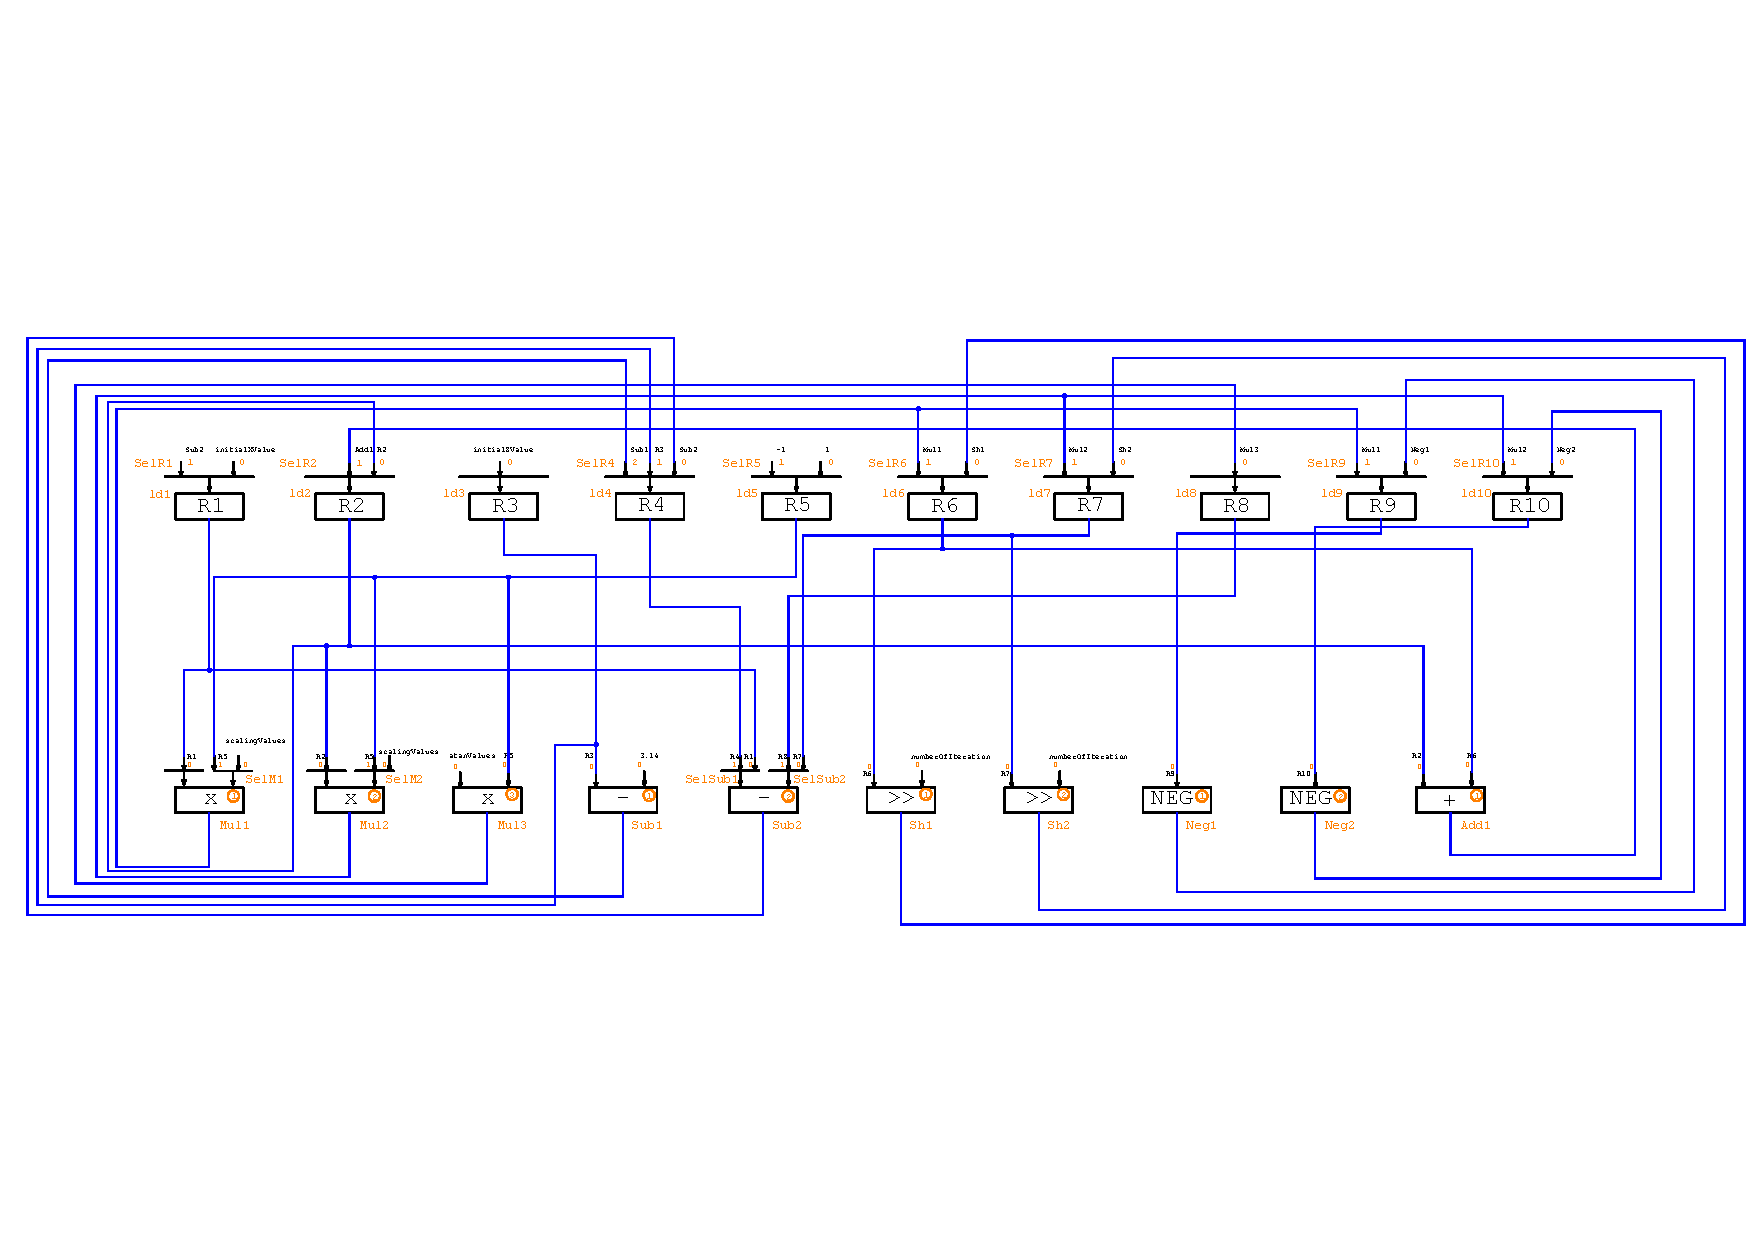
\includegraphics[width=1\textwidth]{src/pdf/cordic-rtl.pdf}
                \caption{Register transfer level (\gls{abbreviation:rtl}) scheme of the \gls{abbreviation:cordic} \gls{abbreviation:ip} Data Path Unit \gls{abbreviation:ip}.}
                \label{fig:cordic-rtl}
            \end{figure}
            
            \fbar
            \begin{lstlisting}[language={verilog}, caption={Verilog code of the atanValuesCordicLUT  lookup table (\gls{abbreviation:lut}) implementation.}, label= {lst:atanValuesCordicLUT}]
module atanValuesCordicLUT(index, returnValue);

input [3:0] index;
output reg signed [31:0] returnValue;


always@(index)
begin
    case(index)
        4'b0000: returnValue = 32'sb00000000000000000_110010010000111; // 0.7853981633974483
        4'b0001: returnValue = 32'sb00000000000000000_011101101011000; // 0.4636476090008061
        4'b0010: returnValue = 32'sb00000000000000000_001111101011011; // 0.24497866312686414
        4'b0011: returnValue = 32'sb00000000000000000_000111111101010; // 0.12435499454676144
        4'b0100: returnValue = 32'sb00000000000000000_000011111111101; // 0.06241880999595735
        4'b0101: returnValue = 32'sb00000000000000000_000001111111111; // 0.031239833430268277
        4'b0110: returnValue = 32'sb00000000000000000_000000111111111; // 0.015623728620476831
        4'b0111: returnValue = 32'sb00000000000000000_000000011111111; // 0.007812341060101111
        4'b1000: returnValue = 32'sb00000000000000000_000000001111111; // 0.007812341060101111
        4'b1001: returnValue = 32'sb00000000000000000_000000000111111; // 0.0019531225164788188
        4'b1010: returnValue = 32'sb00000000000000000_000000000011111; // 0.0009765621895593195
        4'b1011: returnValue = 32'sb00000000000000000_000000000001111; // 0.0004882812111948983
        default: returnValue = 32'sb00000000000000000_000000000000000; // 0
    endcase
end
endmodule\end{lstlisting}

            \begin{lstlisting}[language={verilog}, caption={Verilog code of the scalingValuesCordicLUT lookup table (\gls{abbreviation:lut}) implementation.}, label= {lst:scalingValuesCordicLUT}]
module scalingValuesCordicLUT(index, returnValue);

input [3:0] index;
output reg signed [31:0] returnValue;

always@(index)
begin
    case(index)
        4'b0000: returnValue <= 32'sb000000000000000001_000000000000000; // 1
        4'b0001: returnValue <= 32'sb00000000000000000_101101010000010; // 0.7071067811865476
        4'b0010: returnValue <= 32'sb00000000000000000_101000011110100; // 0.6324555320336759
        4'b0011: returnValue <= 32'sb00000000000000000_100111010001001; // 0.6135719910778964
        4'b0100: returnValue <= 32'sb00000000000000000_100110111101110; // 0.6088339125177524
        4'b0101: returnValue <= 32'sb00000000000000000_100110111000111; // 0.6088339125177524
        4'b0110: returnValue <= 32'sb00000000000000000_100110110111101; // 0.607351770141296
        4'b0111: returnValue <= 32'sb00000000000000000_100110110111011; // 0.6072776440935261
        4'b1000: returnValue <= 32'sb00000000000000000_100110110111010; // 0.6072591122988928
        4'b1001: returnValue <= 32'sb00000000000000000_100110110111010; // 0.6072544793325625
        4'b1010: returnValue <= 32'sb00000000000000000_100110110111010; // 0.6072533210898753
        4'b1011: returnValue <= 32'sb00000000000000000_100110110111010; // 0.6072530315291345
        default: returnValue <= 32'sb00000000000000000_000000000000000; // 0
    endcase
end
endmodule\end{lstlisting}
        \fbar
        \subsubsection{Control Unit}\label{subsubsec:cordic-control-unit}
        Similarly to the Division \hyperref[subsubsec:division-control-unit]{\textit{Control Unit}} section, the encoding of the control signal is presented in Table \ref{tab:control-signal-cordic-unit}.\par
        The branches of if statements used in the design have been color-coded to enhance clarity. Steps \textit{S5} and \textit{S6} are mainly focused on multiplying the result of iteration by the appropriate scaling value and on multiplying the calculated values based on the quadrant of the original reference angle value.
        \subfile{src/tex/cordic-control-unit-table.tex}
    \subsection{Simulation results}
    The testbench for testing the design was developed using Cocotb \cite{cocotb} with the Verilator \cite{verilator} as a simulator.\par
    It becomes evident during the algorithm implementation, where the actual iteration values for $sine$ and $cosine$ are calculated, that the number of cycles required for the final calculation can be determined as

    \begin{equation}
                NoCyc_\text{result every iteration} = 
                \left\{
                \begin{array}{lr}
                    3,\;\text{if}\;initialZValue \in [-2 \pi, 2 \pi]\\
                    4,\;\text{if}\;initialZValue \notin [-2 \pi, 2 \pi]
                \end{array}
                \right\}
         + \;5 NoIt,
    \end{equation}

    where $NoCyc$ (-) is the number of cycles and $NoIt$ is the number of iterations for the \gls{abbreviation:cordic} algorithm. The $4$ value is caused by states \textit{S0}-\textit{S4} and the multiplication by 5 is caused by states \textit{S4}–\textit{S8}. When the result of the \gls{abbreviation:cordic} algorithm is calculated only once at the end of the algorithm, the number of iterations can be determined by

    \begin{equation}
        NoCyc_\text{result at the end} = 
                \left\{
                \begin{array}{lr}
                    3,\;\text{if}\;initialZValue \in [-2 \pi, 2 \pi]\\
                    4,\;\text{if}\;initialZValue \notin [-2 \pi, 2 \pi]
                \end{array}
                \right\}
            +\;3 NoIt + 2,
    \end{equation}
    where the multiplication by value 3 is caused by states \textit{S4}–\textit{S6}, the addition of $4$ is caused by states \textit{S0}-\textit{S4} and the addition of the $2$ is casued by states \textit{S7}–\textit{S8}.\par
    \par
    In the simulation the $numberOfCycles$ displayed is an index of the cycle, so for angle $\theta = -1.247985$~rad is the number of iterations depicted on Figure \ref{fig:cordic-verilog-end-of-the-simulation} is $63$.

    The frequency of the clock signal in the simulation is currently set to 50 MHz.

        \begin{figure}[htbp!]
            \centering
            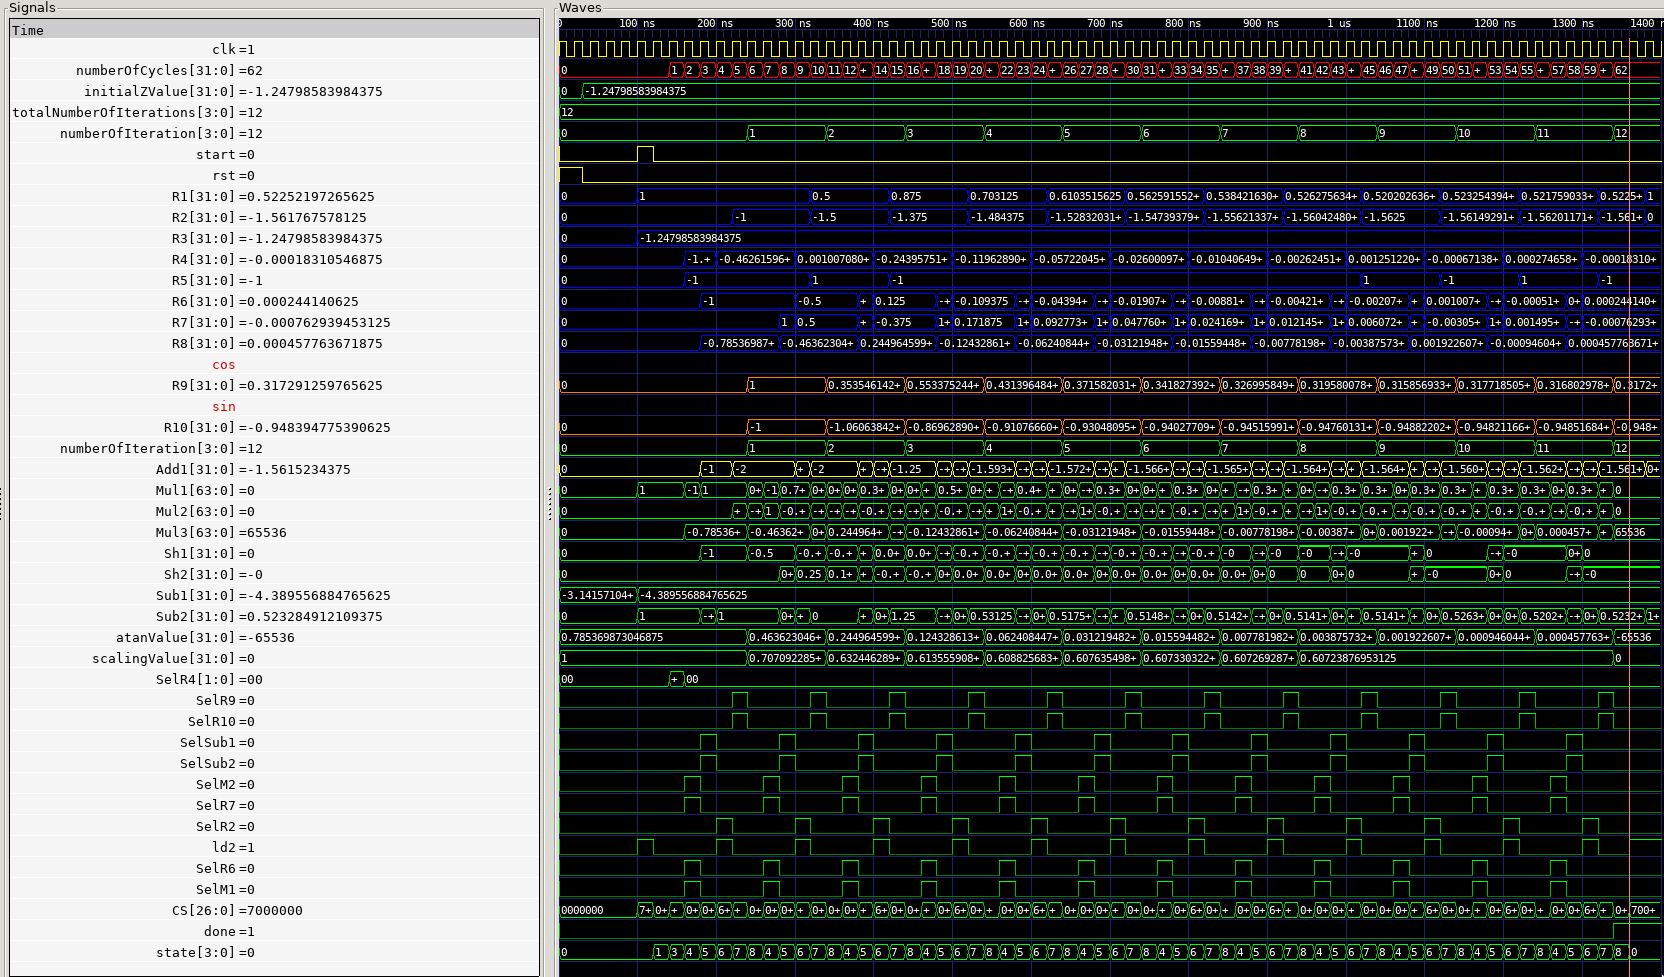
\includegraphics[width=1\textwidth]{src/png/cordic-verilog-whole-sim.png}
            \caption{The whole Verilog simulation of \gls{abbreviation:cordic} algorithm for determining the sine and cosine values of angle $\theta = -1.2479$ rad. The value of sine and cosine based on the current iteration is also calculated in this algorithm approach. The result is passed to the registers R9 and R10.}
            \label{fig:cordic-verilog-whole-sim}
        \end{figure}

        \begin{figure}[htbp!]
            \centering
            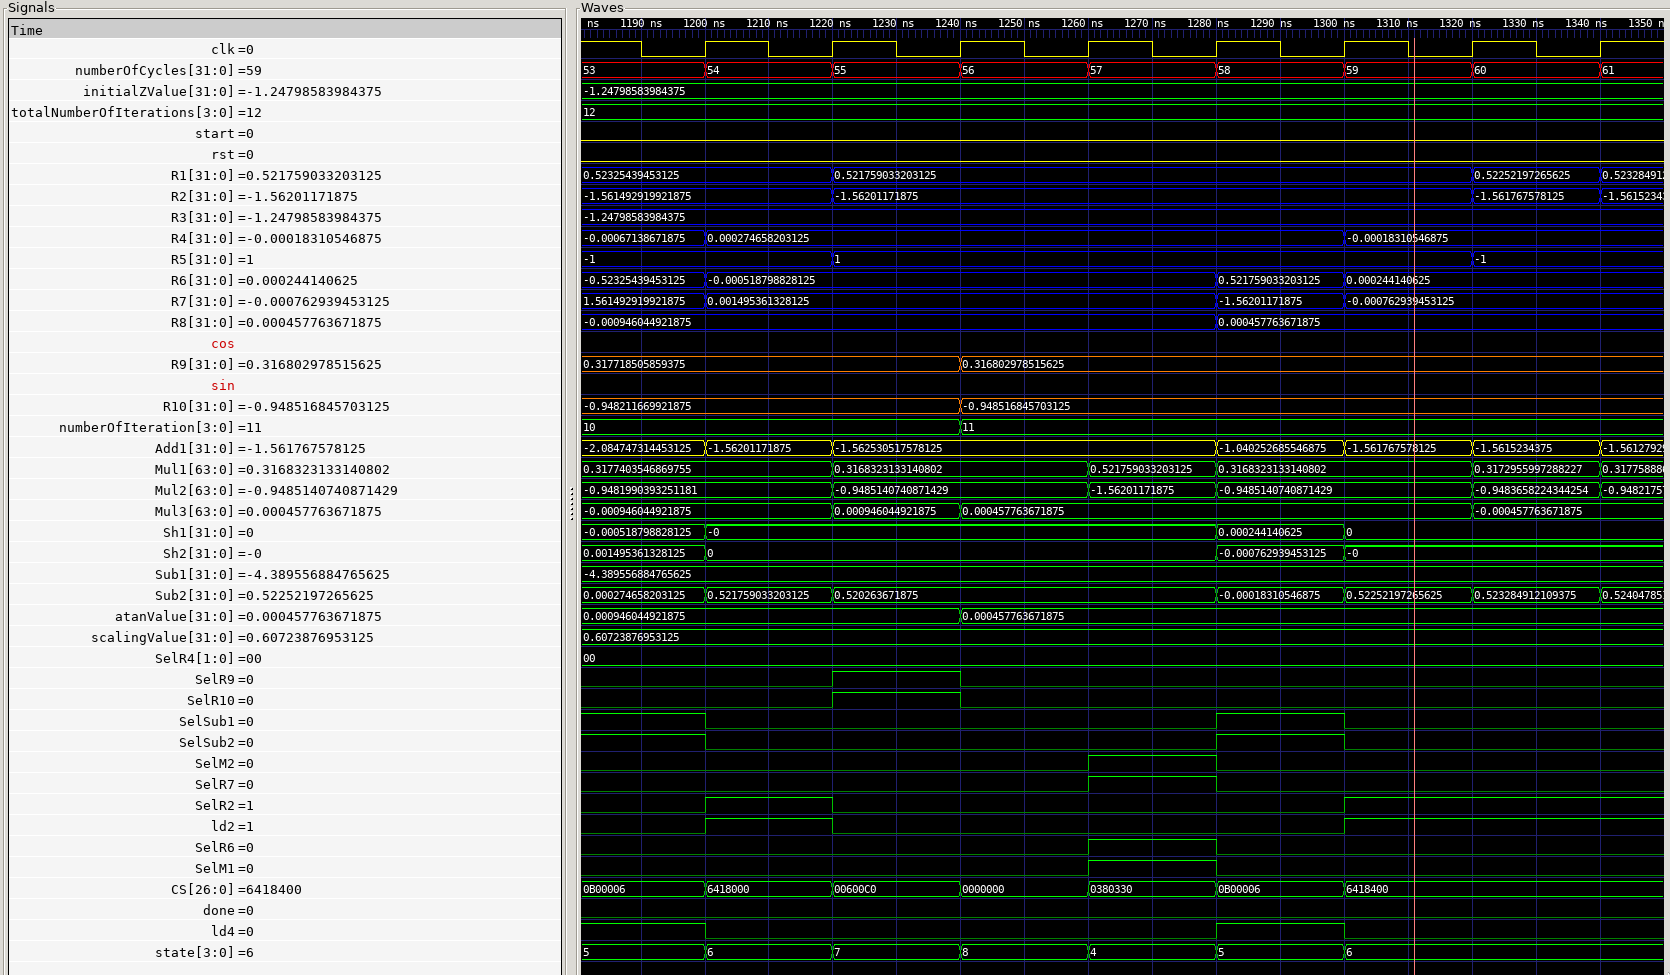
\includegraphics[width=1\textwidth]{src/png/cordic-verilog-end-of-the-simulation.png}
            \caption{The detail of the last iteration of the Verilog simulation of \gls{abbreviation:cordic} algorithm for determining the sine and cosine values of angle $\theta = -1.2479$ rad. The result is passed to the registers R9 and R10.}
            \label{fig:cordic-verilog-end-of-the-simulation}
        \end{figure}

        \begin{figure}[htbp!]
            \centering
            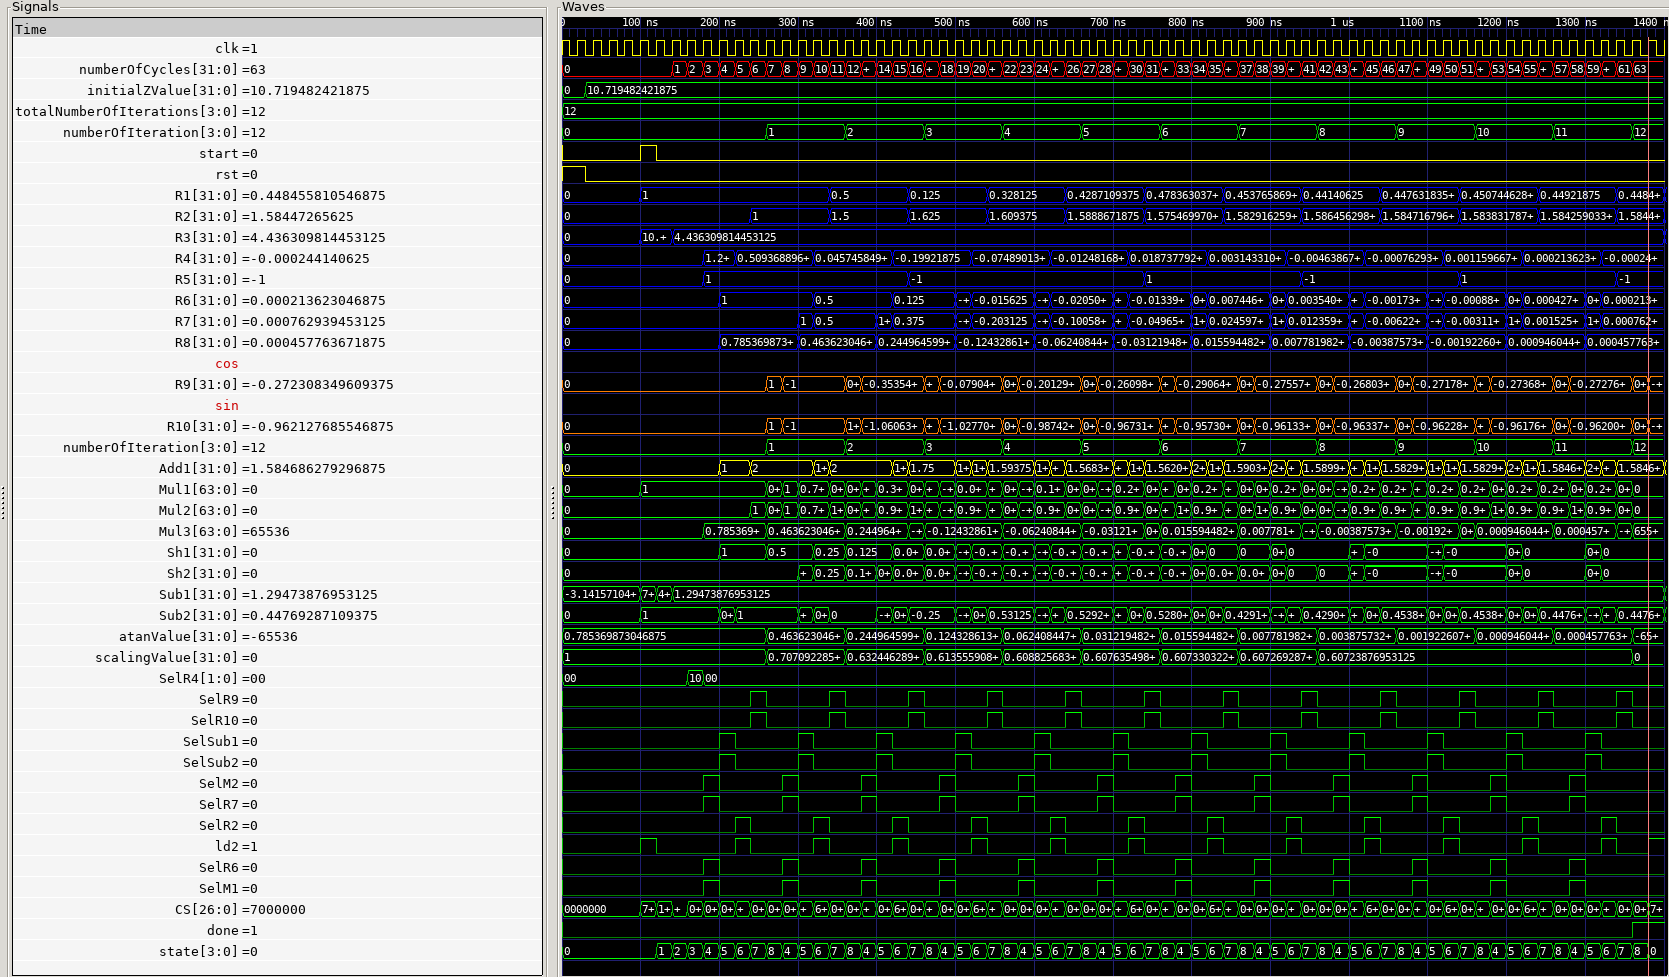
\includegraphics[width=1\textwidth]{src/png/cordic-verilog-whole-sim-10_719.png}
            \caption{The whole Verilog simulation of \gls{abbreviation:cordic} algorithm for determining the sine and cosine values of angle $\theta = 10.7195129$ rad. The value of sinus and cosinus based on the current iteration is also calculated in this algorithm approach. The result is passed to the registers R9 and R10.}
            \label{fig:cordic-verilog-whole-sim-10_719}
        \end{figure}

        \begin{figure}[htbp!]
            \centering
            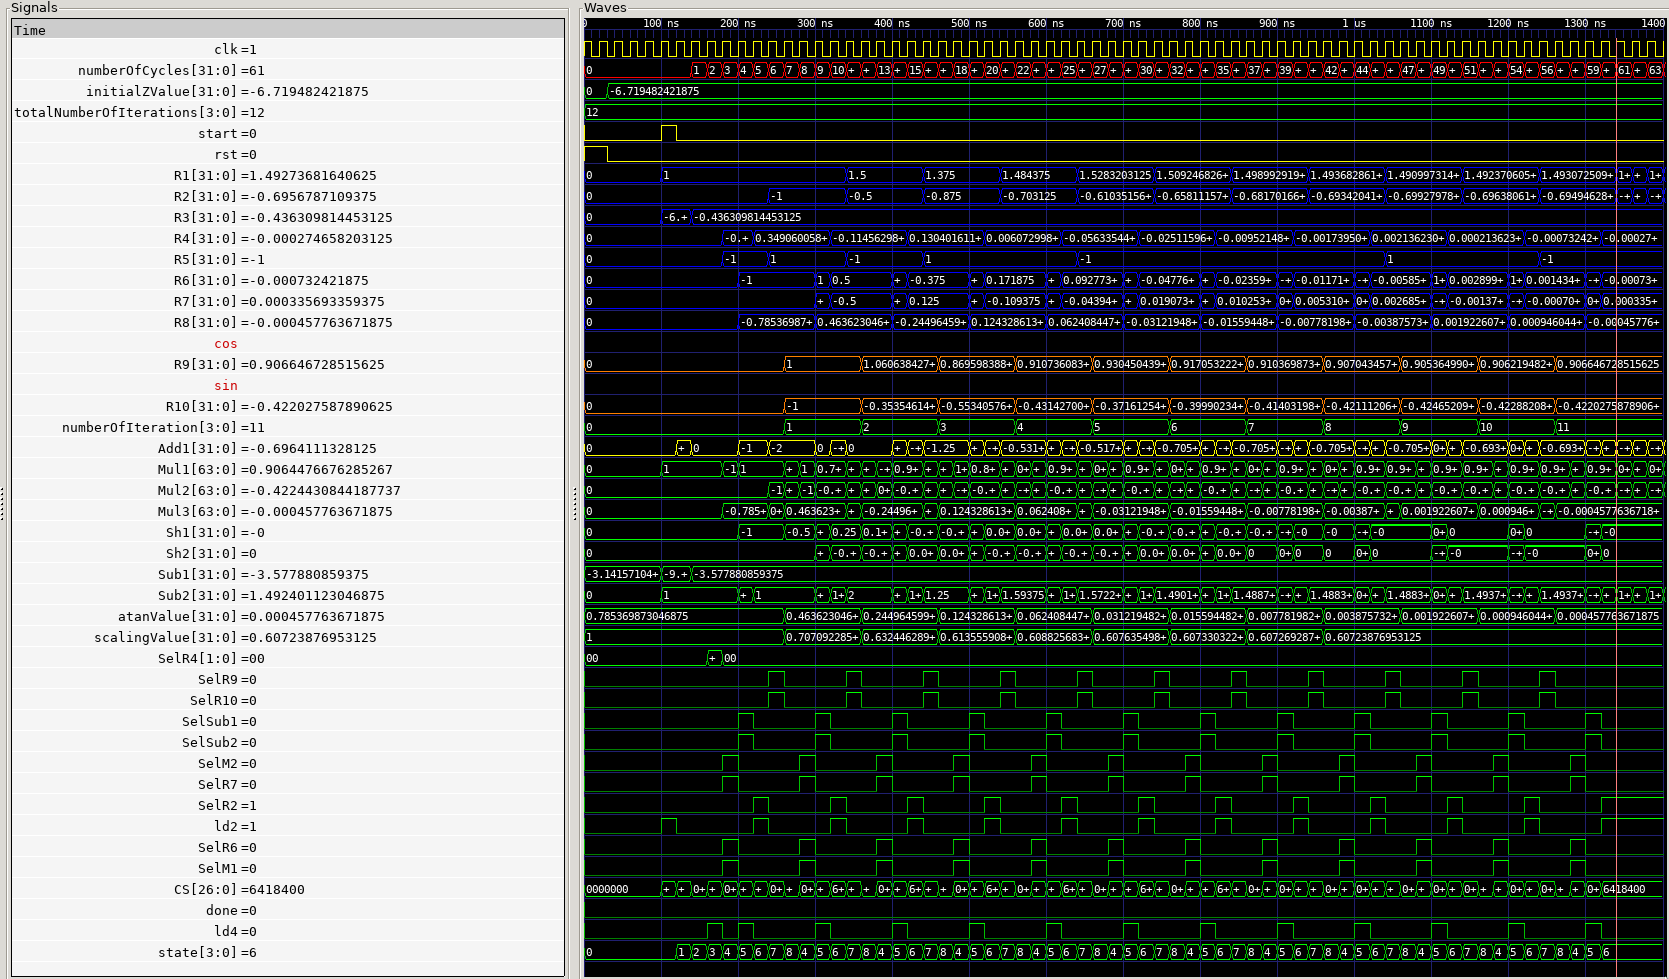
\includegraphics[width=1\textwidth]{src/png/cordic-verilog-whole-sim_minus_6_7195129.png}
            \caption{The whole Verilog simulation of \gls{abbreviation:cordic} algorithm for determining the sine and cosine values of angle $\theta = - 6.7195129$ rad. The value of sinus and cosinus based on the current iteration is also calculated in this algorithm approach. The result is passed to the registers R9 and R10.}
            \label{fig:cordic-verilog-whole-sim_minus_6_7195129}
        \end{figure}

\section{Simple set of nonlinear equations solved by a Newton-Raphson algorithm using custom circuit implementation}\label{sec:simple-set-of-nonlinear-equations-solved-by-a-newton-raphson-algorithm-using-custom-circuit-implementation}
    Most of the modules presented in the preceding sections can be utilized as submodules to solve the system of nonlinear equations. Because this work aims to solve the transcendetal equations for Selective Harmonic Elimination (\gls{abbreviation:she}), the most effective approach is to initially solve a simpler set of equations to determine, the difficulty and viability of the \gls{abbreviation:nr}.
    \subsection{Theory}
        The objective of the \gls{abbreviation:nr} algorithm is to solve the set of nonlienar equations


        \begin{equation}
            \text{F}_1 (x_1, x_2) = x_1^3 - x_2 - 1, 
        \end{equation}

        \begin{equation}
            \text{F}_2 (x_1, x_2) = x_1 - 2 x_2 - 2, 
        \end{equation}

        where one possible set of solutions $x_1$ and $x_2$ yields

        \begin{equation}
            \text{F}_1 = 0, 
        \end{equation}
        \begin{equation}
            \text{F}_2 = 0.
        \end{equation}

        \par
        The algorithm could have been implemented in a custom \gls{abbreviation:cpu} with reduced instruction set. However, due to apparent reasons such as speed and complexity associated with developing own processor, chosen approach involved creating an application specific circuit design.\par
        In order to integrate the algorithm into the custom design, the general \gls{abbreviation:nr} algorithm approach had to be simplified to the its most fundamental implementation. Every component that could be precalculated was set as a static value during the design phase.\par
        To check if the implementation and algorithm was well designed, the solution by \textit{Solve} function and a customized \gls{abbreviation:nr} was made in Wolfram Mathematica.\par
        Before initiating the algorithm, the starting values of $x_1^0$ and $x_2^0$ were set as inputs to the module. Based on that input the function values at selected starting points were calculated.\par
        As a next step, the so called defect could be calculated using the newly found values of $\text{F}_1 (x_1^0, x_2^0)$ and $\text{F}_2 (x_1^0, x_2^0)$

        \begin{equation}
            \Delta \textbf{F}^i =
            \begin{pmatrix}
                \Delta \text{F}_1^i\\
                \Delta \text{F}_2^i\\
            \end{pmatrix}
            =
            \begin{pmatrix}
                \text{F}_1^i - \text{F}_1^{\text{known solution}}\\
                \text{F}_2^i - \text{F}_2^{\text{known solution}}
            \end{pmatrix},
        \end{equation}
        where the superscript $i$ is the number of iteration for which the defect is calculated. When the algorithm starts, the $i = 0$. So for example the input value for $\text{F}_1^0$ is $x_1^0$ and $x_2^0$.\par
        Next, the Jacobian matrix \textbf{J} from vector of functions $\textbf(F)(x_1, x_2) = (\text{F}_1, \text{F}_2)$ is calculated as follows.

    \begin{equation}
        \textbf{J}^i = 
        \begin{pmatrix}
            \frac{\dd \text{F}_1}{\dd x_1^i} & \frac{\dd \text{F}_1}{\dd x_2^i}\\
            \frac{\dd \text{F}_2}{\dd x_1^i} & \frac{\dd \text{F}_2}{\dd x_2^i}
        \end{pmatrix}
        =
        \begin{pmatrix}
            3 (x_1^i)^2 & -1\\
            1 & -2
        \end{pmatrix}.
    \end{equation}

    As for the general \gls{abbreviation:nr} algorithm, the inverted value Jacobian matrix needs to be calculated. The problem is, that when using general mathematical software, such as Wolfram Mathematica, the calculation of the inversion is as easy as using function of inversion. When designing the circuit, the approach of manual calculation of inversion must be used. In this paper, the calculation is made possible by calculating the determinant of the Jacobian Matrix, its reciprocal value, its adjugate matrix and multiplication of the adjugate matrix elements by the calculated determinant reciprocal value.\par
    Because the size of the Jacobian matrix is 2x2 the determinant may be easily calculated using the Sarrus Rule. When the matrix is more complicated, the expansion method may be utilized.

    \begin{equation}
        \text{det}(\textbf{J}) = 3 (x_1^i)^2 (-2) - (-1) = 3 (x_1^i)^2 (-2) + 1.
    \end{equation}

    The reciprocal value of the determinant is then calculated by the Division Unit, created for calculating division of arbitrary real numbers. This Division Unit is presented in the section \hyperref[sec:calculating-the-division-of-fixed-point-numbers]{\textit{Calculating the division of fixed point numbers}}.\par
The adjugate matrix is calculated as follows

    \begin{equation}
        \text{adj}(\textbf{J}) =
        \begin{pmatrix}
            \textbf{J}_{11} (-1)^{1+1} & \textbf{J}_{01} (-1)^{1+2}\\

            \textbf{J}_{10} (-1)^{1+2} & \textbf{J}_{00} (-1)^{2+2}\\
        \end{pmatrix} =
        \begin{pmatrix}
            -2 & -1\\
            1 & 3 (x_1^i)^2
        \end{pmatrix}.
    \end{equation}
\par
    After the calculation of the reciprocal value of the determinant of the Jacobi matrix and the adjugate matrix, the inverted Jacobi matrix may be finally calculated

    \begin{equation}
        \textbf{J}^{-1i} =
        \frac{1}{\text{det}(\textbf{J}^i)}
        \begin{pmatrix}
            \text{adj}(\textbf{J}^i_{00}) & \text{adj}(\textbf{J}^i_{01})\\
            \text{adj}(\textbf{J}^i_{10}) & \text{adj}(\textbf{J}^i_{10})
        \end{pmatrix}
        =
        \frac{1}{\text{det}(\textbf{J}^i)}
        \begin{pmatrix}
            -2 & -1\\
            1 & 3 (x_1^i)^2
        \end{pmatrix}.
    \end{equation}
\par
    Next the $(\Delta x_1^i, \Delta x_2^i)$ can be calculated using the inverted Jacobi matrix and the defect.

    \begin{equation}
        \begin{pmatrix}
            \Delta x_1^i \\
            \Delta x_2^i
        \end{pmatrix}
        =
        \begin{pmatrix}
            \textbf{J}_{00}^{-1,i} \;\Delta \text{F}_1^i + \textbf{J}_{01}^{-1,i} \;\Delta \text{F}_2^i\\ 
            \textbf{J}_{10}^{-1,i} \;\Delta \text{F}_1^i + \textbf{J}_{11}^{-1,i} \;\Delta \text{F}_2^i
        \end{pmatrix}.
    \end{equation}

    \par
    Now the next iteration value denoted as $i+1$ of $x_1$ and $x_2$ may be calculated

    \begin{equation}
        \begin{pmatrix}
            x_1^{i+1}\\
            x_2^{i+1}
        \end{pmatrix}
        =
        \begin{pmatrix}
            x_1^i + \Delta x_1^i\\
            x_2^i + \Delta x_2^i
        \end{pmatrix}.
    \end{equation}
\par
    With these new iteration values $x_1^{i+1}$ $x_2^{i+1}$ the loop for calculation starts again at the calculation of the new value $\text{F}_1^{i+1}$ $\text{F}_2^{i+1}$ which is presented at the start of this section.

    \subsection{IP Block Design}
        
        \fbar
        \subsubsection{Top module design}
            Figure \ref{fig:simple-nr-top-module} depicts the top module design of the circuit. The Control Unit sends control signals to the Data Path unit to make the calculations. As in all designs in this paper, the numbers are formatted in the \textit{Q32.15} fixed point format.
            \begin{figure}[htbp!]
                \centering
                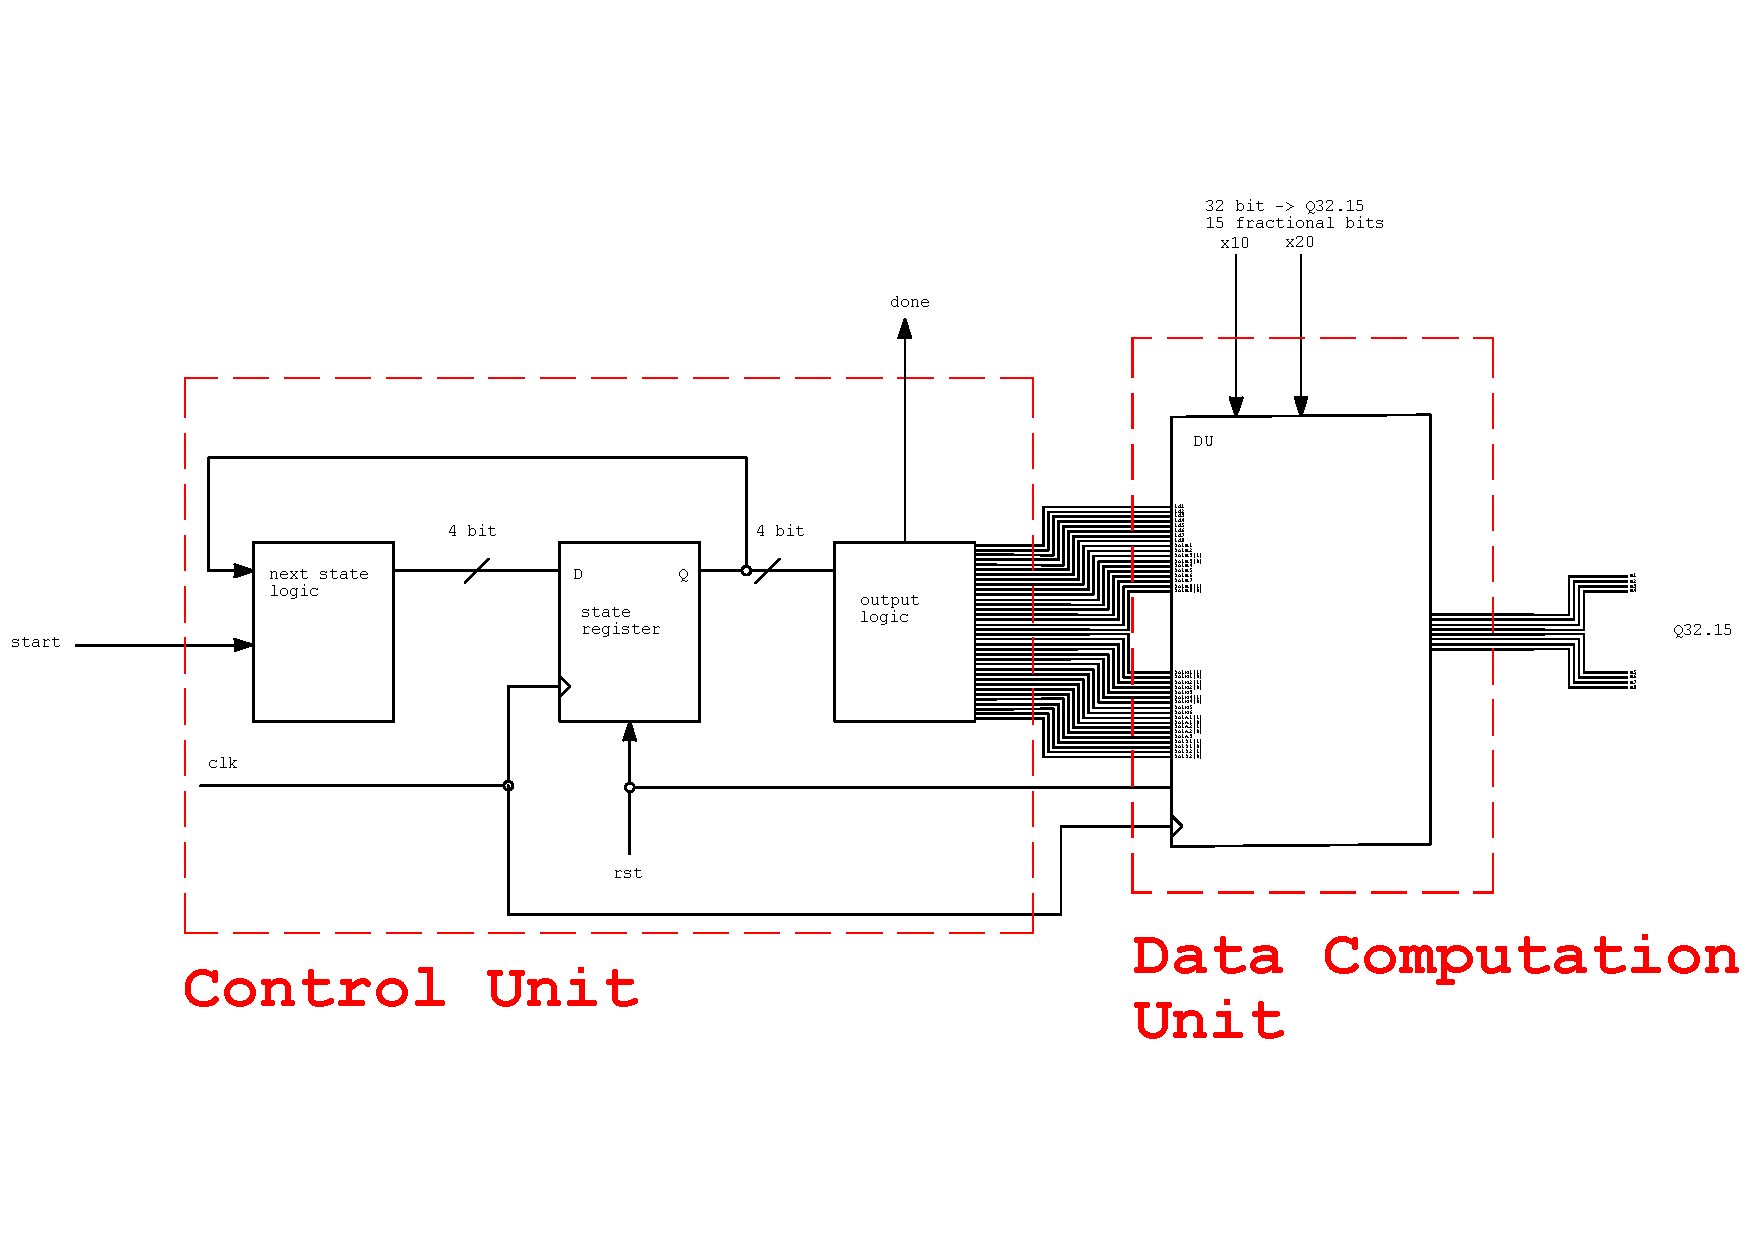
\includegraphics[width=1\textwidth]{src/pdf/simple-nr-top-module.pdf}
                \caption{Top module design for the simple Newton-Raphson (\gls{abbreviation:nr}) calculation module block design.}
                \label{fig:simple-nr-top-module}
            \end{figure}

        \fbar
        \subsubsection{Allocation and Timing}
            
            The algorithm structure for the Verilog implementation is depicted in the data flow diagram in the picture \ref{fig:simple-nr-allocation-timing}.
            \begin{figure}[htbp!]
                \centering
                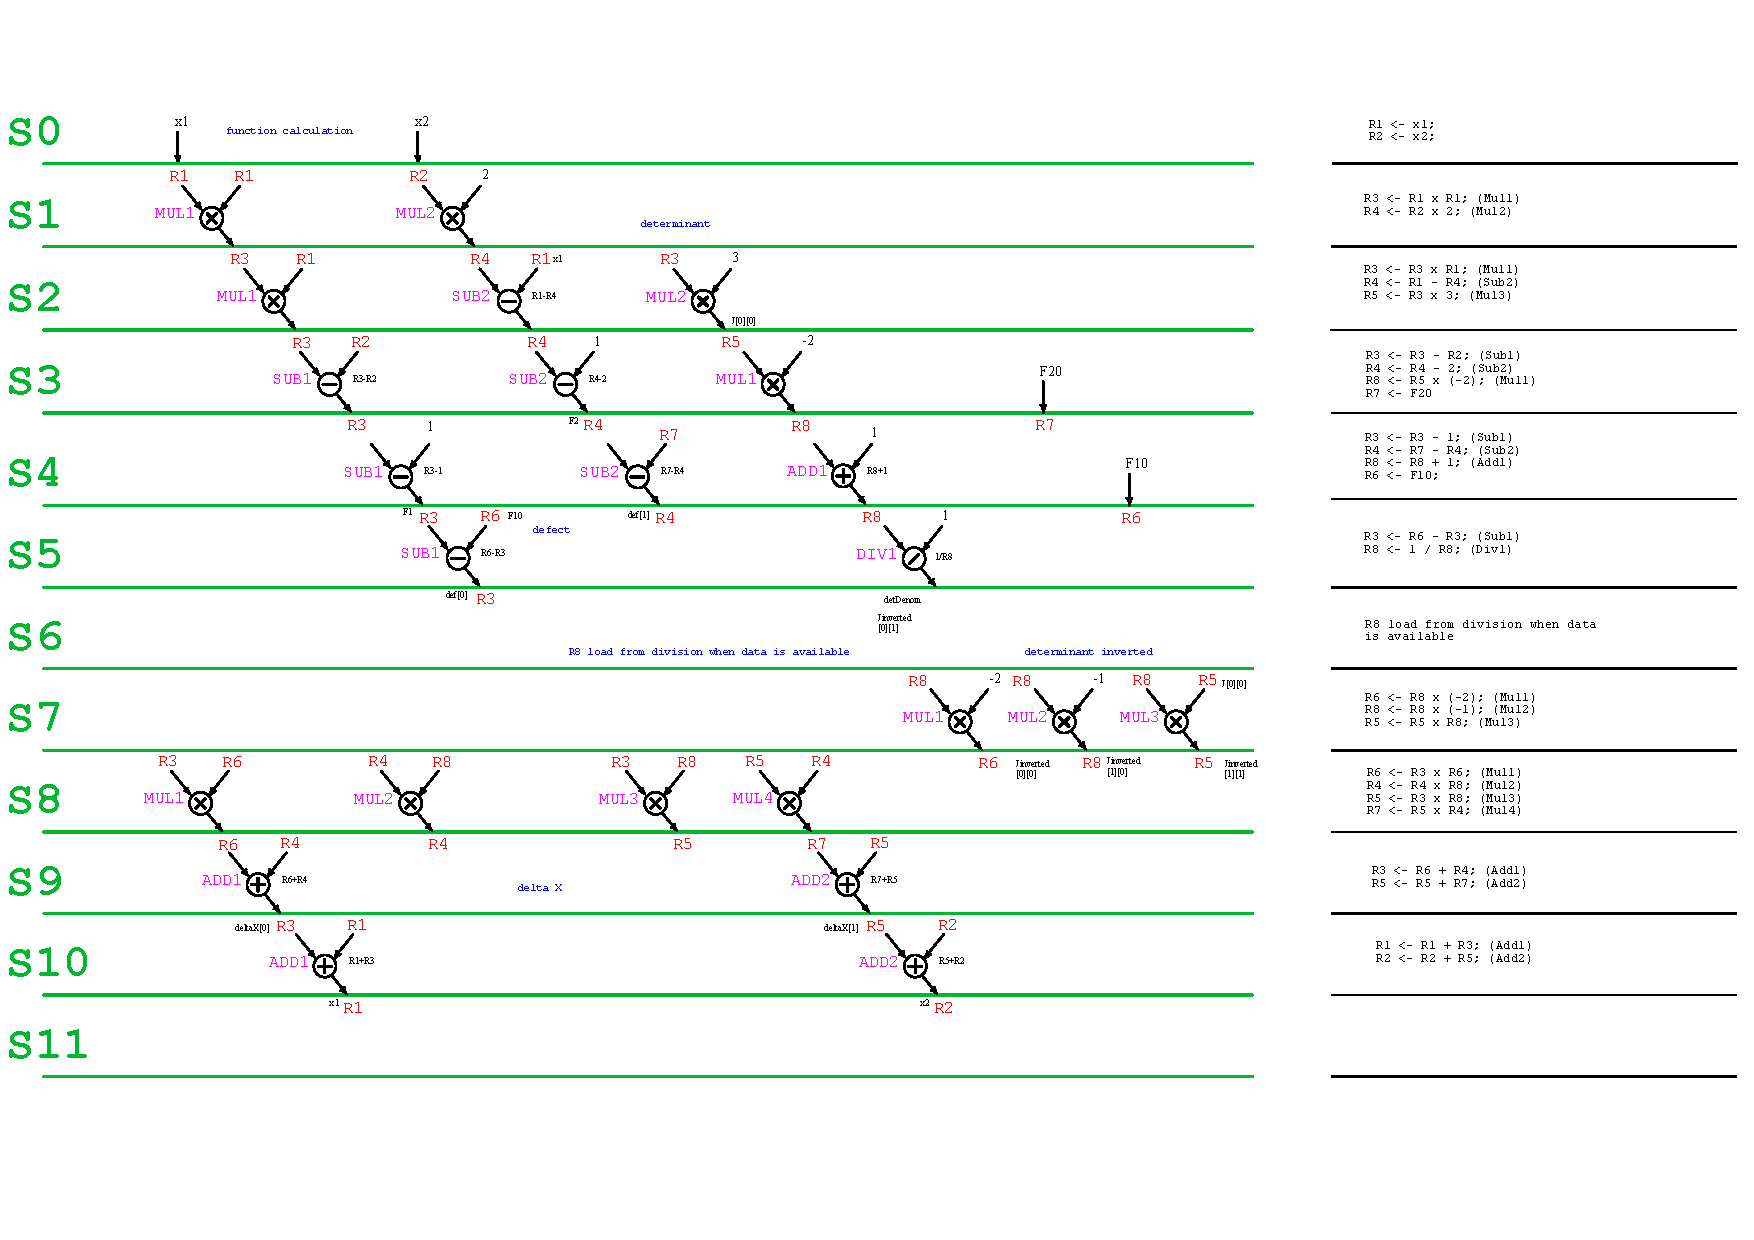
\includegraphics[width=1\textwidth]{src/pdf/simple-nr-allocation-timing.pdf}
                \caption{Allocation and timing diagram for the Data Path Unit part of the simple (\gls{abbreviation:nr}) module.}
                \label{fig:simple-nr-allocation-timing}
            \end{figure}

        \fbar
        \subsubsection{Data Path Unit}

            The Data path unit for this simple \gls{abbreviation:nr} algorithm consists of four multipliers, two adders, two subtractors and one divider. The divider is implemented using the Division Unit, presented in the section \hyperref[sec:calculating-the-division-of-fixed-point-numbers]{\textit{Calculating the division of fixed point numbers}}. Upon completion of the algorithm the results for $x_1$ and $x_2$ are saved in the R1 and R2, the state transitions to \textit{S11} and signal \textit{done} is set to 1. The results then can be driven to another module or unit for further usage.
            \begin{figure}[htbp!]
                \centering
                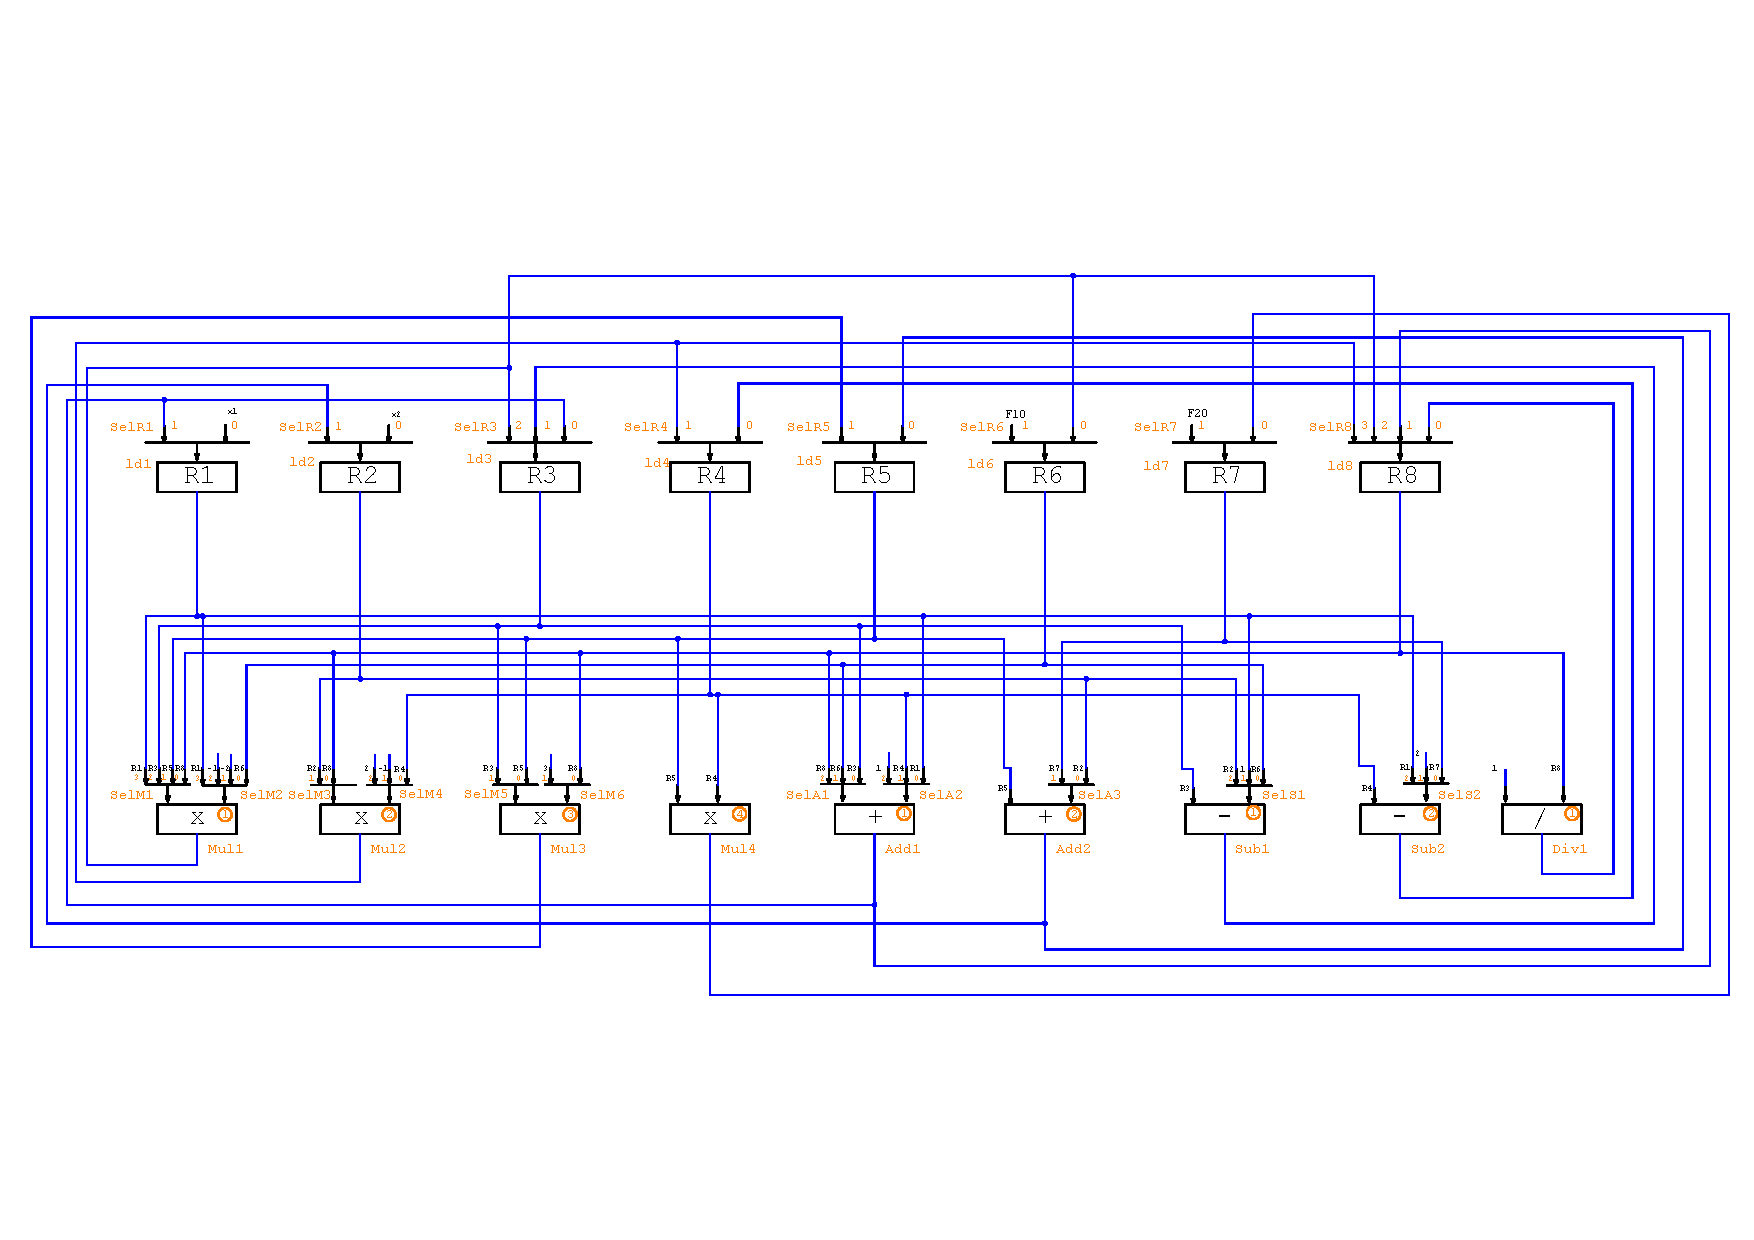
\includegraphics[width=1\textwidth]{src/pdf/simple-nr-rtl.pdf}
                \caption{Register Transfer Level (\gls{abbreviation:rtl}) scheme of the Data Path Unit part of the simple Newton-Raphson (\gls{abbreviation:nr}) calculation \gls{abbreviation:ip}.}
                \label{fig:simple-nr-rtl}
                \end{figure}

        \fbar
        \subsubsection{Control Unit}\label{subsubsec:simple-nr-control-unit}

            The Table \ref{tab:control-signal-simple-nr} shows encoding of a control signal for the Data Path unit.\par
            The \gls{abbreviation:nr} algorithm iteration transitions from the state \textit{S10} to state \textit{S1} when the iteration count is lower than the predetermined total number of iterations, value which is set in the Control Unit during the design phase. In this particular implementation, the total number of iterations is set to 5. It is worth noting that sometimes the termination of the \gls{abbreviation:nr} algorithm is determined by the value of a defect. However, in this implementation the defect-check is not implemented.\par
            Implementation of a defect-controlled algorithm would be straightforward. The values from registers holding the defect values, R3 and R4, would be connected to the control unit in the steps \textit{S4} and \textit{S5} respectively, and a comparison with the reference defect value would be executed. If the defect value was smaller than the reference value, the algorithm would transition to the state \textit{S11} and therefore the calculation would end. Conversely, ff the defect was larger than the reference value, the next state would be \textit{S6} and the iteratioun would proceeed normally, transitioning from state \textit{S10} to \textit{S1}.

            \subfile{src/tex/simple-nr-control-unit-table.tex}

    \fbar
    \subsection{Simulation results}
        The test bench for simulation was made using Cocotb \cite{cocotb} with the Verilator \cite{verilator} as a simulator. The results of the calculation may be seen in the registers R1 and R2. The results are $x_1 = - 0.707489$ and $x_2 = - 1.353759$.\par
        The clock signal frequency in simulation was set to 20 MHz.
            \begin{figure}[htbp!]
                \centering
                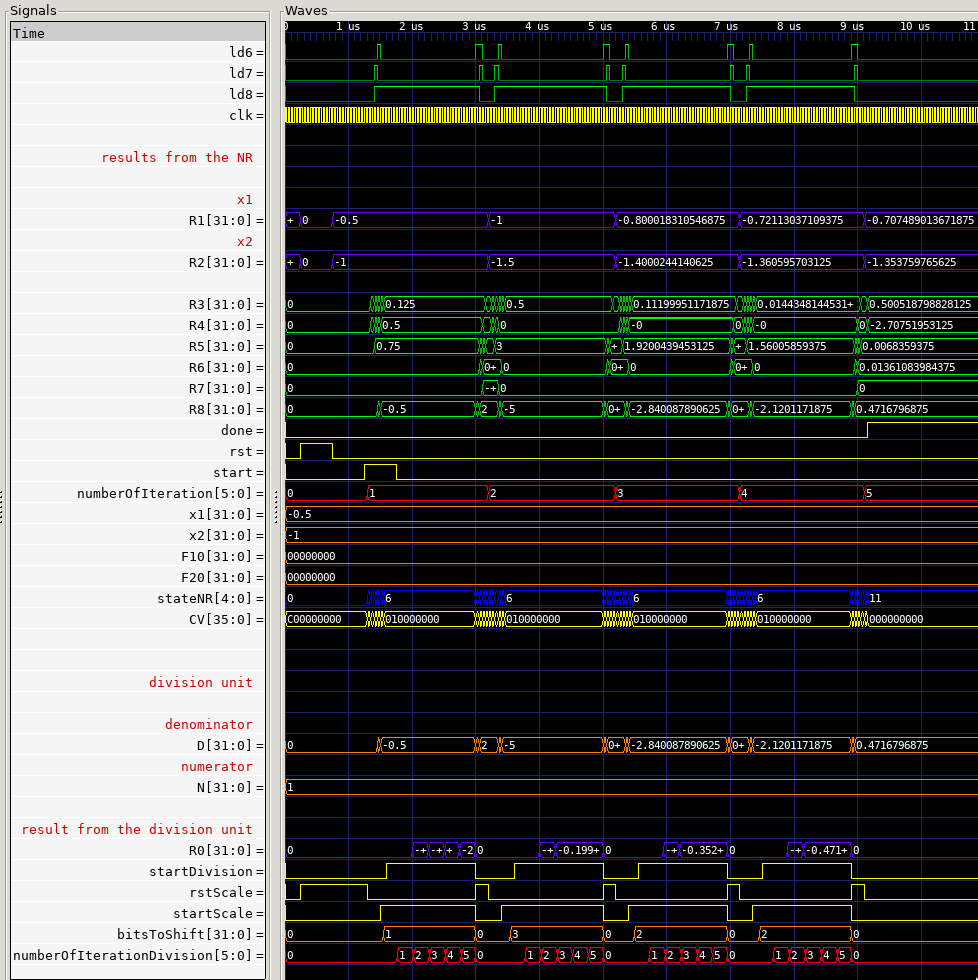
\includegraphics[width=1\textwidth]{src/png/simple-nr-sim.png}
                \caption{The whole Verilog simulation of a simple Newton-Raphson (\gls{abbreviation:nr}) algorithm. The result may be seen in registers R1 and R2 after the fifth iteration of the algorithm.}
                \label{fig:simple-nr-sim}
            \end{figure}



\section{Selective Harmonic Elimination}\label{sec:selective-harmonic-elimination}
    \subsection{Theory}\label{subsec:she-theory}
    The original theory for Selective Harmonic Elimination was initially developed in \cite{patel-Generalized-Techniques-of-Harmonic-Elimination-and-Voltage-Control-in-Thyristor-Inverters:-Part-I--Harmonic-Elimination, patel-Generalized-Techniques-of-Harmonic-Elimination-and-Voltage-Control-in-Thyristor-Inverters:-Part-II-----Voltage-Control-Techniques} and later adopted by numerous researchers for various voltage inverter topologies. Currently, the strategy is primarly employed in traction applications after start up state ends and the reference voltage for the drive is high enough so the six step output voltage is utilized. However, the general six step output signal produces high-order harmonics. When the motor is powered by these high-order voltage harmonics, the current with high-order harmonics (excluding triplen harmonics, considering the symmetric 3 phase motor) is observed. These current harmonics result in undesirable current ripple, torque ripple and losses \cite{mullner-Modelling-and-precalculation-of-additional-losses-of-inverter-fed-asynchronous-induction-machines-for-traction-applications}, thereby decreasing the efficiency of the drive.\par
    To control the output voltage and reduce unwanted harmonics, the Selective Harmonic Elimination (\gls{abbreviation:she}) technique can be employed. The elimination is based on generating the output voltage by switching components at certain phase angles, thereby generating waveform with a number of pulses, to corresponding the number of elliminated harmonics. The calculation which angles to use is based on the calculation of fourier coefficients. These equations, derived from the original principle, have been adapted for different types of converters, including multilevel, H-bridge converters or generic Voltage Source Inverters (\gls{abbreviation:vsi}). In this paper, the regular two level \gls{abbreviation:vsi} is considered.\par
    The considered inverter phase voltage six-step waveform is depicted in Figure \ref{fig:SixStepPlotWaveform}, while the harmonic analysis of the generic waveform is depicted in Figure \ref{fig:SixStepPlotHarmonics}.  It's worth noting that in a three-phase symmetrical system, the triplen harmonics are also eliminated.
            \begin{figure}[htbp!]
                \centering
                \begin{subfigure}[t]{0.45\textwidth}
                    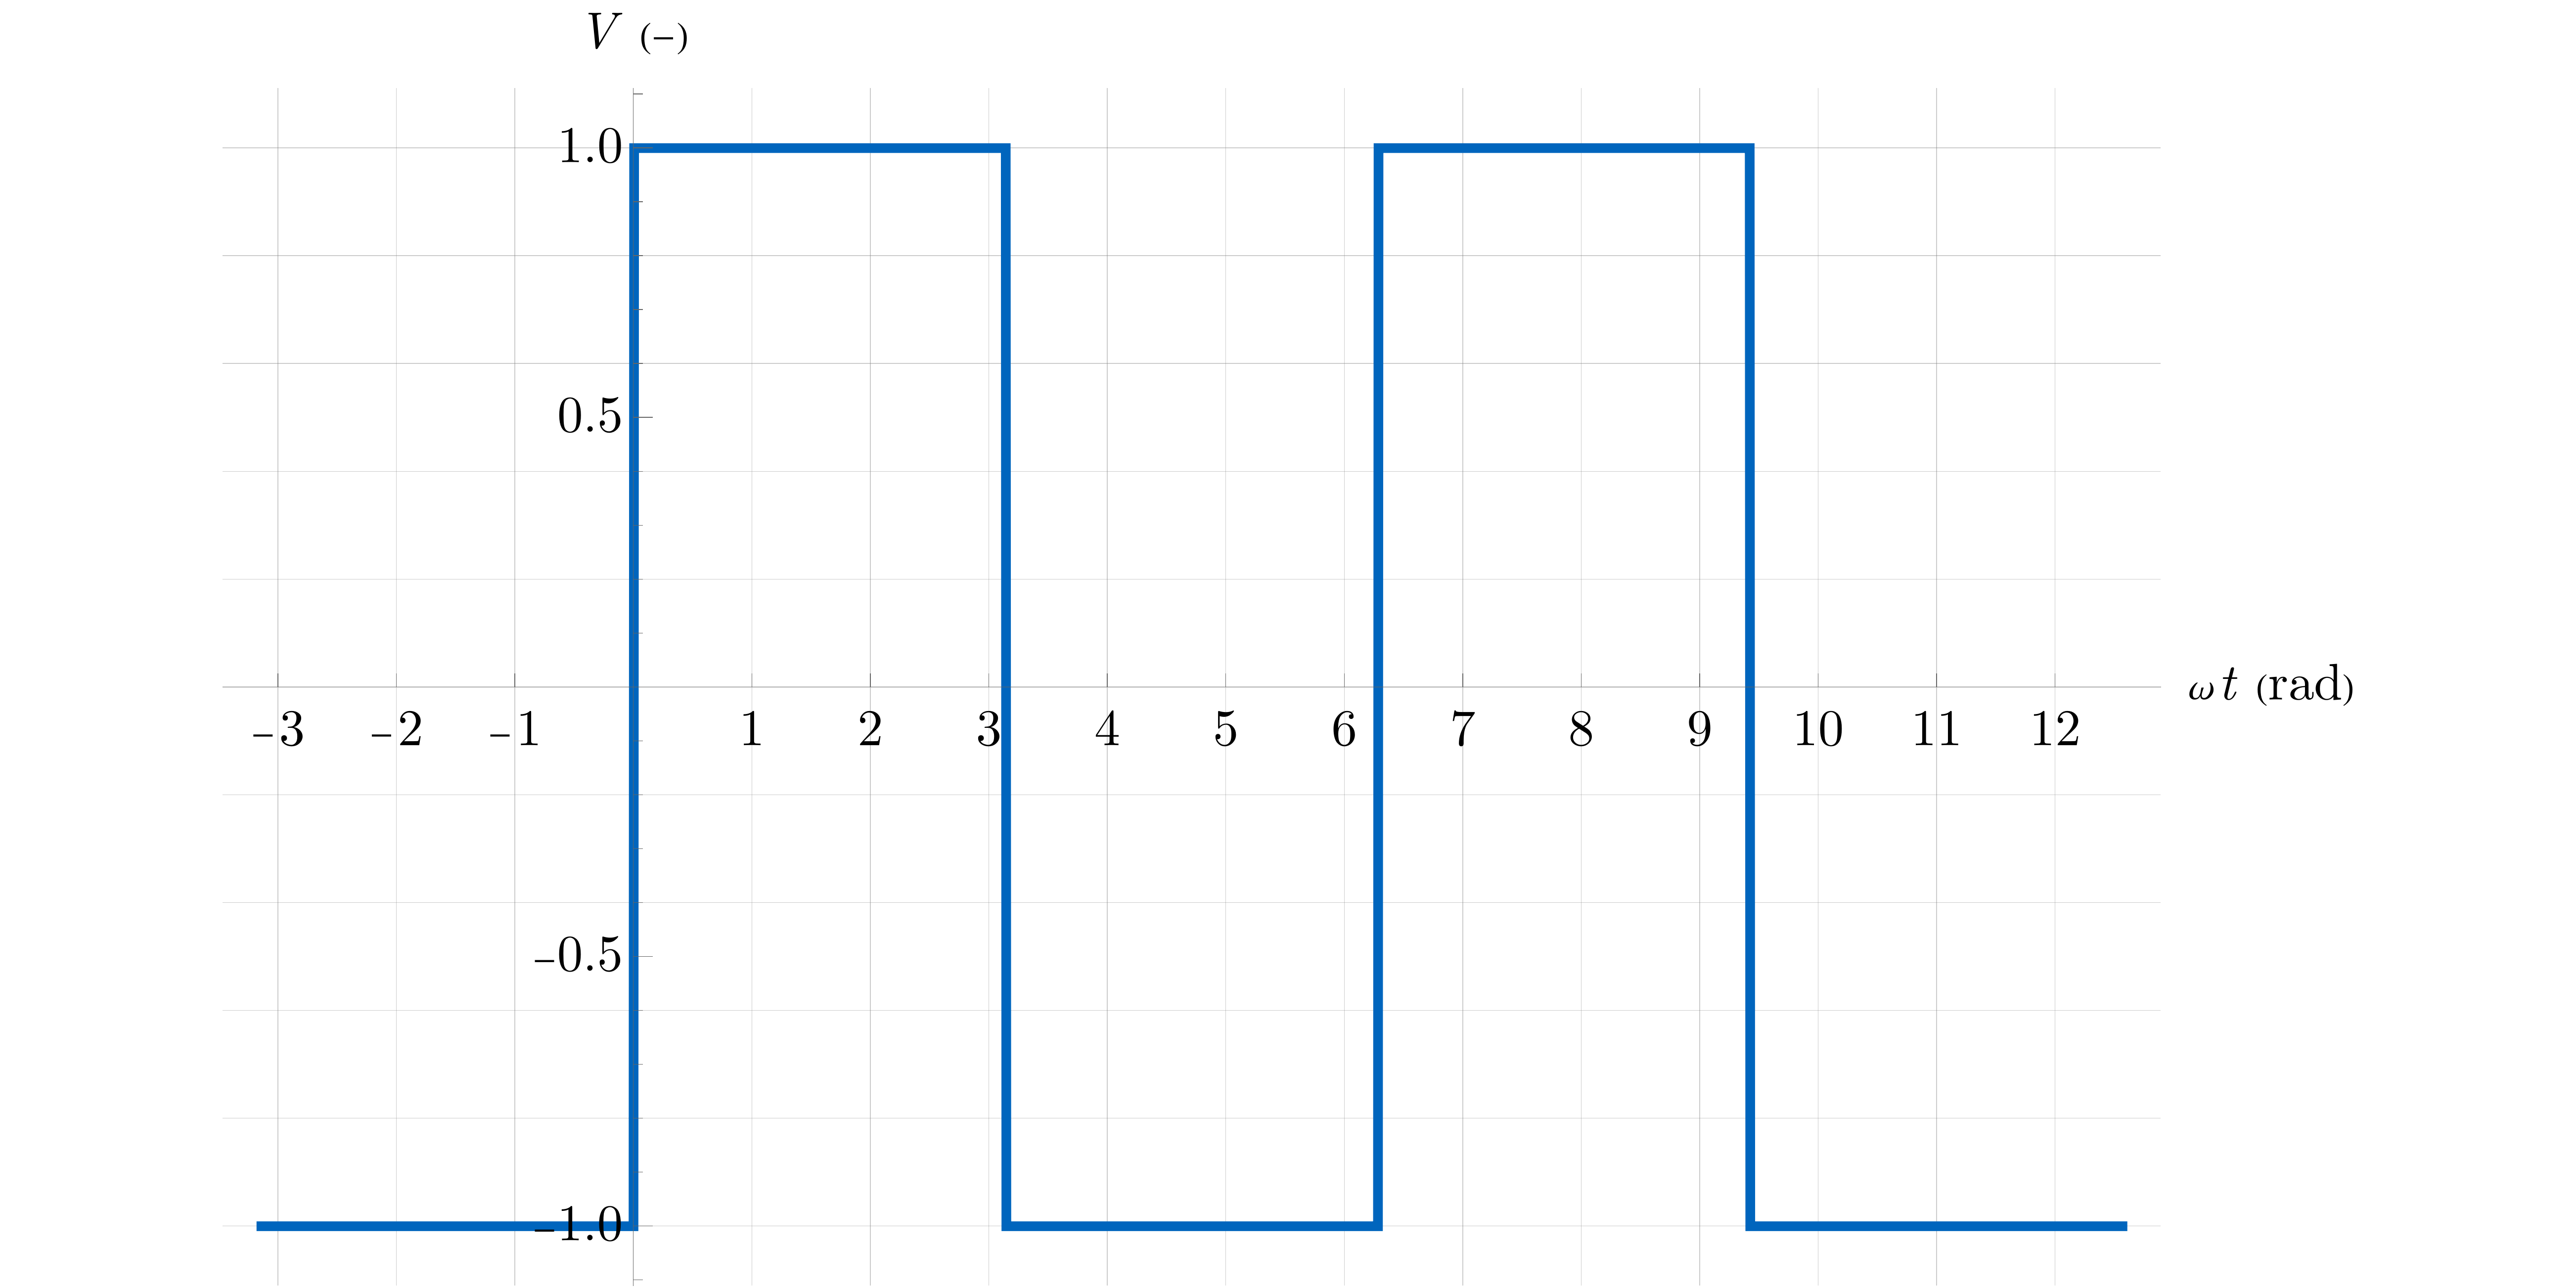
\includegraphics[width=1\textwidth]{src/png/SixStepPlotWaveform.png}
                    \caption{Generic Six-Step Waveform output of a two level Voltage Source Inverter. The Voltage value is normalized to a \gls{abbreviation:dc} link voltage.}
                    \label{fig:SixStepPlotWaveform}
                \end{subfigure}
                \hspace{0.05\textwidth}
                \begin{subfigure}[t]{0.45\textwidth}
                    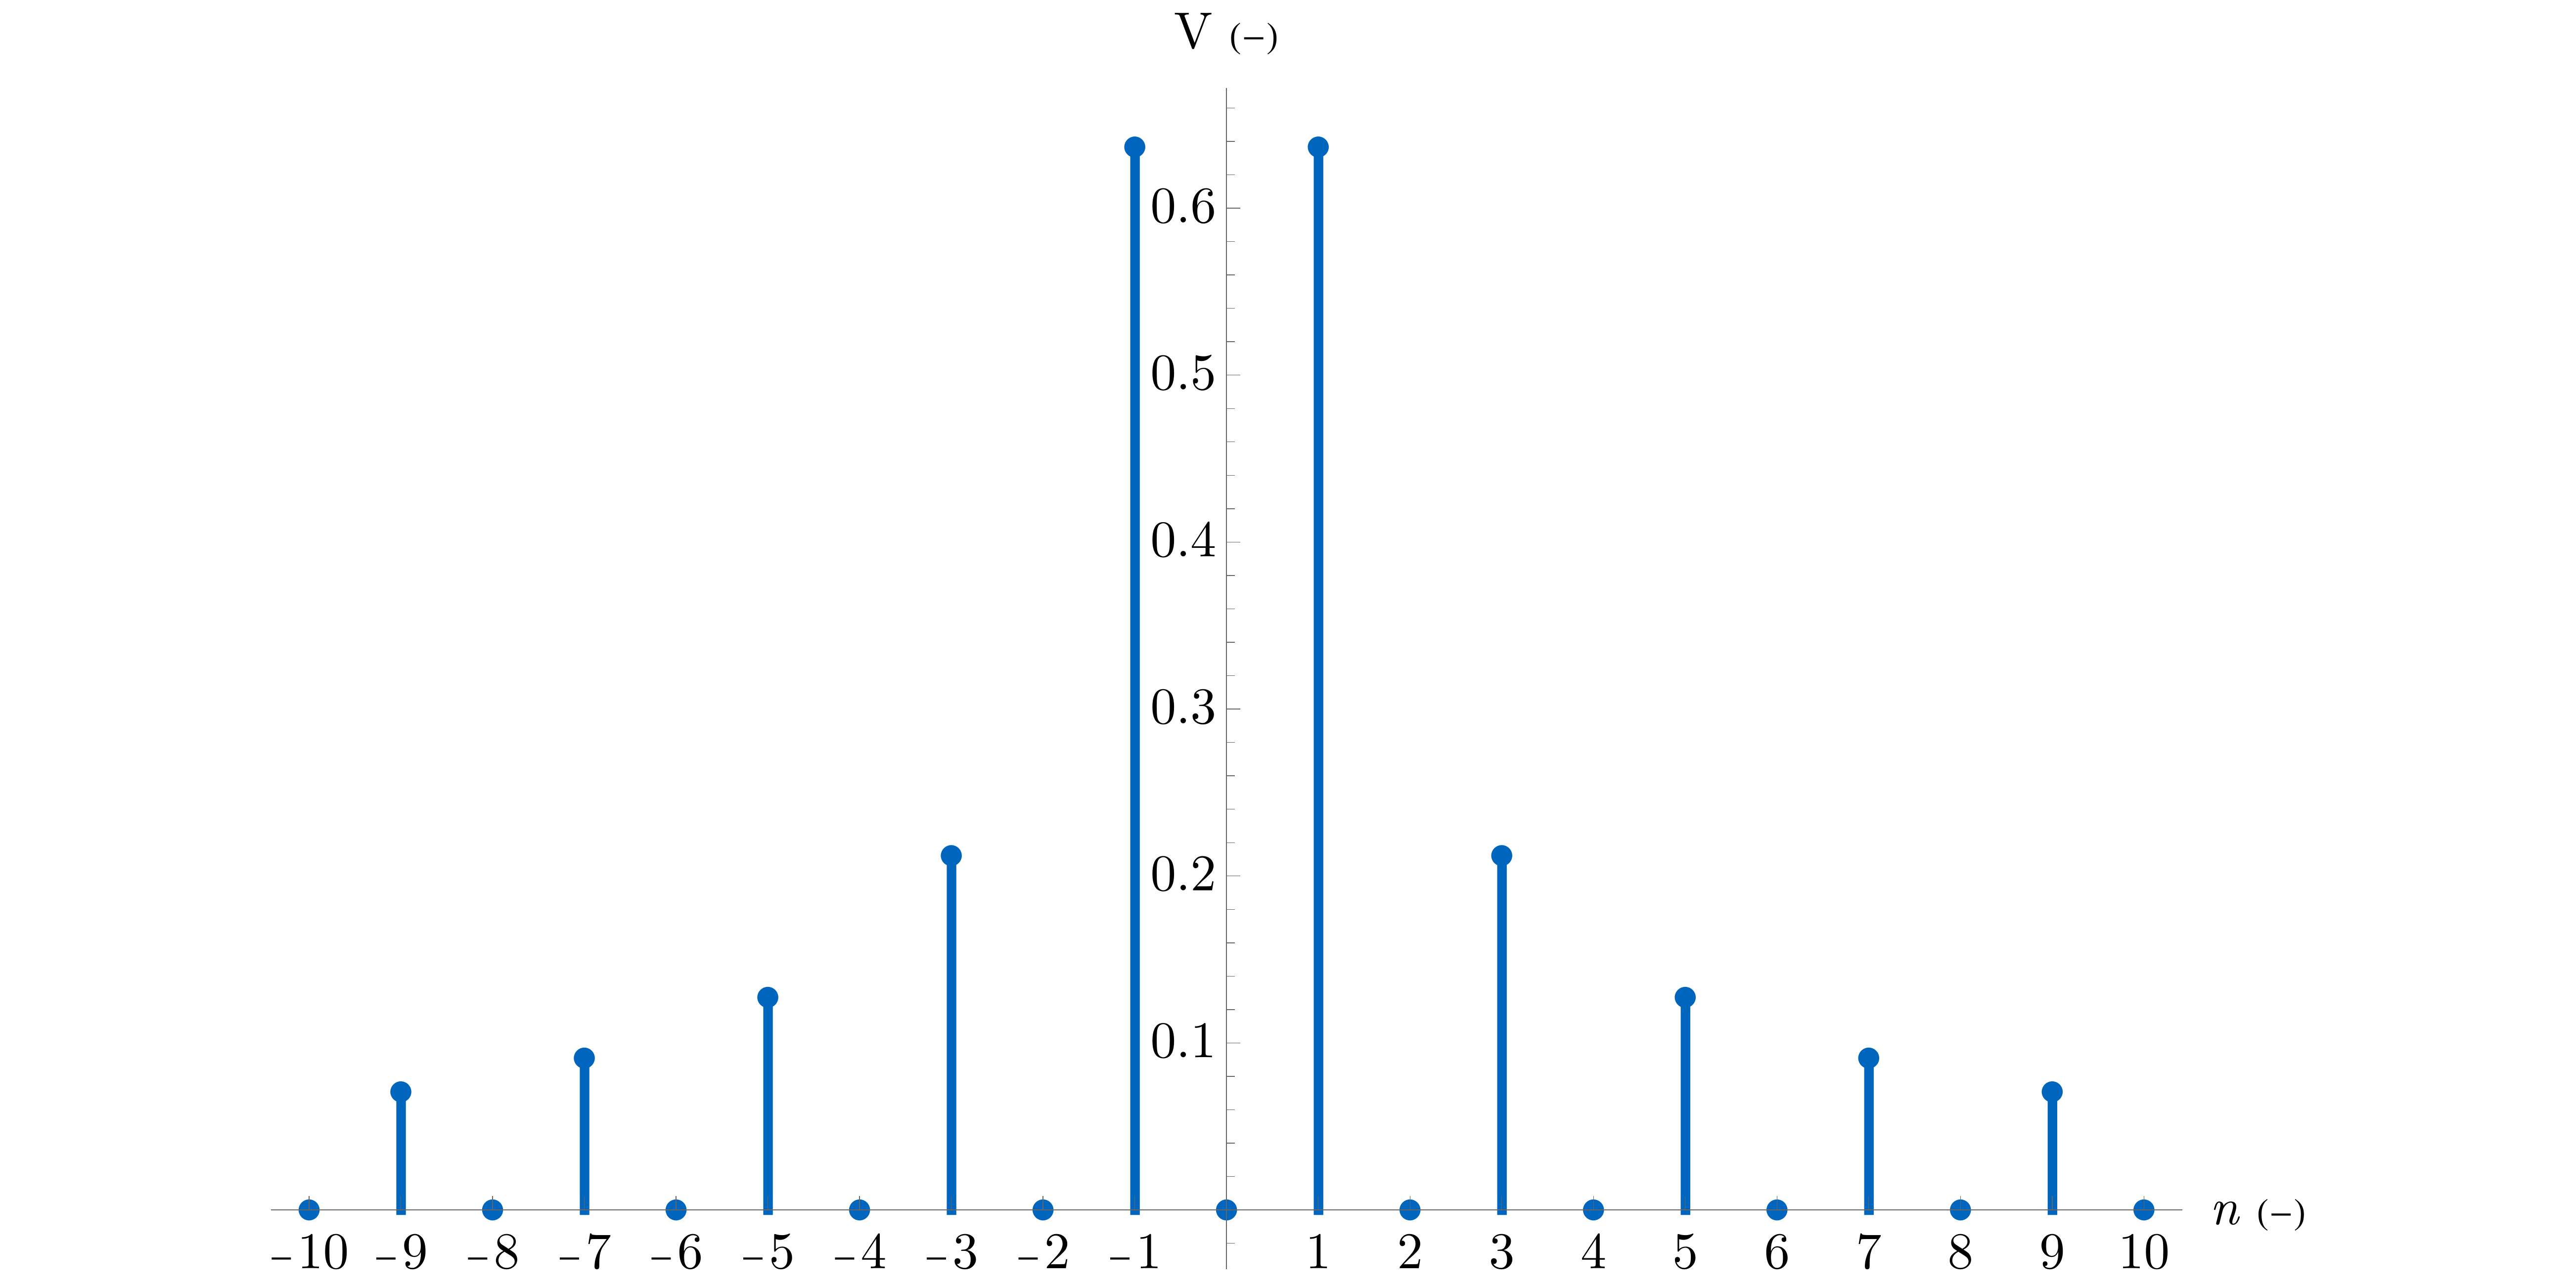
\includegraphics[width=1\textwidth]{src/png/SixStepPlotHarmonics.png}
                    \caption{Generic Six-Step Waveform harmonics analysis. The Voltage value is normalized to a DC link voltage.}
                    \label{fig:SixStepPlotHarmonics}
                \end{subfigure}
                \caption{}
            \end{figure}
            \FloatBarrier
            As previously mentioned, the \gls{abbreviation:she} method is based on a Fourier coefficient analysis. When the odd quarter-wave symmetry of the waveform is assumend, the $a_n$ Fourier coefficient is zero (as mentioned in the Equation \ref{eq:she-first-fourier-coefficient-zero}), whereas the $b_n$ coefficient may be written as Equation \ref{eq:she-second-fourier-coefficient}.

            \begin{equation}
                a_n = 0,
                \label{eq:she-first-fourier-coefficient-zero}
            \end{equation}

            \begin{equation}
                b_n = \frac{2}{T} \int_{0}^{T} x(n\omega t)\sin(\omega t) \dd \omega t,
                \label{eq:she-second-fourier-coefficient}
            \end{equation}
            where the $T$ is signal periode, $x(\omega t)$ description of the \gls{abbreviation:vsi} output voltage waveform and $n$ is the order of the harmonics.

            When assuming quarter-wave symmetry the Equation \ref{eq:she-second-fourier-coefficient} may be rewritten as

            \begin{equation}
                b_n = \frac{8}{T} \int_{0}^{T/4} x(\omega t) \sin (n\omega t) \dd \omega t = \frac{8}{2 \pi} \int_{0}^{2 \pi/4} x(\omega t) \sin (n\omega t) \dd \omega t = \frac{4}{\pi} \int_{0}^{\frac{\pi}{2}} x(\omega t) \sin (n\omega t) \dd \omega t.
            \end{equation}

            The function $x(\omega t)$ represents the normalized output voltage pulse in relation to a \gls{abbreviation:dc} link voltage. The Equation \ref{eq:she-second-fourier-coefficient} can be reformulated by substituting $\omega t$ with the angle $\alpha$, which also characterizes the output waveform in terms of radians. The function $x(\alpha)$ yields $1$ when the output voltage pulse is positive and $-1$ when negative. The reformulated Equation \ref{eq:she-second-fourier-coefficient}, assuming quarter-wave symmetry, is then as follows:

            \begin{equation}
                b_n = \sum_{k=1}^{M} \frac{8}{T} \int_{\alpha_k}^{\alpha_{k+1}} x(\alpha) \sin(n\alpha) \dd \alpha.
            \end{equation}

           Here $M$ represents number of pulses in half period of the output signal. Assuming that the integral is calculated for angles where $x(\alpha_k)$ is either $1$ or $-1$, the function may be replaced by a constant. As a result, the integral calculation becomes straightforward.

           \begin{equation}
               \begin{gathered}
                    b_n = \frac{4}{\pi} \sum_{k=1}^{M} \frac{1}{n} \left[ - \cos(n\alpha) \right]_{\alpha_k}^{n\alpha_{k+1}}
                    = \frac{4}{\pi n} \sum_{k=1}^{M} \left[ \cos(n\alpha_k) - \cos(n\alpha_{k-1}) \right].
               \end{gathered}
               \label{eq:she-equation-integration}
           \end{equation}

           The Equation \ref{eq:she-equation-integration} can be further simplified by observing the results of the summation for $M = 2$.
            
            \begin{equation}
                \begin{gathered}
                    b_n = \frac{4}{\pi n} \sum_{k=1}^{2} \left[ \cos(n\alpha_k) - \cos(n\alpha_{k-1}) \right] = \frac{4}{\pi n} \left[ (\cos(n\alpha_1) - \cos(n\alpha_2)) + (\cos(n\alpha_2) - \cos(n\alpha_3)) \right]
                    =
                    \\
                    =
                    \frac{4}{\pi n} (\cos(n\alpha_1) - \cos(n\alpha_3)).
                \end{gathered}
            \end{equation}

            According to \cite{patel-Generalized-Techniques-of-Harmonic-Elimination-and-Voltage-Control-in-Thyristor-Inverters:-Part-I--Harmonic-Elimination} and the example calculation for $M = 2$, the further simplification of the Equation \ref{eq:she-equation-integration} is Equation \ref{eq:she-final-transcendetnal-equation}.

            \begin{equation}
                b_n = \frac{4}{\pi n} \sum_{k=1}^{M} (-1)^{k+1} \cos(n\alpha_k).
                \label{eq:she-final-transcendetnal-equation}
            \end{equation}

            It can be said, that the number of eliminated odd harmonics is $N = M-1$.\par

            To maintain clarity of this paper only the 5th harmonics is being eliminated by the designed unit. The set of equations required to eliminate this harmonic is as follows.

            \begin{equation}
                \begin{gathered}
                    V_1 = b_1 = \frac{4}{\pi} \left[ \cos(\alpha_1) - \cos(\alpha_2) \right],\\
                    V_5 = b_5 = \frac{4}{5 \pi} \left[ \cos(5 \alpha_1) - \cos(5 \alpha_2) \right].\\
                \end{gathered}
                \label{eq:she-set-of-base-equations}
            \end{equation}
            The amplitudes of the 1st and 5th harmonics are denoted as $V_1 = b_1$ and $V_5 = b_5$, respectively. For the elimination of the 5th harmonic, it is required that $b_5 = 0$. Consequentely, the set of Equations \ref{eq:she-set-of-base-equations} can be simplified as set of Equations \ref{eq:she-final-set-of-transcendental-equations}.

            \begin{equation}
                \begin{gathered}
                    \frac{4 V_1}{\pi} = \cos(\alpha_1) - \cos(\alpha_2),\\
                    0 = \cos(5 \alpha_1) - \cos(5 \alpha_2).\\
                \end{gathered}
                \label{eq:she-final-set-of-transcendental-equations}
            \end{equation}
            Solving the nonlinear Equations \ref{eq:she-final-set-of-transcendental-equations} is not straightforward. Barious methods can be employed for solving the problem, such as Genetic Algorithms \cite{taghizadeh-Harmonic-elimination-of-multilevel-inverters-using-particle-swarm-optimization, Ortiz-Espinoza-PWM-with-Selective-Harmonic-Elimination-Using-Optimization-Inspired-on-Earthquakes-for-AC-Electric-Drives, Abdelqawee_Naser-SELECTIVE-HARMONIC-ELIMINATION-PWM-VOLTAGE-SOURCE-INVERTER-BASED-ON-GENETIC-ALGORITHM} or algebraic methods \cite{wang-A-Comprehensive-Review-of-Solving-Selective-Harmonic-Elimination-Problem-with-Algebraic-Algorithms, Chiasson-A-Complete-Solution-to-the-Harmonic-Elimination-Problem}. One commonly used algebraic method is Newton-Raphson (\gls{abbreviation:nr}) algorithm \cite{Balow-A-Selective-Harmonic-Elimination-SHE-Technique-for-the-Multi-Leveled-Inverters}. In this paper, the solution is obtained solely using \gls{abbreviation:nr} algorithm. However, it's worth noting that the success of this method depends on setting the initial conditions correctly; otherwise, a solution may not be found. In contrast, Genetic Algorithms also require setting initial values, but they often use random numbers from predefined intervals.\par
            In real-time systems, the approach for solving the \gls{abbreviation:she} equations may often be to precalculate the required switching angles offline and the utilize the \gls{abbreviation:lut} in a microprocessor to determine which set of angles use for the set reference voltage. Nowadays the \gls{abbreviation:fpga}s are more frequently utilized to calculate the solution. The calculation can be highly paralelized and optimized, enabling the solution to be obtained in near real-time. In the following sections the prototype implementation in Python and final implementaion in Verilog are presented.

    \subsection{Simplification for Verilog and High level implementation}\label{subsec:simplification-for-verilog-and-high-level-implementation}
        When implementing the solution in computational software like Wolfram Mathematica, optimizing the algorithm is unnecessary. However, when implementing the algorithm to an \gls{abbreviation:fpga}, higher-level constructs are not automatically available, so the simplification is necessary. Before creating the Verilog design, it is suitable, for clarity and prototyping purposes, to implement the algorithm in Python. In this section, the simplified algorithm of a \gls{abbreviation:nr} aglorithm is presented.\par

        The set of equations for eliminating the 5th harmonics may be formulated as

        \begin{equation}
            \begin{gathered}
                \mathrm{F}_1^i = \cos(\alpha_1) - \cos(\alpha_2),\\
                \mathrm{F}_2^i = \cos(5\alpha_1) - \cos(5\alpha_2),\\
                \mathrm{where} \; \mathrm{F}_1^0 = m \; \frac{\pi}{4},\; \mathrm{F}_2^0 = 0.\\
            \end{gathered}
        \end{equation}
        Where $m = V_1/V_{\mathrm{DC}}$ is modulation index.\par
        Thus the Jacobian matrix is

        \begin{equation}
            \begin{gathered}
                \textbf{J}^i = 
                \begin{pmatrix}
                    - \sin(\alpha_1^i) & \sin(\alpha_2^i)\\
                    - 5 \sin(5\alpha_1^i) & 5 \sin(5\alpha_2^i)
                \end{pmatrix}.
            \end{gathered}
        \end{equation}
        Where $i$ is the index of the iteration of the algorithm. The inverted Jacobian matrix is needed for further calculations.

        \begin{equation}\label{eq:she-inverted-jacobian-matrix}
            \begin{gathered}
                \mathrm{J}^{-1,i} = 
                \begin{pmatrix}
                \frac{5 \sin(5\alpha_2^i)}{5 \sin(5\alpha_1^i) \sin(\alpha_2^i) - 5 \sin(\alpha_1^i)\sin(\alpha_2^i)} & - \frac{\sin(\alpha_2^i)}{5 \sin(5\alpha_1^i) \sin(\alpha_2^i) - 5 \sin(\alpha_1^i)\sin(\alpha_2^i)}\\
                    \frac{5\sin(\alpha_1^i)}{5 \sin(5\alpha_1^i) \sin(\alpha_2^i) - 5 \sin(\alpha_1^i)\sin(\alpha_2^i)} & - \frac{\sin(\alpha_1^i)}{5 \sin(5\alpha_1^i) \sin(\alpha_2^i) - 5 \sin(\alpha_1^i)\sin(\alpha_2^i)}
                \end{pmatrix}.
            \end{gathered}
        \end{equation}

        From the inverted Jacobian matrix in Equation \ref{eq:she-inverted-jacobian-matrix}, it is evident that it can be easily calculated by dividing corresponding components of Jacobian matrix by the determinant, expressed as

        \begin{equation}
            \begin{gathered}
                \mathrm{det}(\textbf{J}) = 5 \sin(5\alpha_1^i) \sin(\alpha_2^i) - 5 \sin(\alpha_1^i)\sin(\alpha_2^i).
            \end{gathered}
        \end{equation}


        Next, the defect $\Delta \mathrm{F}^i$ can be calculated

        \begin{equation}
            \begin{gathered}
                \Delta \mathrm{F}_1^i = F_1^0 - F_1^i,\\
                \Delta \mathrm{F}_2^i = F_2^0 - F_2^i.\\
            \end{gathered}
        \end{equation}
        After the successfully calculated defect of a current iteration, the $\Delta \alpha^i$ may be calculated.
        \begin{equation}
            \begin{gathered}
                \Delta \boldsymbol{\alpha}^i = \textbf{J}^{-1,i} \Delta \boldsymbol{F}^i,
            \end{gathered}
        \end{equation}
        thus rewritten in components notation which is more suitable for the Verilog implementation

        \begin{equation}
            \begin{gathered}
                \Delta \alpha_1^i = \textbf{J}_{00}^{-1,i} \Delta F_1^i + \textbf{J}_{01}^{-1,i} \Delta F_2^i,\\
                \Delta \alpha_1^2 = \textbf{J}_{10}^{-1,i} \Delta F_1^i + \textbf{J}^{-1,i} \Delta F_2^i.
            \end{gathered}
        \end{equation}
        Finally the next iteration values of $\alpha_1^i$ and $\alpha_2^i$ may be calculated

        \begin{equation}
            \begin{gathered}
                \alpha_1^{i+1} = \alpha_1^i + \Delta \alpha_1^i,\\
                \alpha_2^{i+1} = \alpha_2^i + \Delta \alpha_2^i.
            \end{gathered}
        \end{equation}
        With the newly calculated values of $\alpha_1^i$, $\alpha_2^i$ the algorithm may proceed with a new iteration ($i+1$) for calculating the $F_1^{i+1}$ and $F_2^{i+1}$ values.\par
        It is important to note, that for the \gls{abbreviation:nr} algorithm to function correctly and yield viable results, suitable initial values $F_1^0$ and $F_2^0$ must be carefully chosen before the algorithm starts.\par
        When elliminating the 5th harmonic with $m = 1$, the initial values of $F_2^0 = 0.08726$~rad and $F_2^0 = 1.3439$~rad yield satisfactory results.\par
        The presented mathematical algorithm can then be transformed into an \gls{abbreviation:fpga} designed Verilog algorithm, visually represented as a block diagram in the section \hyperref[subsubsec:algorithm-block-design]{\textit{Algorithm Block Design}}.

    \subsection{High level implementation}
    The script allows changing the modulation index $m$ at the beginning of the Python simulation. This feature enables generation of values that can be compared with results obtained from Verilog/cocotb and Verilator simulation of the hardware-implemented algorithm.\par
    The script may be run with command "\textit{python3 she.py -mi <number>}", where \textit{<number>} is the requested modulation index.
\begin{lstlisting}[language={python}, caption={Python implementation of the Selective Harmonic Elimination Algorithm with adjustable modulation index.}, label= {lst:she-python}]
import math
import argparse  # for parsing command line arguments

# colorama for colors, easier than init class, maybe later
# source: https://github.com/tartley/colorama
from colorama import init as colorama_init
from colorama import Fore
from colorama import Style

colorama_init(autoreset=True)  # autoreset color on new line

# class with additional styles
class style:
    BOLD = '\033[1m'
    UNDERLINE = '\033[4m'
    END = '\033[0m'

argParser = argparse.ArgumentParser()  # new object
argParser.add_argument("-mi", "--modulationIndex", help="set the modulation index 0-1") # adding argument
args = argParser.parse_args()  # parsing args
modulationIndex = args.modulationIndex

# Set the desired modulation index
if not modulationIndex:
    print()
    print(style.BOLD+Fore.RED + "You did not specify the modulation index with mi command, specify it now:\n" + style.END)
    modulationIndex = input()

print("You have specified the modulation index: " + modulationIndex + ".\n")

modulationIndex = float(modulationIndex)
totalNumberOfIterations = 10
f10 = modulationIndex * 0.7853981  # modulationIndex * pi/4
f20 = 0
x10 = 0.0872664  # 5 degree
x20 = 1.3439035  # 77 degree

x1 = x10
x2 = x20

# main NR-LOOP
for numberOfIteration in range(totalNumberOfIterations):
    prepDeltaF1 = math.cos(x1) - math.cos(x2)
    deltaF1 = f10 - prepDeltaF1

    prepDeltaF2 = math.cos(5*x1) - math.cos(5*x2)
    deltaF2 = f20 - prepDeltaF2

    prepJ11 = math.sin(x1)
    prepJ01 = math.sin(x2)
    prepJ10 = 5 * math.sin(5*x1)
    prepJ00 = 5 * math.sin(5*x2)


    prepDet1 = prepJ10 * prepJ01
    prepDet2 = 5 * prepJ11 * math.sin(5*x2)

    prepDet = prepDet1 - prepDet2

    divDet = 1 / prepDet

    jInv00 = divDet * prepJ00
    jInv01 = divDet * - prepJ01
    jInv10 = divDet * prepJ10
    jInv11 = divDet * - prepJ11


    deltaX1 = (jInv00 * deltaF1) + (jInv01 * deltaF2)
    deltaX2 = (jInv10 * deltaF1) + (jInv11 * deltaF2)

    x1 = x1 + deltaX1
    x2 = x2 + deltaX2

    print(Fore.CYAN + "numberOfIteration: " + str(numberOfIteration) + style.END)
# End of the main NR-LOOP

print(Fore.GREEN + "x1: " + str(x1) + style.END)
print(Fore.GREEN + "x2: " + str(x2) + style.END)
\end{lstlisting}
    \subsection{IP Block Design}

        \subsubsection{Algorithm Block Diagram}\label{subsubsec:algorithm-block-design}
            The Figure \ref{fig:she-overview} presents the hardware-implementation for \gls{abbreviation:she} algorithm, mathematically expressed in the section \hyperref[subsec:simplification-for-verilog-and-high-level-implementation]{\textit{Simplification for Verilog and High level implementation}}.
            \begin{figure}[htbp!]
                \centering
                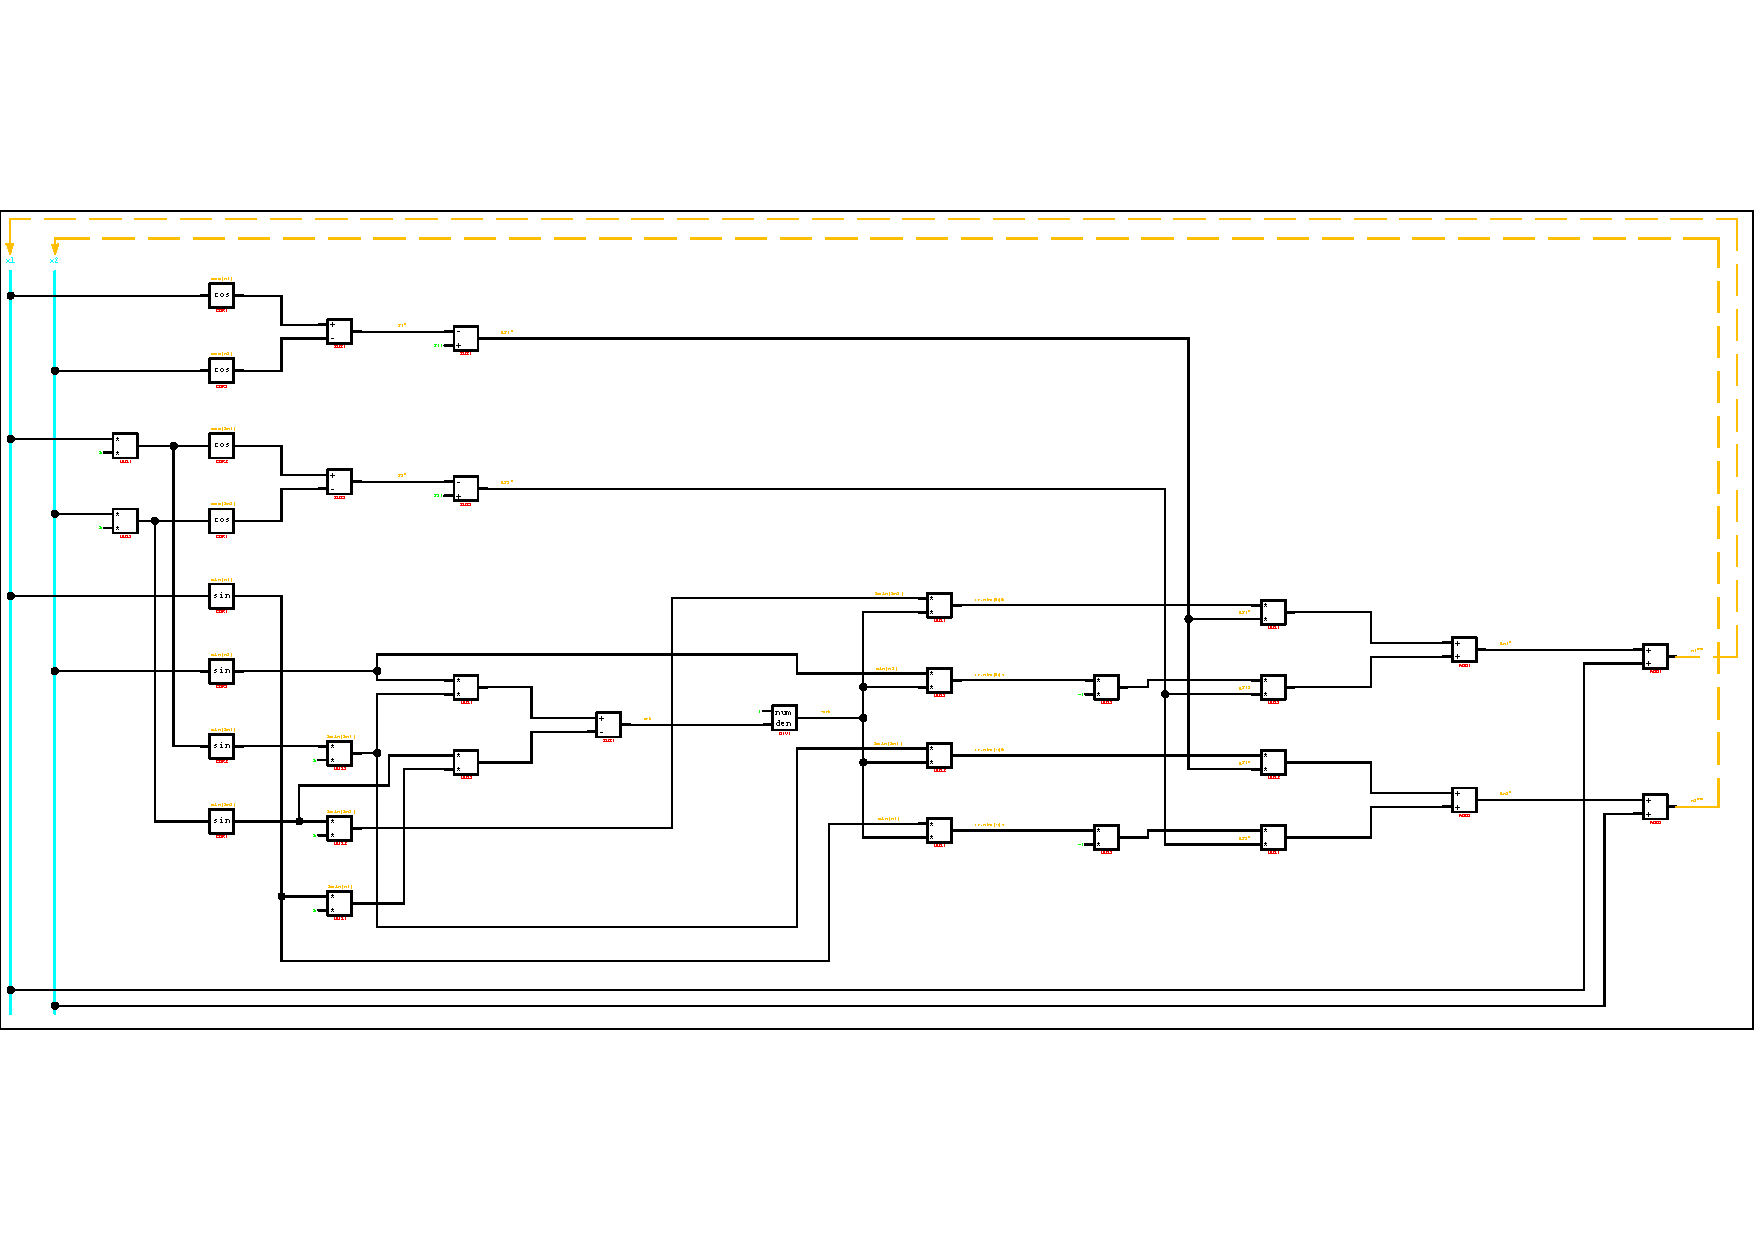
\includegraphics[width=1\textwidth]{src/pdf/she-overview.pdf}
                \caption{Block Diagram of the Selective Harmonic Elimination (\gls{abbreviation:she}) using Newton-Raphson algorithm. Design suitable for hardware implementation.}
                \label{fig:she-overview}
            \end{figure}

    \FloatBarrier
        \subsubsection{Top module design}
            The top module of this \gls{abbreviation:ip} closely resembles other developed modules in this paper. The design consists of a Control Unit which sends control signals to the Data Unit. The Data Unit, which includes registers and computational units, incorporates few external sub-modules for additional calculations, such as \gls{abbreviation:cordic} and division.\par
            Consistent with every design presented, the units utilize the \textit{Q32.15} fixed point format for the computational units and registers. The exception is the multiplier computational units, which, by the principle of multiplication, use the \textit{Q64.30} format for results. When the multiplication results are transfered to registers, the values are rounded back to the globally used format.\par
            The design is depicted in Figure \ref{fig:she-top-module}.


            \begin{figure}[htbp!]
                \centering
                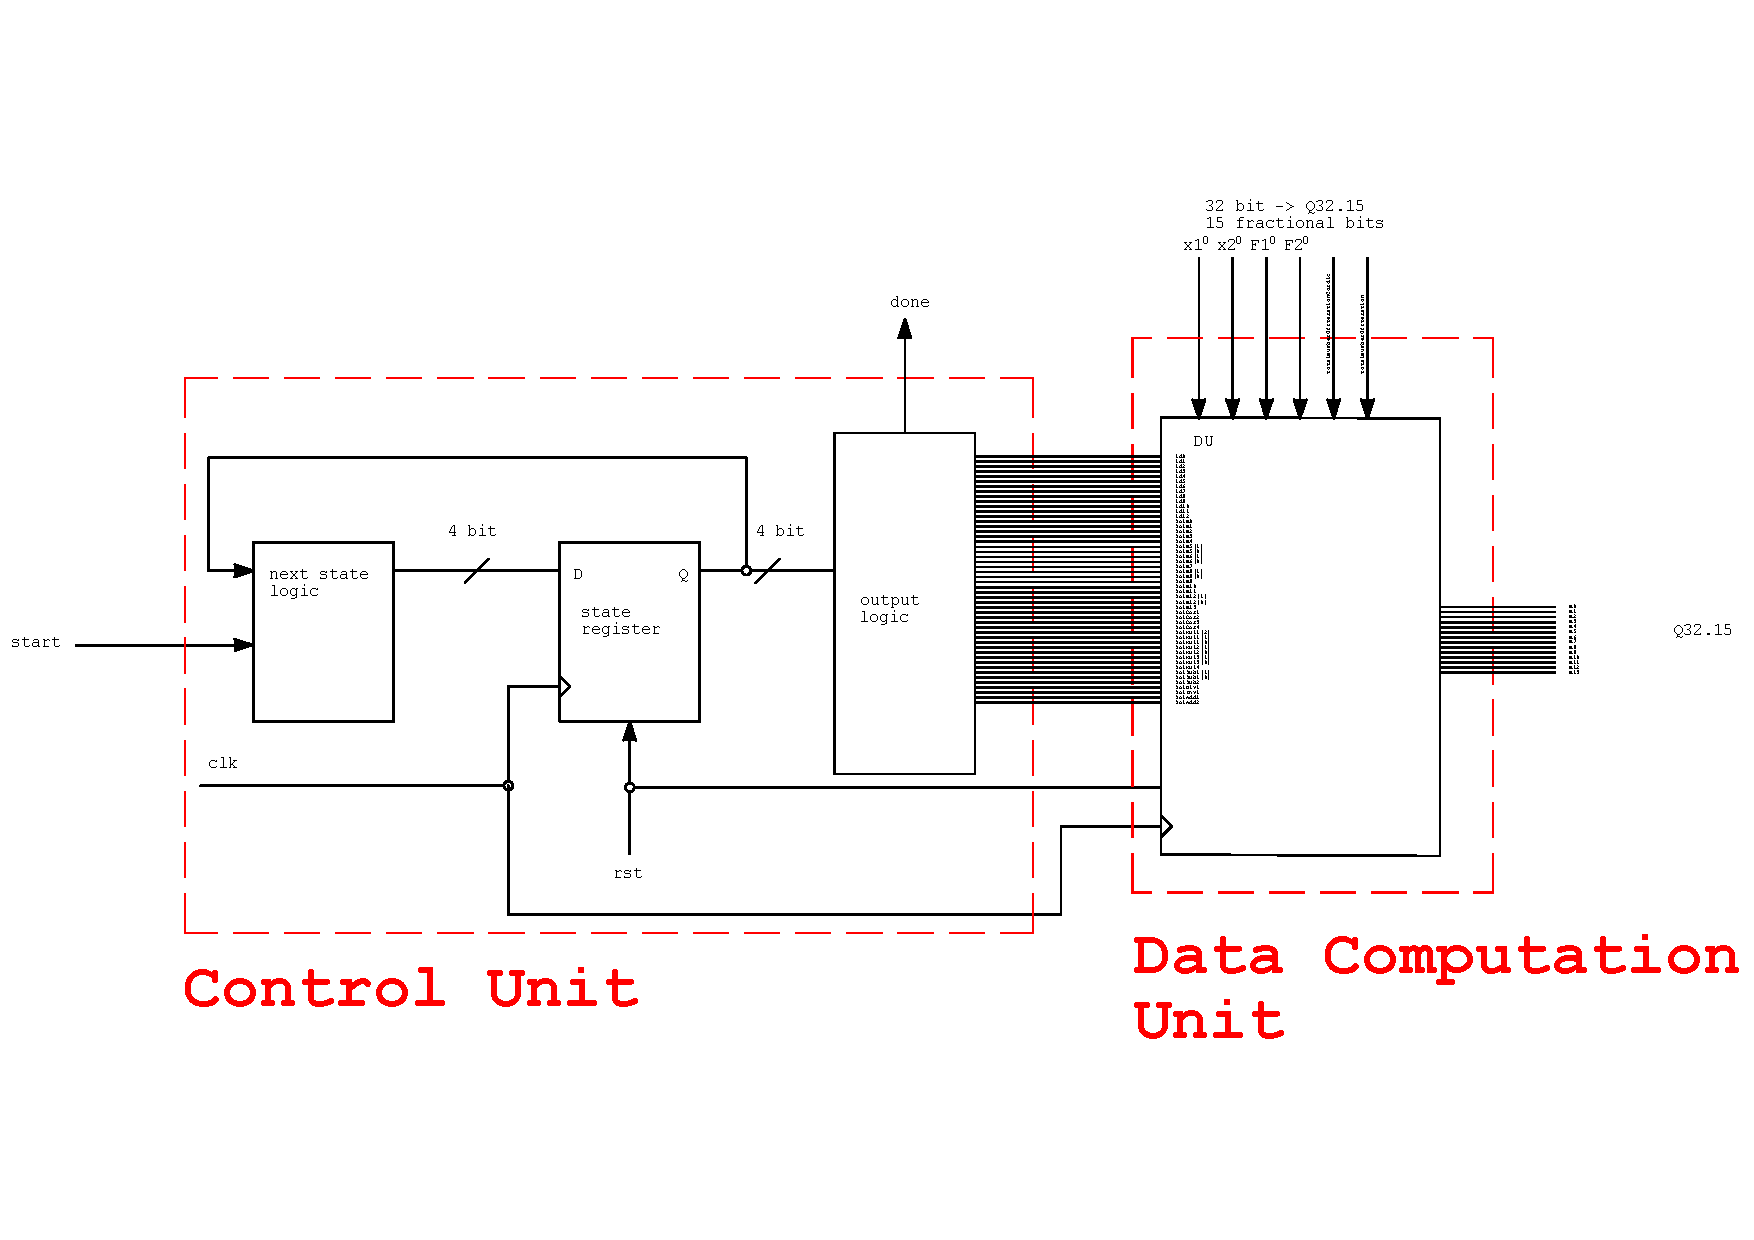
\includegraphics[width=1\textwidth]{src/pdf/she-top-module.pdf}
                           \caption{Top module design for the Selective Harmonic Elimination (\gls{abbreviation:she}).}
                \label{fig:she-top-module}
            \end{figure}

    \FloatBarrier
        \subsubsection{Allocation and Timing}\label{subsubsec:she-allocation-and-timing}
            The Allocation and Timing diagram, depicted in Figure \ref{fig:she-allocation-timing} outlines the algorithm presented in the \hyperref[subsec:she-theory]{\textit{Theory}} section. As evident from previous sections, this algorithm has been thoroughly tested before Verilog implementation.\par
            The Verilog implementation comprises a total of 13 states, labeled \textit{S0}-\textit{S12}. Through states \textit{S1}-\textit{S11}, the \gls{abbreviation:nr} algorithm iterates to calculate the final results. The state \textit{S0} is a starting state after resetting the unit, and state \textit{S12} is the ending state reached after the successful calculation of the last algorithm iteration.\par
            As previously stated, the \gls{abbreviation:she} calculation module consists of various submodules, which may use other iterative algorithms. Iterations of these submodule algorithms are not in focues of this section and are implicitly accepted as a part of the \gls{abbreviation:she} module algorithm.



            \begin{figure}[htbp!]
                \centering
                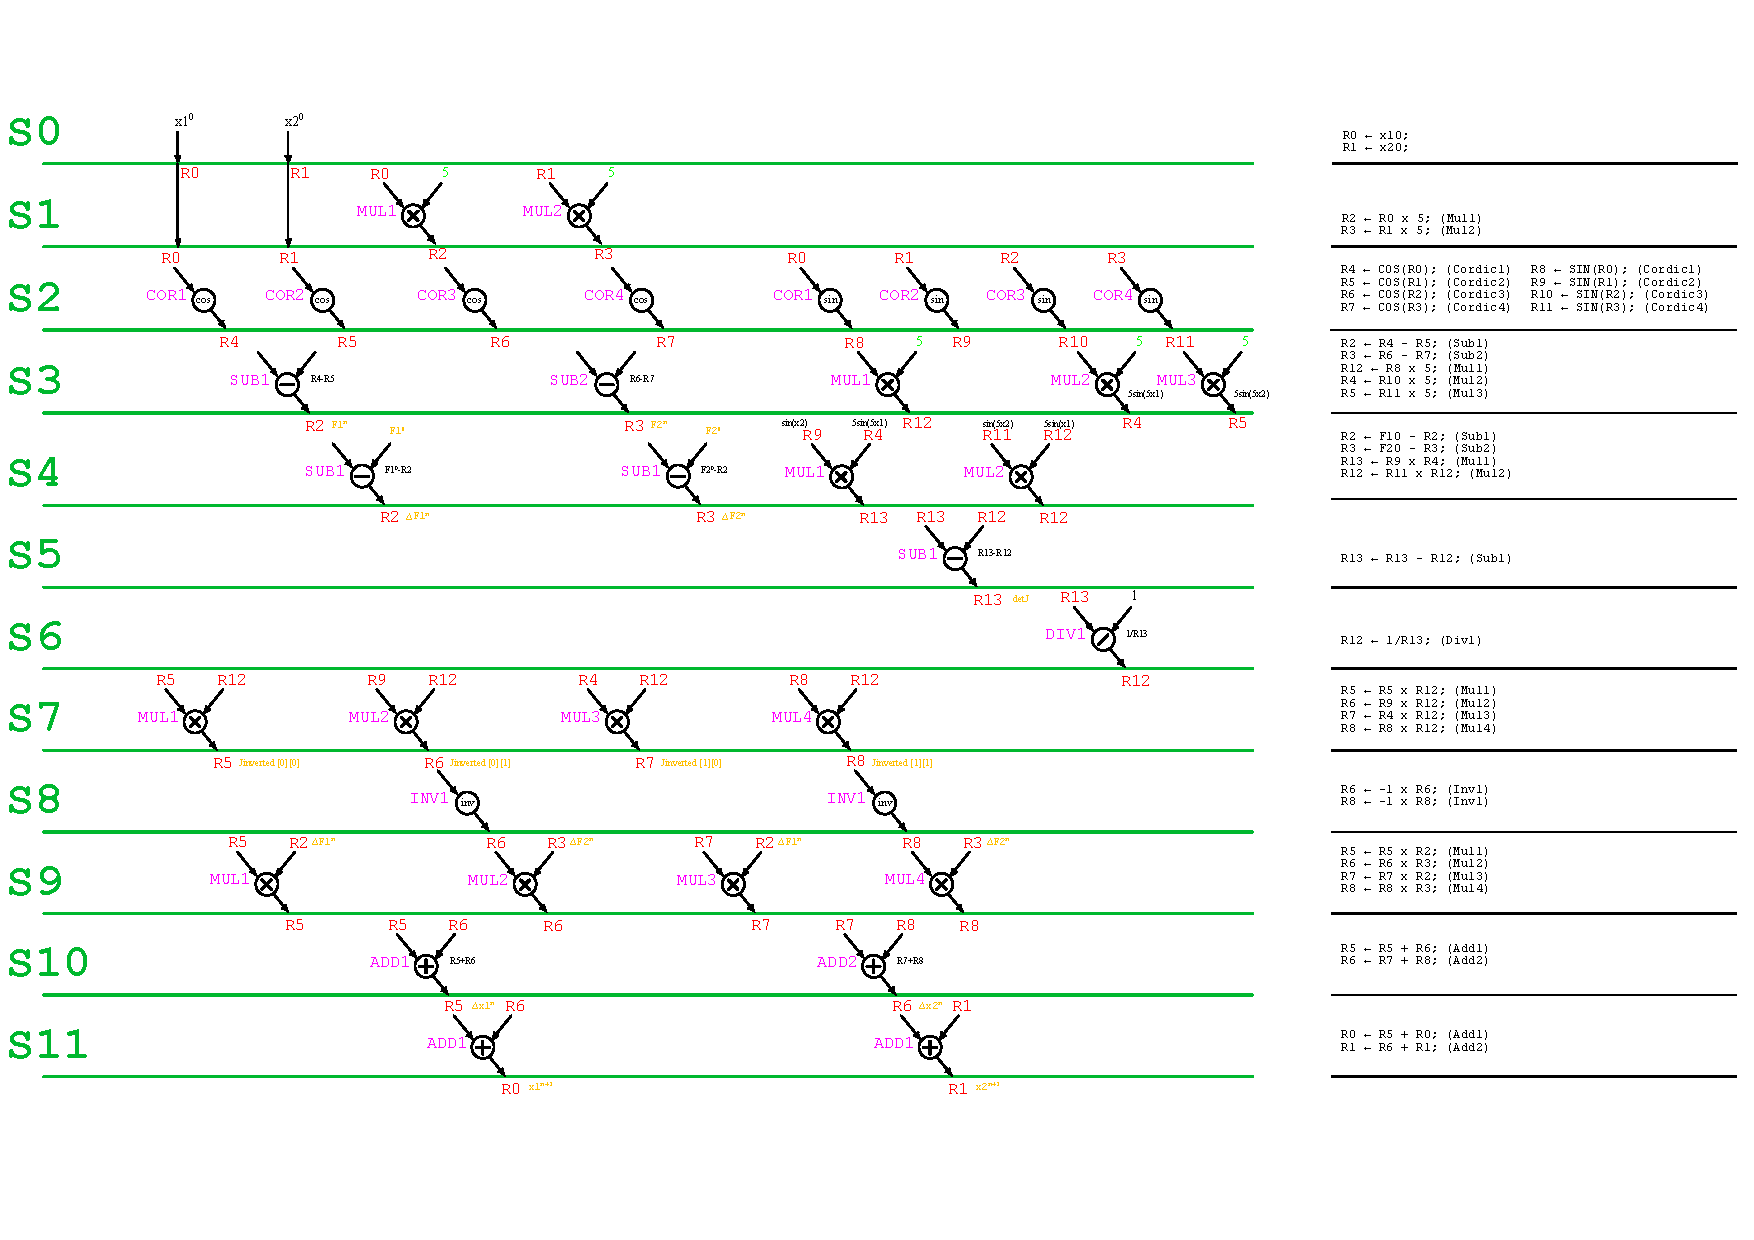
\includegraphics[width=1\textwidth]{src/pdf/she-allocation-timing.pdf}
                           \caption{Allocation and Timing diagram for the Data Path Unit part of Selective Harmonic Elimination (\gls{abbreviation:she}) module.}
                \label{fig:she-allocation-timing}
            \end{figure}

    \FloatBarrier
        \subsubsection{Data Path Unit}\label{sh:data-path-unit}
            As can be observed from the Figure \ref{fig:she-rtl} the Data Path unit for solving the transcendetal equations is more complex than previously presented units. Obviously the design could be further simplified, i.e., reduce the number of registers and calculation units. This simplification would result in a trade of speed for less complexity. The less complex the design, the less \gls{abbreviation:fpga} resources, i.e., \gls{abbreviation:lut}s, is needed for the realization of the design. This paper mainly focuses on speed and clarity, so the design consists of thirteen data registers, four \gls{abbreviation:cordic} units, four multiplication units, two adders, two subtractors, one division unit and one invertor unit, which is implemeted directly in the registers logic.
            \begin{figure}[htbp!]
                \centering
                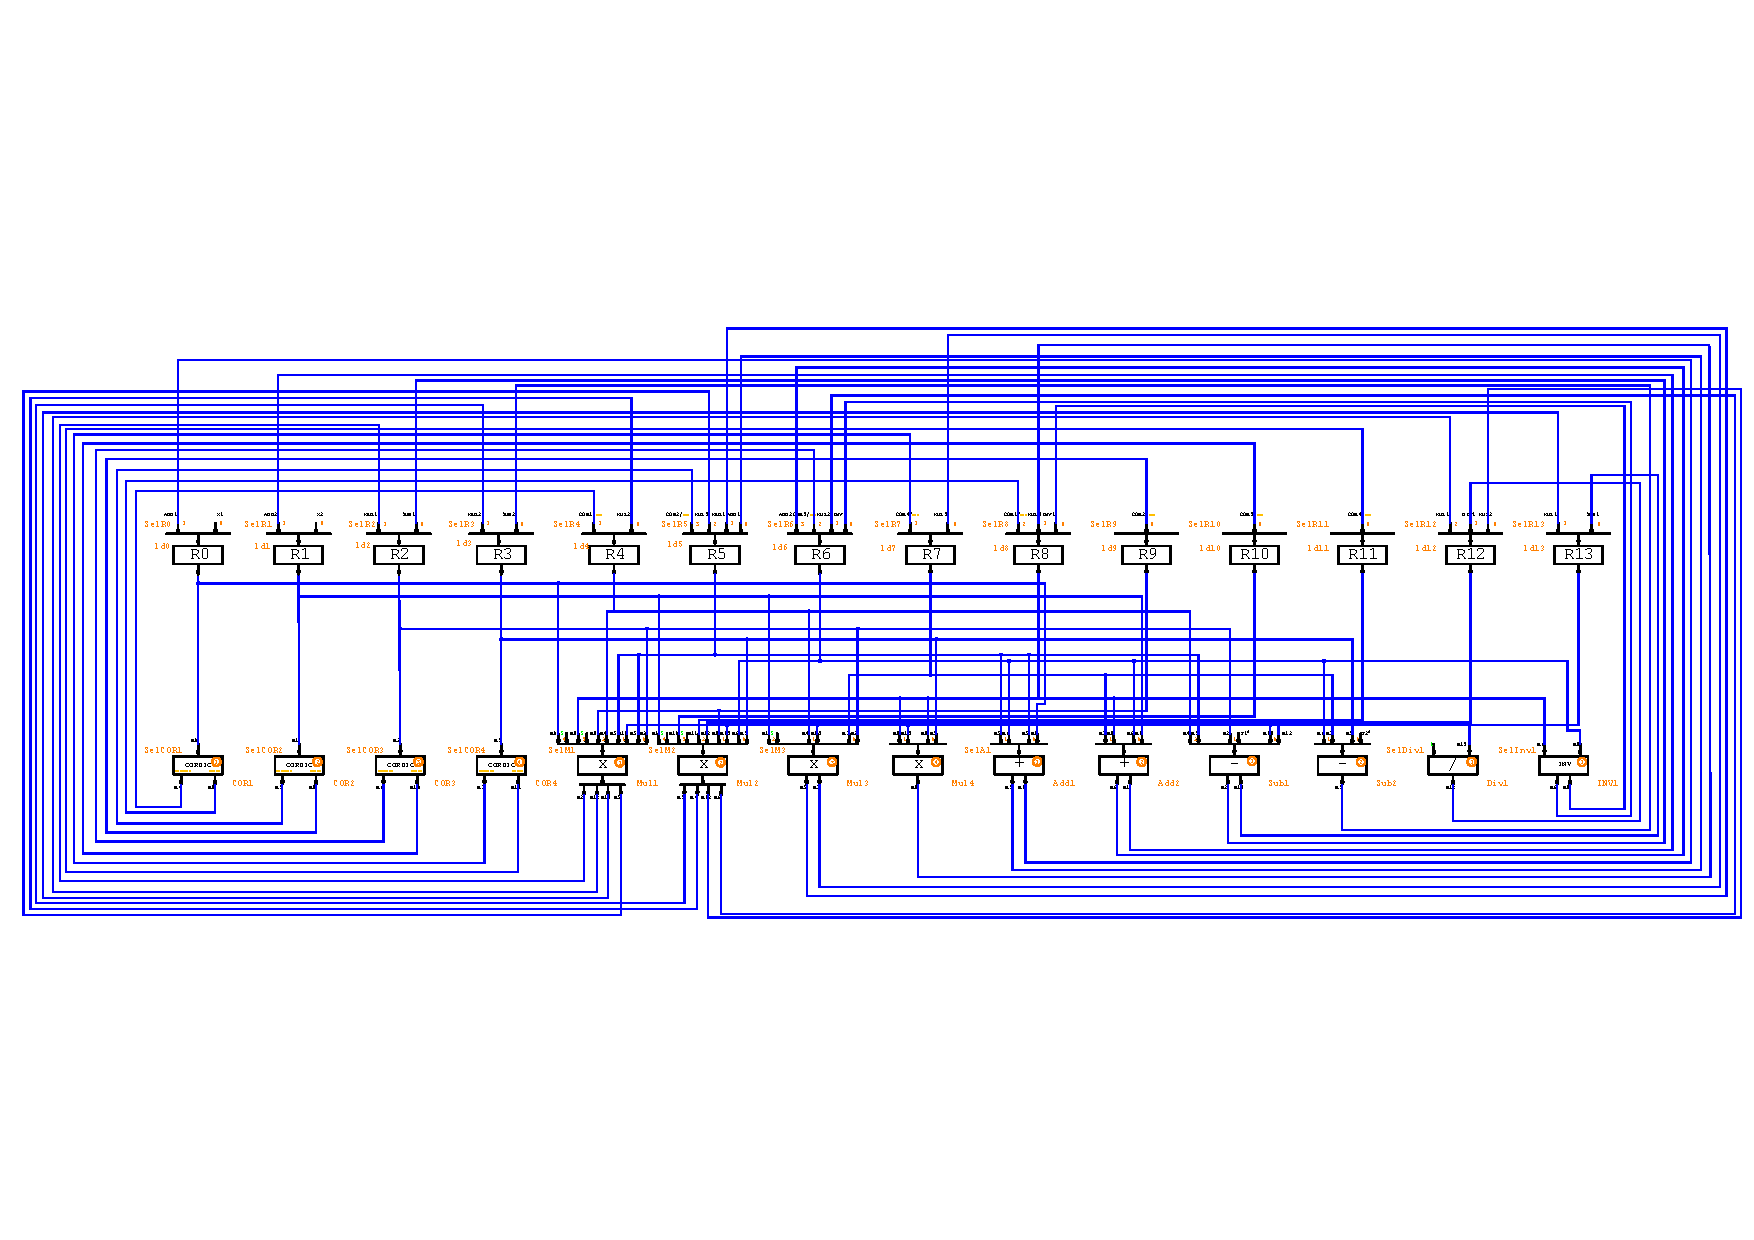
\includegraphics[width=1\textwidth]{src/pdf/she-rtl.pdf}
                \caption{Register transfer level (\gls{abbreviation:rtl}) scheme of the Selective Harmonic Elimination Data Path Unit.}
                \label{fig:she-rtl}
            \end{figure}
    
    \FloatBarrier
        \subsubsection{Control Unit}\label{subsubsec:sh-elimination-control-unit}
            Control unit signal specification can be observed in the Table \ref{tab:control-signal-she-unit}. If the unit design was less complex, i.e., with smaller amount of registers, the control signal length would be smaller, but the number of states would be higher.

        \subfile{src/tex/sh-elimination-control-unit-table.tex}
    \FloatBarrier

    \subsubsection{Inverter output voltage analysis for Verilog implementation}
        The simulated \gls{abbreviation:vsi} output phase voltage, when the \gls{abbreviation:she} algorithm is employed for the modulation index $m = 1$ in Verilog, is depicted in the Figure \ref{fig:VerilogPlotWaveform}. The harmonic analysis for the presented waveform can be observed in the Figure \ref{fig:VerilogPlotHarmonics}. As mentioned in previous sections, please note that in the 3-phase symmetrical system, the triplen harmonics would be eliminated as well. It is evident that the unwanted 5th harmonics has been successfully eliminated. The calculated angles after ten iterations of the \gls{abbreviation:nr} algorithm are $\alpha_1 = 0.06341$ rad and $\alpha_2 = 1.320098$ rad.

            \begin{figure}[htbp!]
                \centering
                \begin{subfigure}[t]{0.45\textwidth}
                    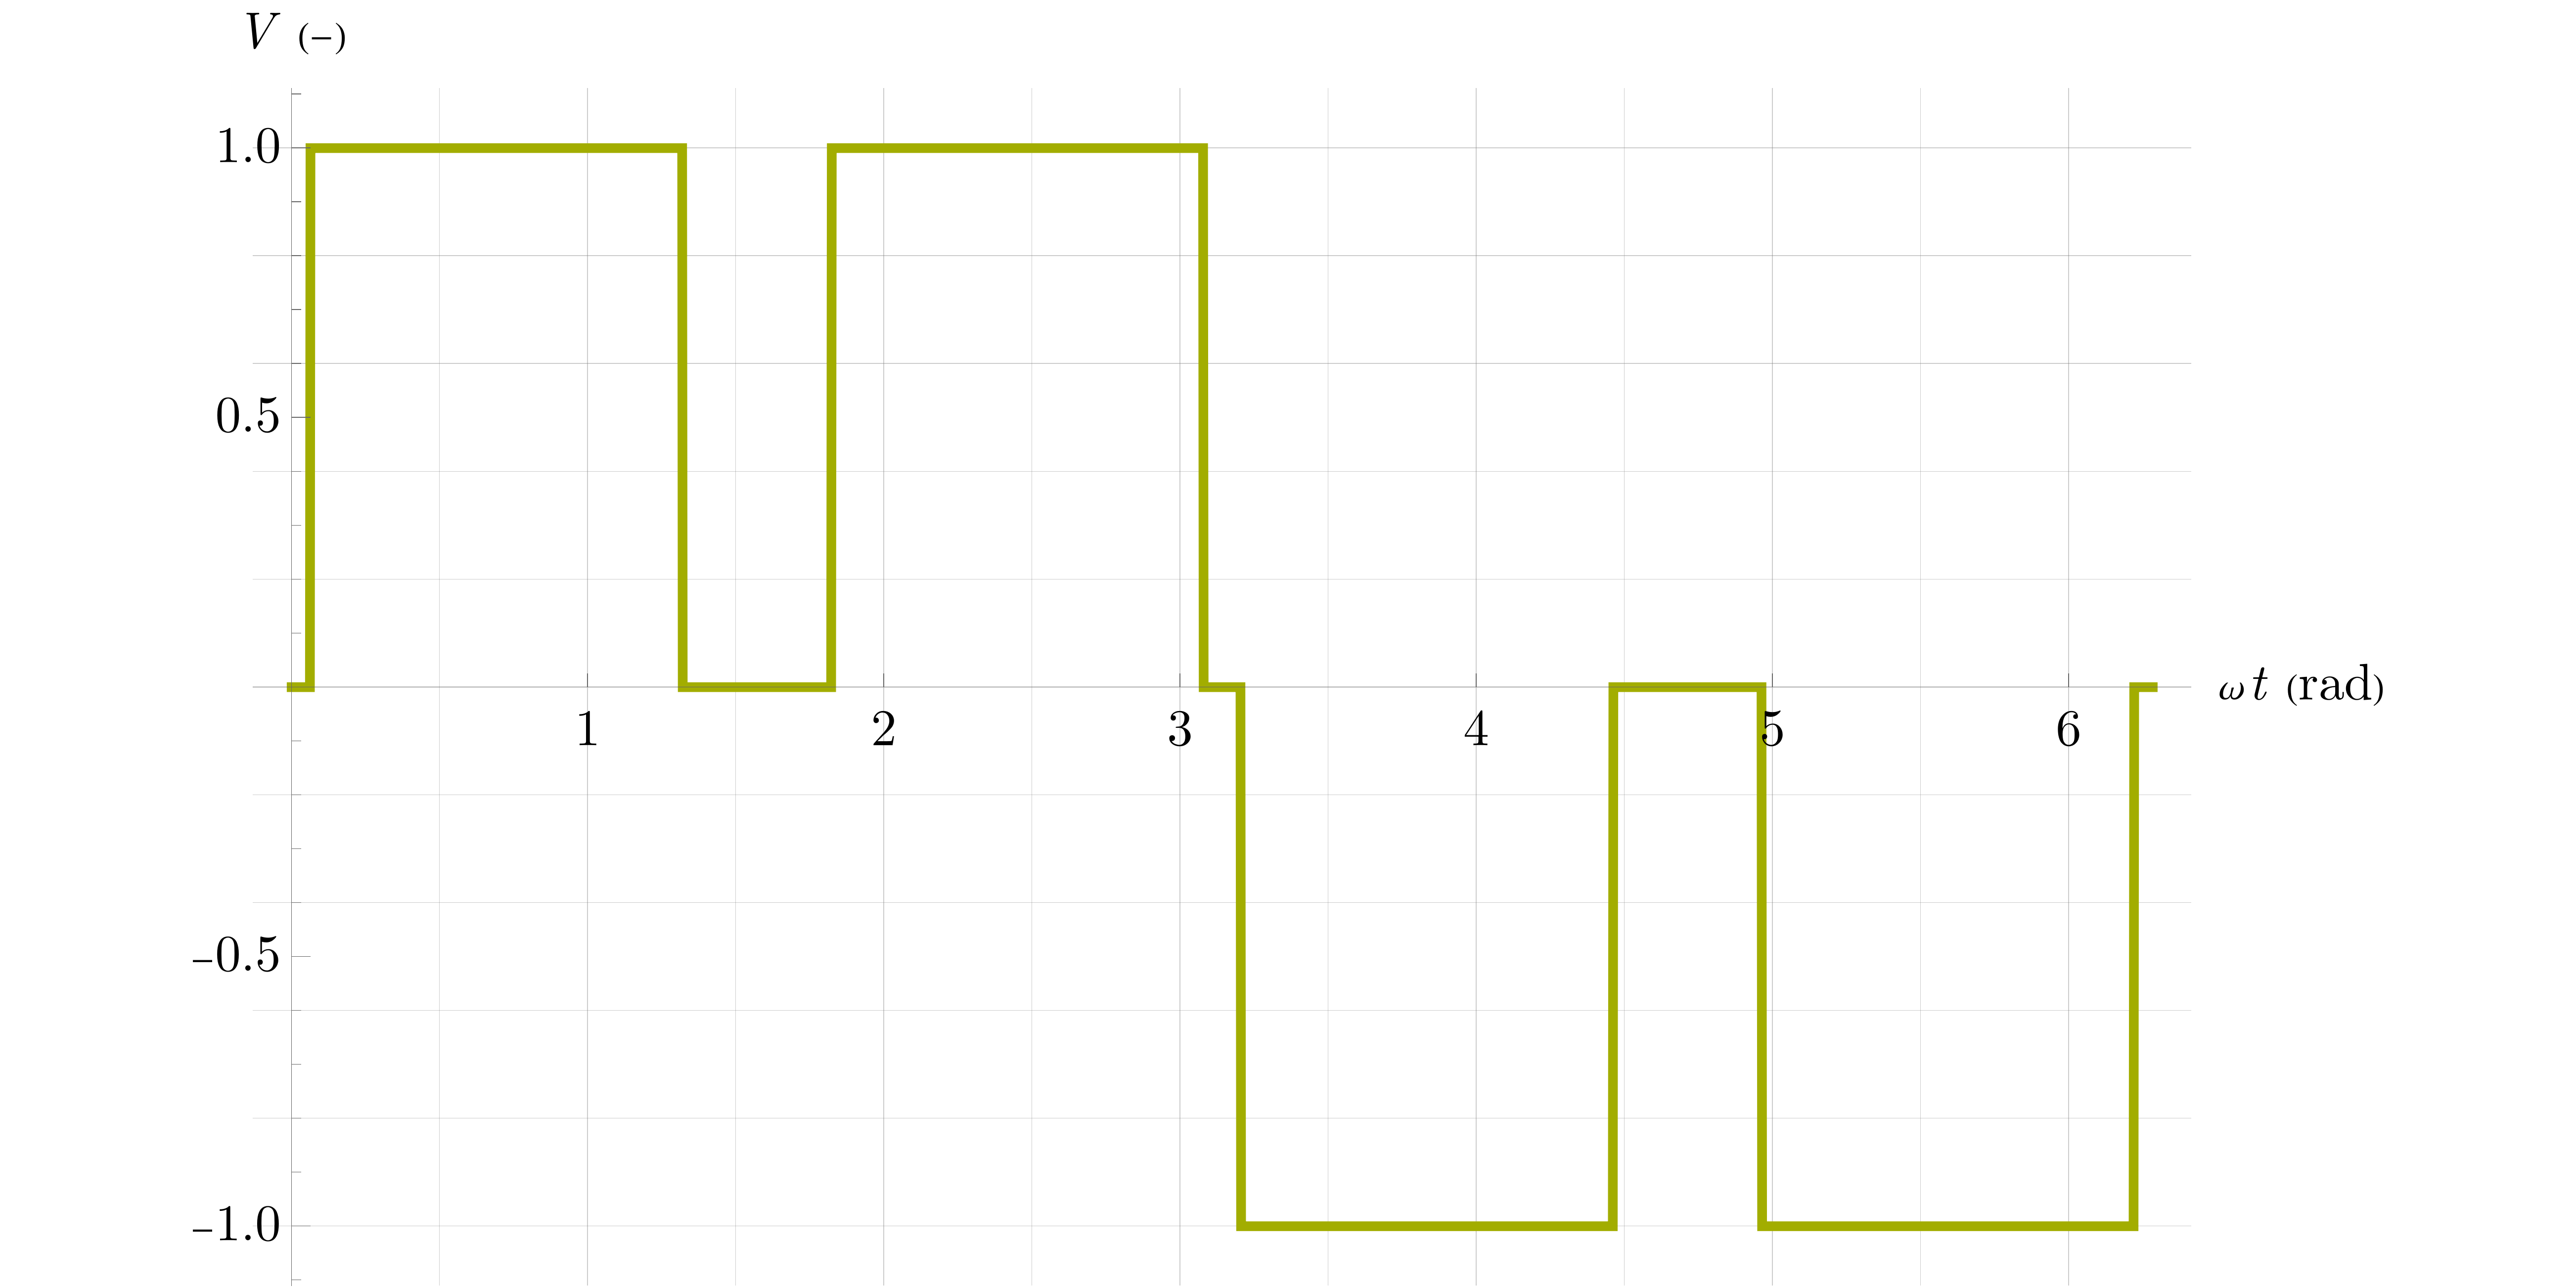
\includegraphics[width=1\textwidth]{src/png/VerilogPlotWaveform.png}
                    \caption{Waveform output of a two level Voltage Source Inverter when the Selective Harmonic Elimination method is applied with Verilog calculated angles. The Voltage value is normalized to a \gls{abbreviation:dc} link voltage.}
                    \label{fig:VerilogPlotWaveform}
                \end{subfigure}
                \hspace{0.05\textwidth}
                \begin{subfigure}[t]{0.45\textwidth}
                    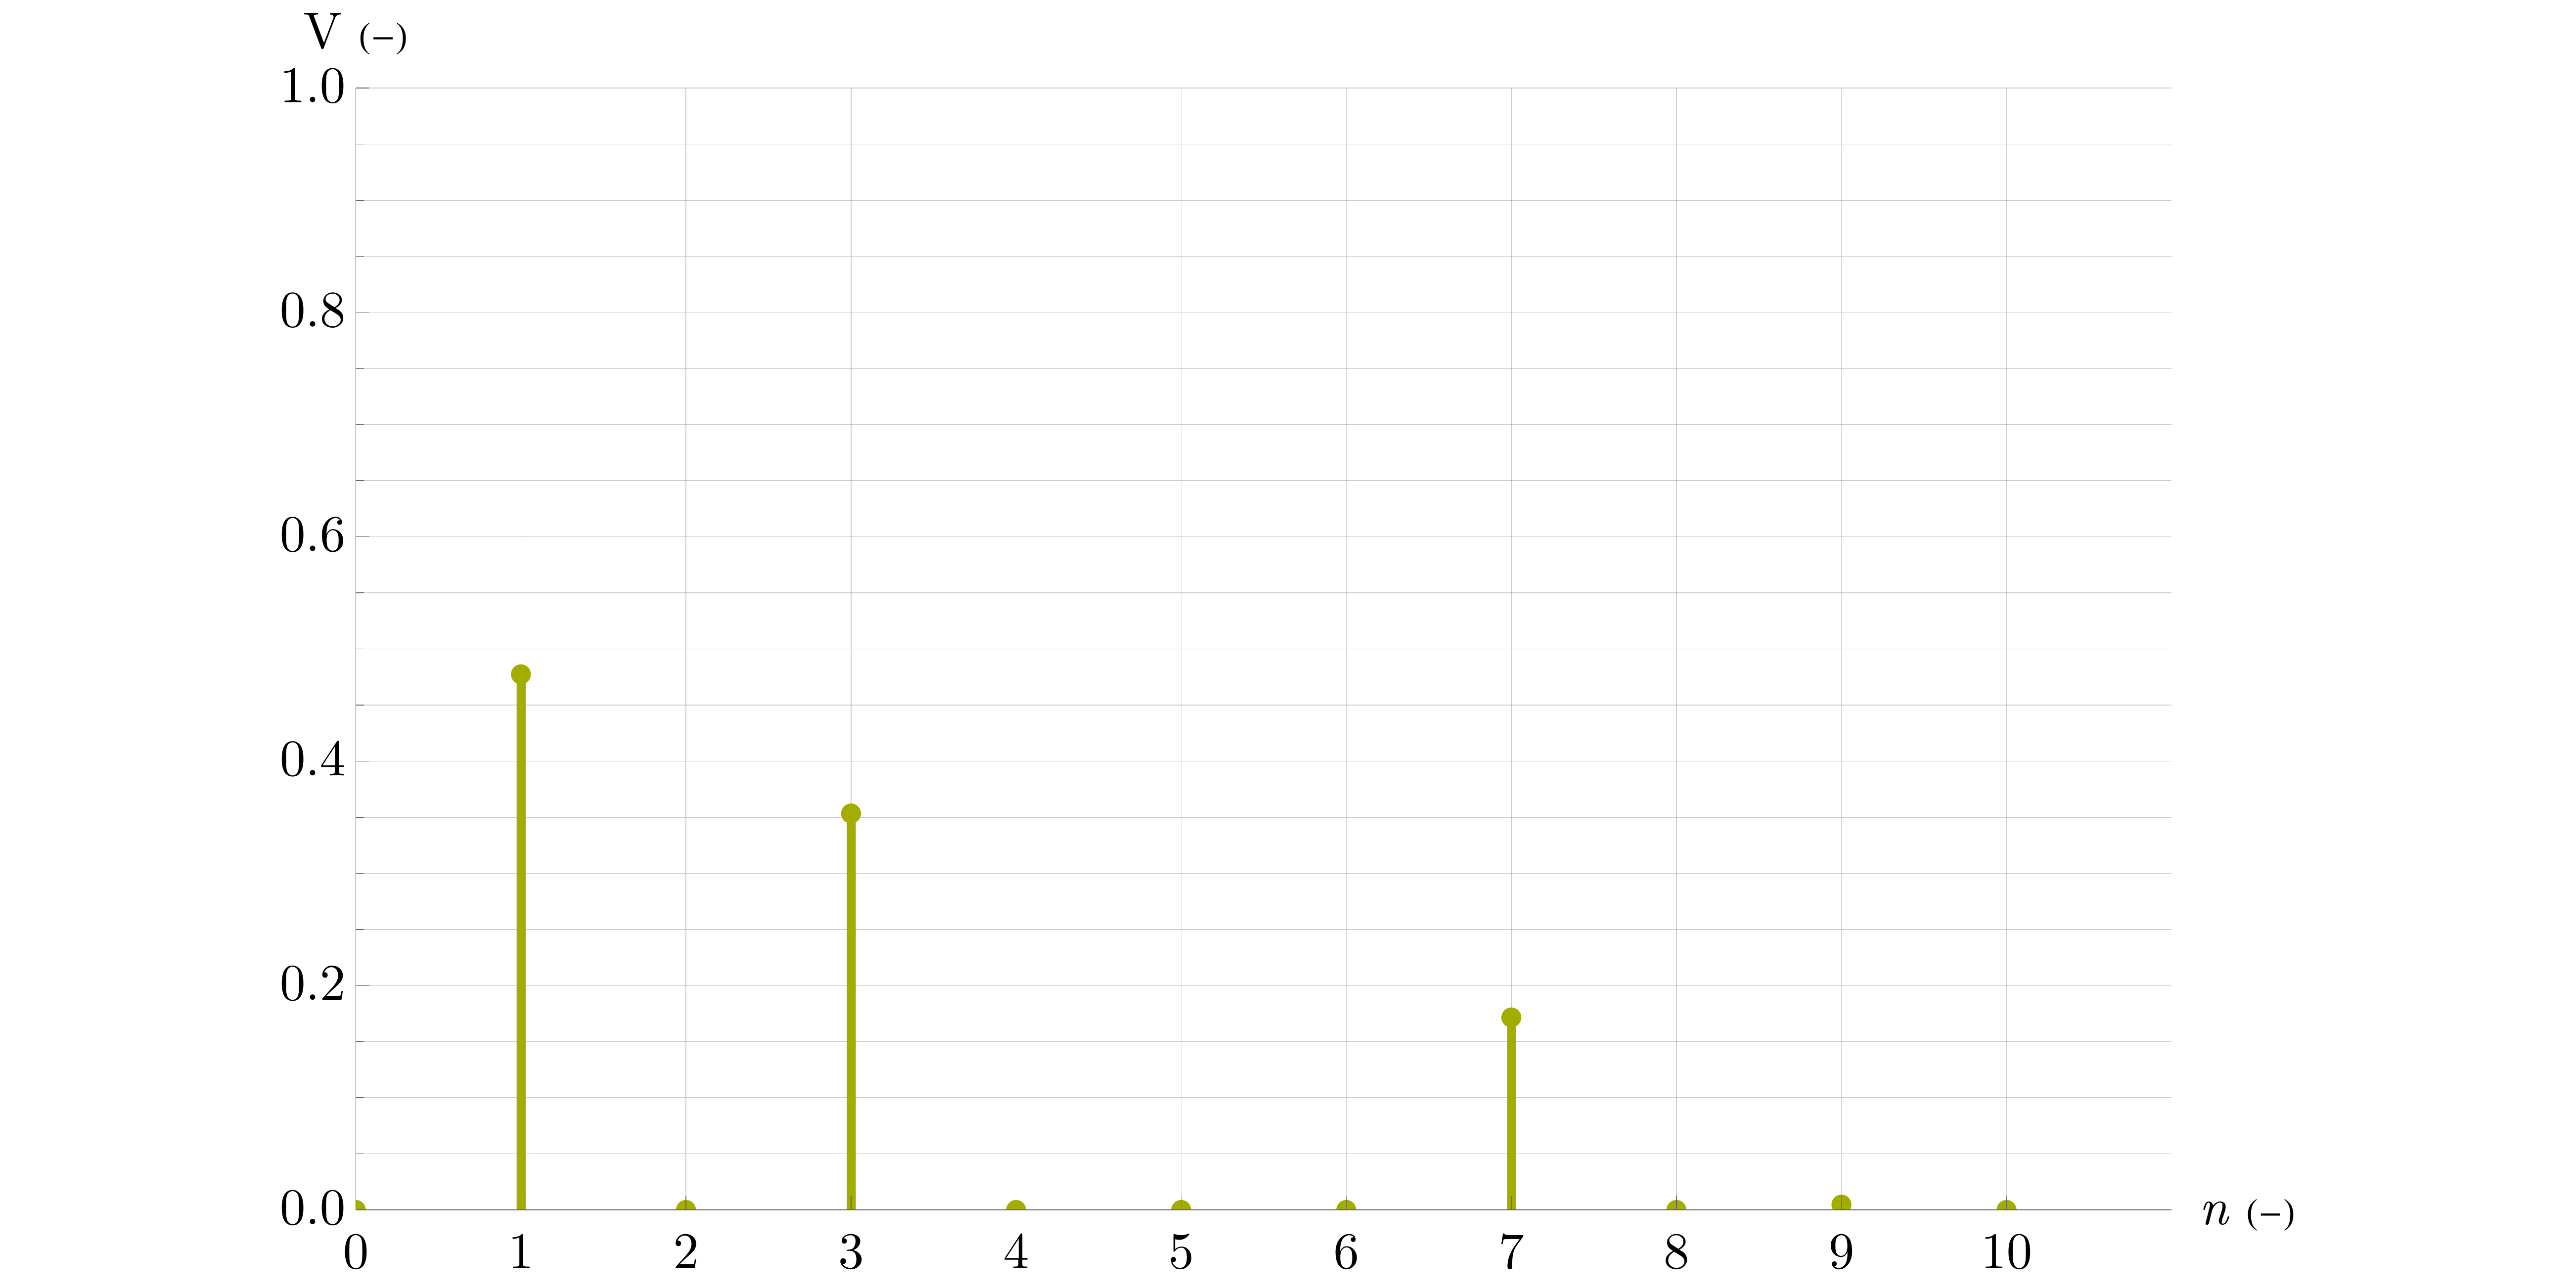
\includegraphics[width=1\textwidth]{src/png/VerilogPlotHarmonics.png}
                    \caption{Waveform harmonics analysis of a output voltage of a two level Voltage Source Inverter utilising switching angles for the Selective Harmonic Elimination calculated in Verilog unit. The Voltage value is normalized to a DC link voltage.}
                    \label{fig:VerilogPlotHarmonics}
                \end{subfigure}
                \caption{}
            \end{figure}

            \begin{figure}[htbp!]
                \centering
                \begin{subfigure}[t]{0.45\textwidth}
                    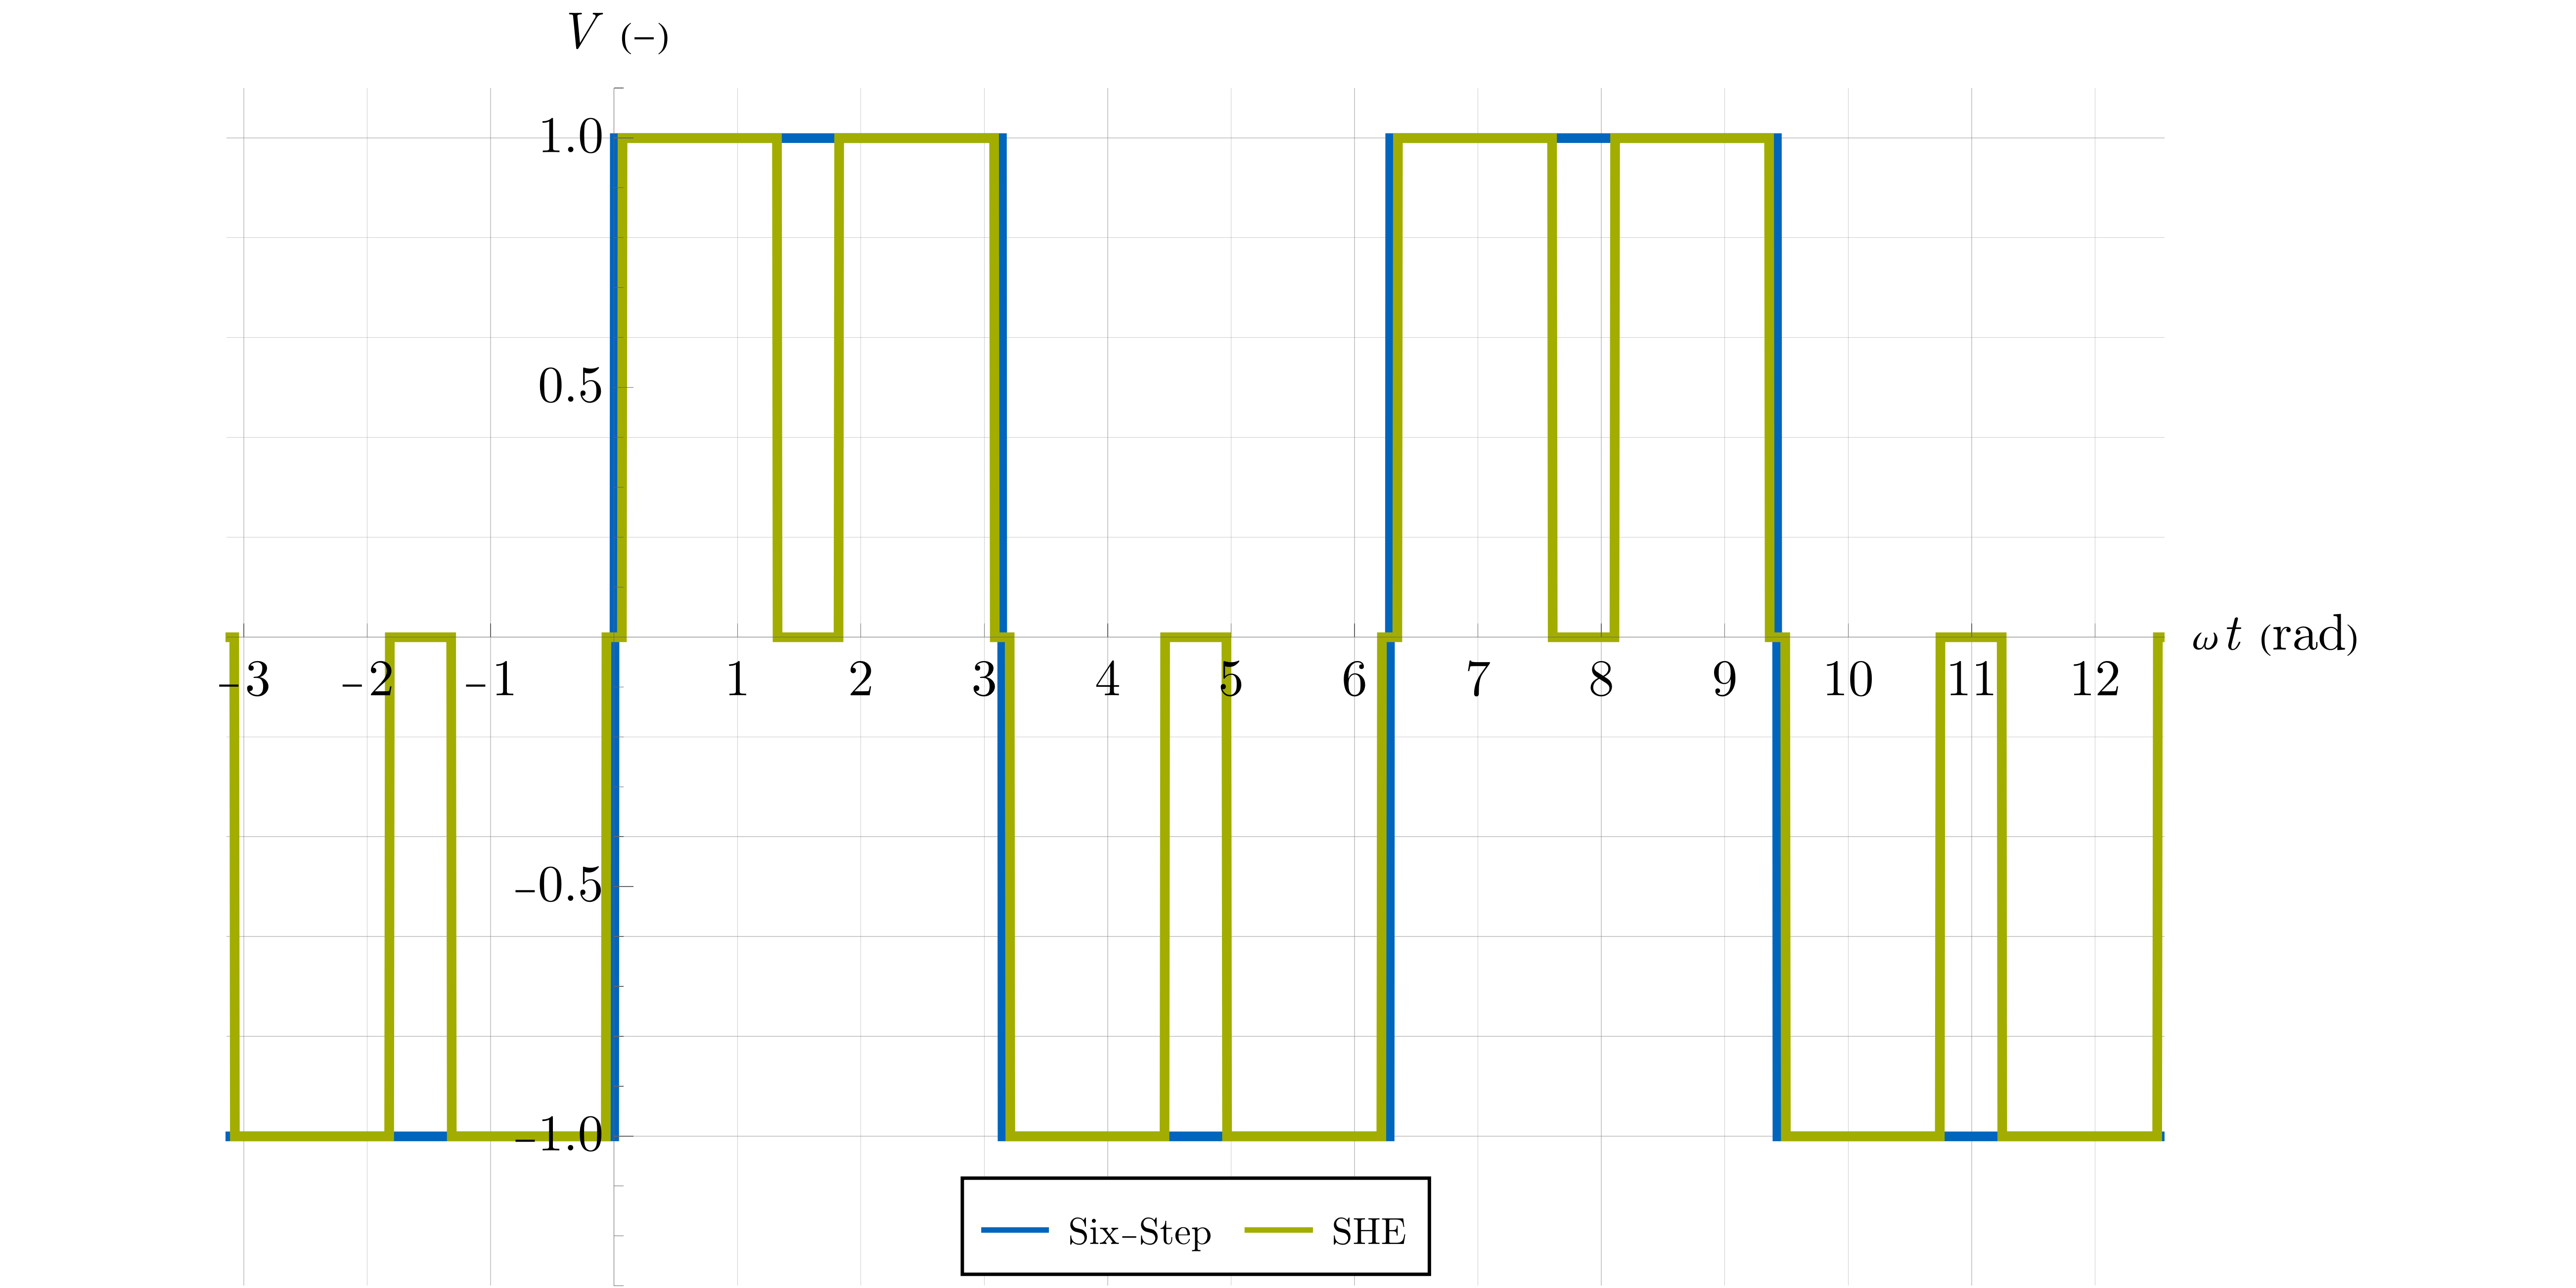
\includegraphics[width=1\textwidth]{src/png/ComparisonPlotSixStepVerilogSheWaveform.png}
                    \caption{Comparison of a Waveform output of a two level Voltage Source Inverter when the Selective Harmonic Elimination method is or is not applied with Verilog calculated angles. The Voltage value is normalized to a \gls{abbreviation:dc} link voltage.}
                    \label{fig:ComparataionPlotSixStepVerilogSheWaveform}
                \end{subfigure}
                \hspace{0.05\textwidth}
                \begin{subfigure}[t]{0.45\textwidth}
                    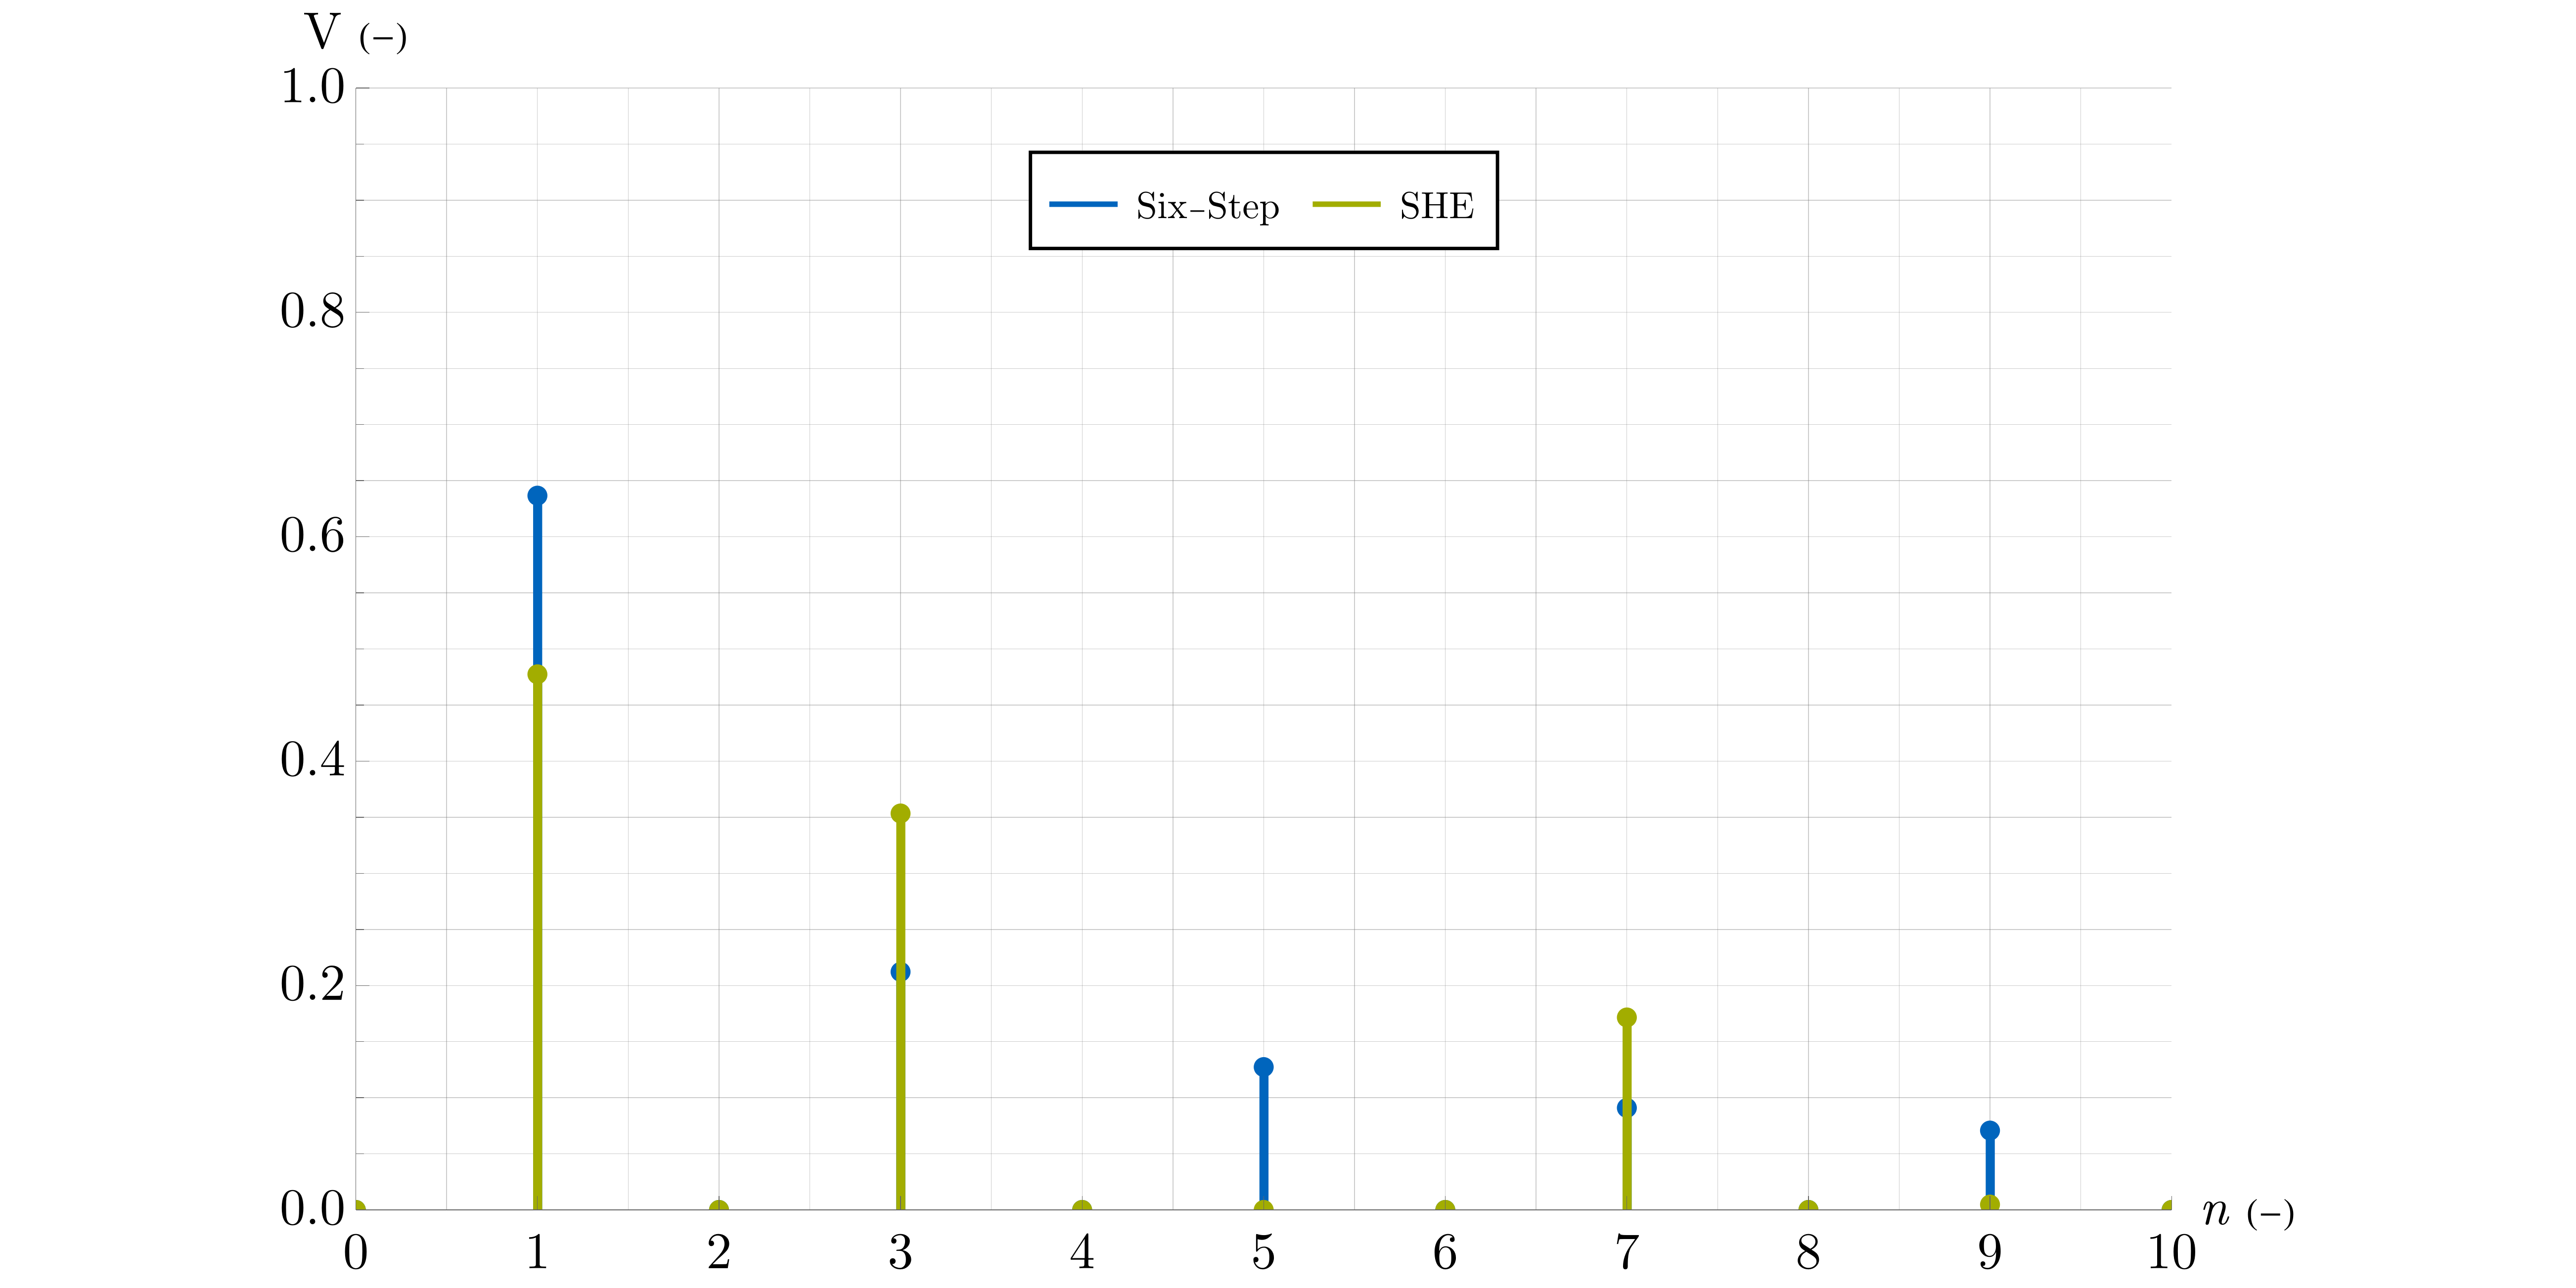
\includegraphics[width=1\textwidth]{src/png/ComparisonPlotSixStepVerilogSheHarmonics.png}
                    \caption{Comparison of a Waveform harmonics analysis of a output voltage of a two level Voltage Source Inverter with and without the Selective Harmonic Elimination. The Voltage value is normalized to a DC link voltage.}
                    \label{fig:ComparataionPlotSixStepVerilogSheHarmonics}
                \end{subfigure}
                \caption{}
            \end{figure}
            \FloatBarrier

    \subsection{Simulation results}
        The end of simulation with result of \gls{abbreviation:she} alogrithm after the 10th \gls{abbreviation:nr} algorithm can be seen in Figure \ref{fig:she-sim-end}. The whole simulation run is depicted in the Figure \ref{fig:she-sim-all}.\par
        The clock signal frequency in simulation was set to 25 MHz to emulate low cost \gls{abbreviation:fpga} capabilities.
            \begin{figure}[htbp!]
                \centering
                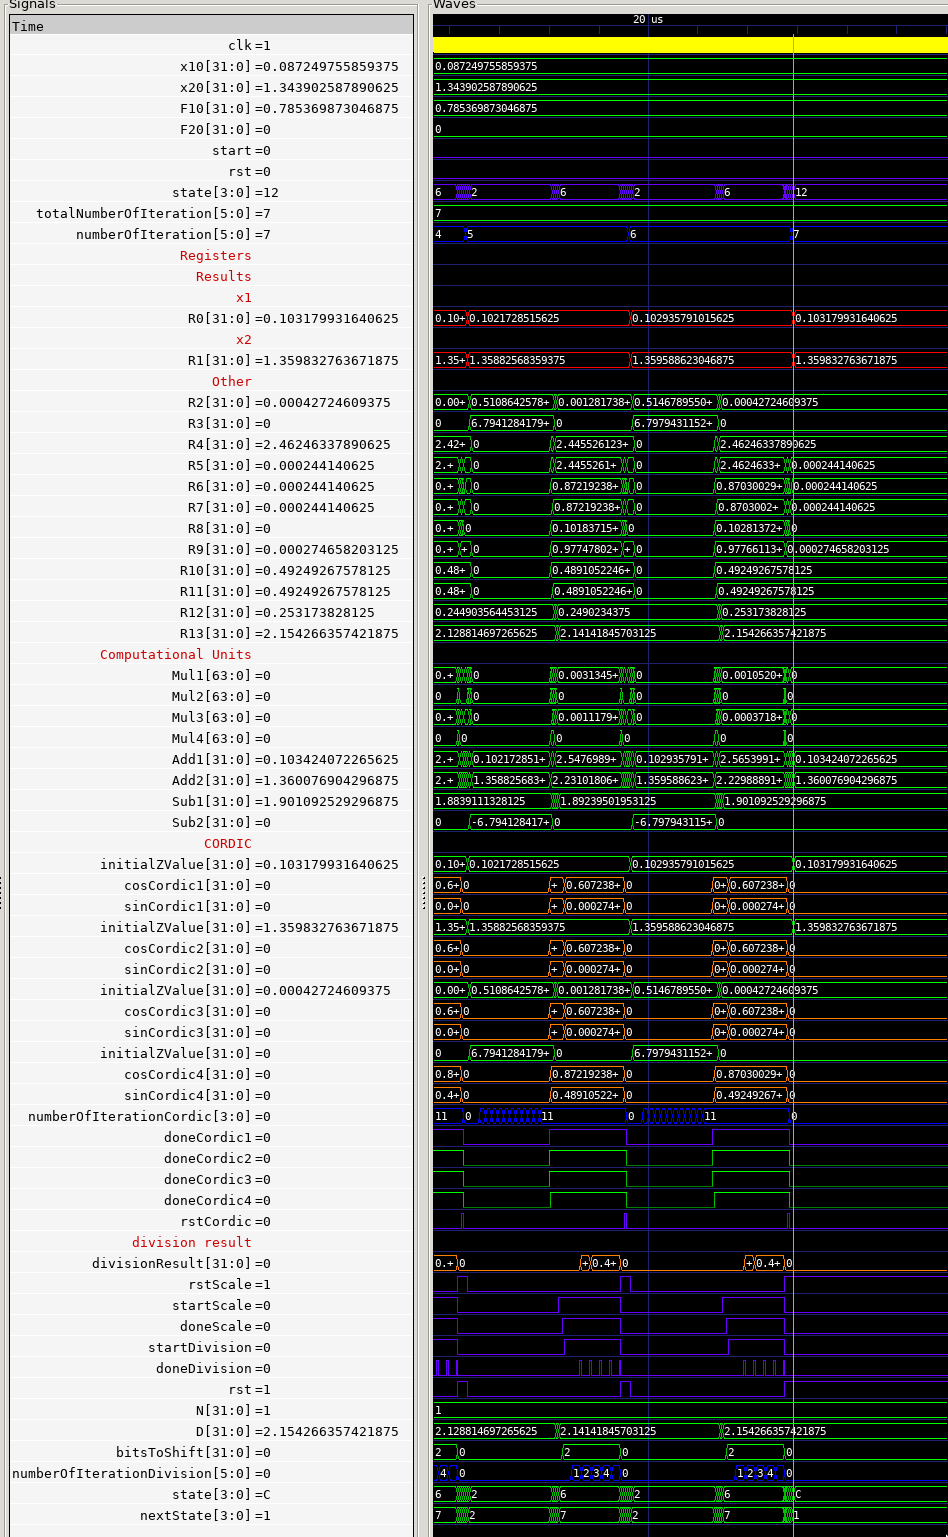
\includegraphics[width=1\textwidth]{src/png/she-sim-end.png}
                \caption{The ending part of a Verilog simulation of Selective Harmonic Elimination (\gls{abbreviation:she}) algorithm. The result are in registers R0 and R1.}
                \label{fig:she-sim-end}
            \end{figure}

            \begin{figure}[htbp!]
                \centering
                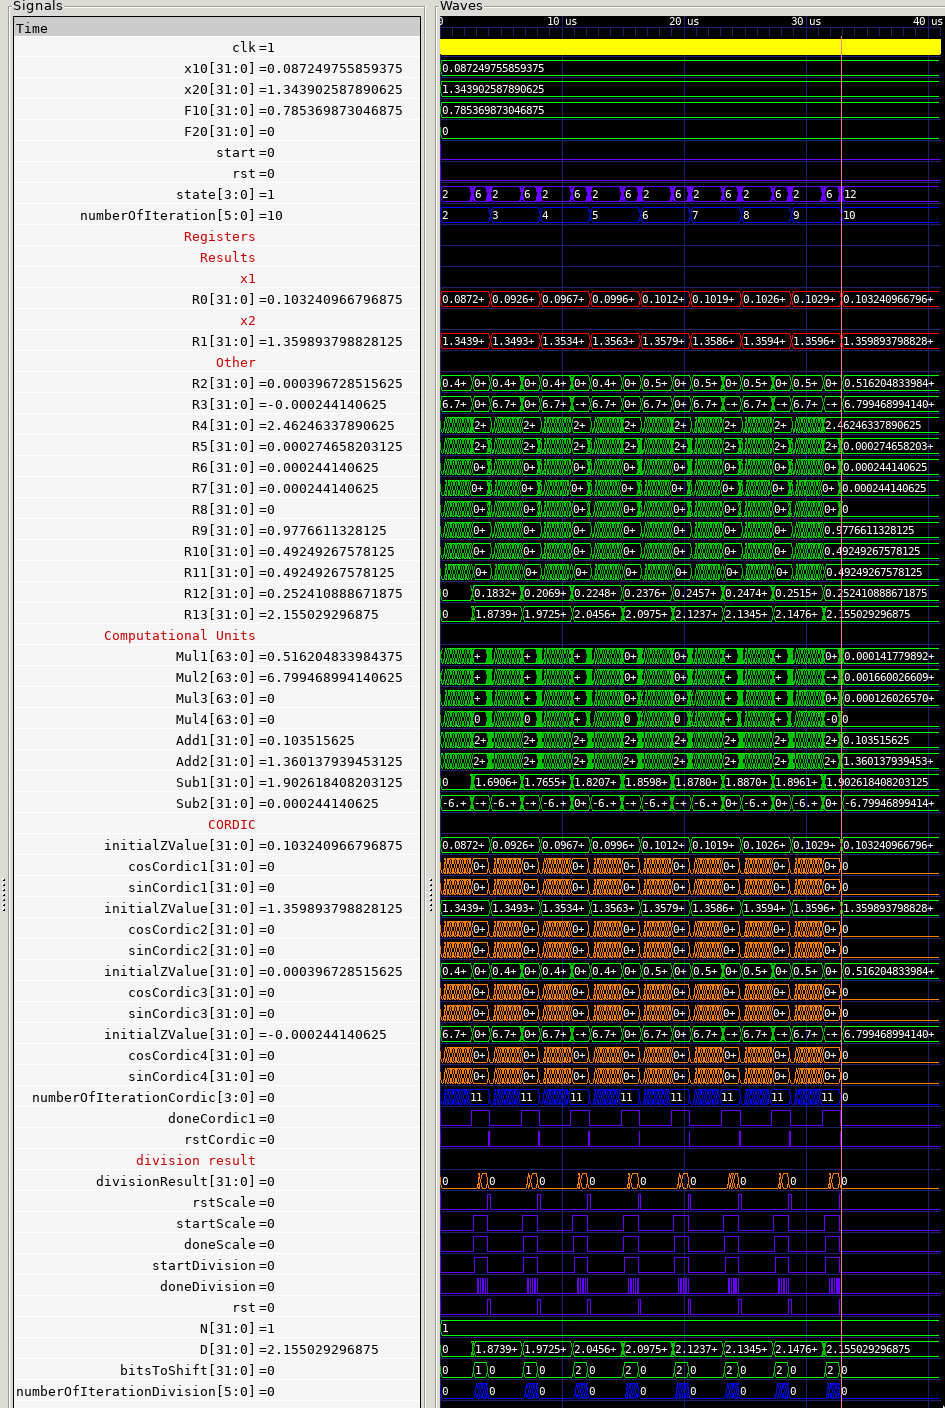
\includegraphics[width=1\textwidth]{src/png/she-sim-all.png}
                \caption{The whole Verilog simulation of Selective Harmonic Elimination (\gls{abbreviation:she}) algorithm. The result are in registers R0 and R1.}
                \label{fig:she-sim-all}
            \end{figure}
%závěr
\newpage
\addcontentsline{toc}{section}{\numberline{}Conclusion} 
\section*{Conclusion}
This paper introduces \gls{abbreviation:fpga} module designed for solving the \gls{abbreviation:she} algorithm in near real-time. The module comprises two additional submodules, both discussed in this paper. These submodules include units for calculating the division of two arbitrary values and a \gls{abbreviation:cordic} unit suitable for calculating $sine$ and $cosine$ functions.\par
The primary objective of this paper was to design speed-optimized modules capable of near real-time calculations. The outcomes of this paper could serve as a starting point for future research in designing modules for controlling electric drives or creating Hardware-in-Loop Systems.

\flushbottom %vyčištění stránky

%konec závěru

\newpage
\setmonofont{Times New Roman}
\printbibliography[title={{References}}]	
\nocite{*}
\setmonofont{CourierPrime-Regular}
\addcontentsline{toc}{section}{\numberline{}References} %Added citations to TOC%
	\appendix
	\titleformat{\section}{\color{ctublue}\fontspec{Times New Roman}\fontsize{15}{15}\bfseries}{Appendix \thesection:}{2.1em}{}
	\begin{appendices}
	\section{List of and Abbreviations}
		\printglossary[type=abbreviationslist, style = myStyleAbbreviations]
		\fbar
		%\printglossary[type=symbolslist, style =  myStyleSymbols]
	\end{appendices}
\end{document}
